\documentclass[a4paper,10pt]{book}
\usepackage{graphicx} %\usepackage[utf8]{inputenc}

% headers and footers
\usepackage{fancyhdr}
\setlength{\headheight}{15.2pt}


\pagestyle{fancy}
\renewcommand{\chaptermark}[1]{ \markboth{#1}{} }

\renewcommand{\sectionmark}[1]{ \markright{#1} }
%\renewcommand*{\chaptermark}[1]{ \markboth{\chaptername\ \thechapter: ##1}{} }%
\fancyhf{}
\fancyhead[RE,LO]{} %\thepage }
\fancyhead[LE]{\textit{\thepage \phantom{mmmm}  \thechapter.\ \nouppercase{\leftmark}}}
\fancyhead[RO]{\textit{\S  \thesection \phantom{m} \nouppercase{\rightmark} \phantom{mmmm} \thepage } }



\fancypagestyle{plain}{%  the preset of fancyhdr 
    \fancyhf{} % clear all header and footer fields
    \fancyfoot[C]{ \thepage} %\textbf{\thepage}} % except the center
    \renewcommand{\headrulewidth}{0pt}
    \renewcommand{\footrulewidth}{0pt}}


% \fancypagestyle{myheadings}{%
%  \fancyhf{}
%  \renewcommand{\headrulewidth}{0.05pt}
%  \renewcommand{\footrulewidth}{0.02pt}
%  \addtolength{\headheight}{0.5pt}
%  \fancyhead[LE,RO]{\thechapter}
%  \fancyhead[RE,LO]{Section \thesection}
%  \fancyfoot[CE,CO]{\leftmark}
%  \fancyfoot[RO,LE]{\thepage}
%}


 
%\pagestyle{myheadings}
  \pagestyle{fancy}



  
%center all figures:
\makeatletter
\g@addto@macro\@floatboxreset\centering
\makeatother

\usepackage{bbold}

\usepackage{imakeidx}

\makeindex

\usepackage[square,sort,comma,numbers]{natbib}

\usepackage{amsmath}
\usepackage{bm}

\usepackage[sc]{mathpazo}
\linespread{1.05} % Palladio needs more leading (space between lines)
\usepackage[T1]{fontenc}

\usepackage{siunitx}

\usepackage{showlabels}

% \usepackage[greek.polutoniko, spanish]{babel}
\usepackage[greek.polutoniko, english]{babel}


%% defs.-
%\newcommand{\eye}{\mathbf{1}}
\DeclareMathOperator{\Tr}{Tr}
\newcommand{\eye}{\ensuremath{\mathbb{1}}}
\newcommand{\bfu}{\ensuremath{\mathbf{u}}}
\newcommand{\bfq}{\ensuremath{\mathbf{q}}}
\newcommand{\bfv}{\ensuremath{\mathbf{v}}}
\newcommand{\bff}{\ensuremath{\mathbf{f}}}
\newcommand{\bfF}{\ensuremath{\mathbf{F}}}
\newcommand{\bfg}{\ensuremath{\mathbf{g}}}
\newcommand{\bfe}{\ensuremath{\mathbf{e}}}
\newcommand{\bfA}{\ensuremath{\mathbf{A}}}
\newcommand{\bhe}{\ensuremath{\hat{\mathbf{e}}}}
\newcommand{\bfn}{\ensuremath{\mathbf{n}}}
\newcommand{\bfr}{\ensuremath{\mathbf{r}}}
\newcommand{\vort}{\ensuremath{\bm{\omega}}}
\newcommand{\divu}{\ensuremath{\nabla\cdot\bfu}}
\newcommand*{\tran}{\ensuremath{^{\mkern-1.5mu\mathsf{T}}}}

\usepackage[colorlinks]{hyperref}

%\usepackage[symbols,nogroupskip,nonumberlist]{glossaries-extra}
\usepackage[symbols,nogroupskip,sort=none]{glossaries-extra}

%\makeglossaries

\glsxtrnewsymbol[description={identity matrix/tensor}]{eye}{\eye}

\glsxtrnewsymbol[description={unit vector}]{e}{\bhe}
\glsxtrnewsymbol[description={position vector}]{r}{\bfr}
\glsxtrnewsymbol[description={time}]{t}{\ensuremath{t}}
\glsxtrnewsymbol[description={ordinary derivative}]{totald}{\ensuremath{d\cdot}}
\glsxtrnewsymbol[description={partial derivative}]{partial}{\ensuremath{\partial\cdot}}
\glsxtrnewsymbol[description={material time derivative}]{materiald}{\ensuremath{\frac{d\cdot}{dt}}}
\glsxtrnewsymbol[description={del operator}]{nabla}{\ensuremath{\nabla\cdot}}


\glsxtrnewsymbol[description={velocity field}]{u}{\bfu}
\glsxtrnewsymbol[description={typical velocity scale}]{u0}{\ensuremath{u_0}}
\glsxtrnewsymbol[description={typical length scale}]{L}{\ensuremath{L}}
% \glsxtrnewsymbol[description={acceleration}]{a}{\ensuremath{a}}
\glsxtrnewsymbol[description={acceleration of gravity}]{g}{\bfg}

\glsxtrnewsymbol[description={force}]{F}{\ensuremath{F}}
\glsxtrnewsymbol[description={volumetric force}]{f}{\bff}

\glsxtrnewsymbol[description={vorticity}]{vort}{\vort}
\glsxtrnewsymbol[description={divergence of velocity}]{divu}{\divu}
\glsxtrnewsymbol[description={heat flux}]{q}{\bfq}

\glsxtrnewsymbol[description={matrix/tensor transpose}]{tran}{\tran}

\glsxtrnewsymbol[description={temperature}]{T}{$T$}
\glsxtrnewsymbol[description={pressure}]{p}{$p$}
\glsxtrnewsymbol[description={mass density}]{rho}{$\rho$}

\glsxtrnewsymbol[description={mass of a particle}]{mass}{\ensuremath{m}}
\glsxtrnewsymbol[description={volume of a particle}]{vol}{\ensuremath{V}}


\glsxtrnewsymbol[description={shear (first) viscosity coefficient}]{mu}{$\mu$}
\glsxtrnewsymbol[description={second viscosity coefficient}]{lambda}{$\lambda$}
\glsxtrnewsymbol[description={volume viscosity coefficient}]{zeta}{$\zeta$}

\glsxtrnewsymbol[description={strain rate tensor}]{epsilon}{$\epsilon$}
\glsxtrnewsymbol[description={shear stress tensor}]{tau}{$\tau$}

\begin{document}

\frontmatter

\clearpage
%% temporary titles
% command to provide stretchy vertical space in proportion
\newcommand\nbvspace[1][3]{\vspace*{\stretch{#1}}}
% allow some slack to avoid under/overfull boxes
\newcommand\nbstretchyspace{\spaceskip0.5em plus 0.25em minus 0.25em}
% To improve spacing on titlepages
\newcommand{\nbtitlestretch}{\spaceskip0.6em}
\pagestyle{empty}
\begin{center}
\bfseries
\nbvspace[1]
\Huge
{\nbtitlestretch\huge
NOTES ON FLUID MECHANICS}

\nbvspace[1]
\normalsize

%AT A NOT QUITE  \\
INTERMEDIATE LEVEL\\
\nbvspace[1]
\small BY\\
\Large Editor: DANIEL DUQUE\\[0.5em]
\footnotesize CEHINAV - UPM

%\nbvspace[2]

%\includegraphics[width=1.5in]{./graphics/pic37}
%\nbvspace[3]
\nbvspace[5]
\normalsize

UPM, MADRID\\
%\large

\nbvspace[1]
\end{center}


\tableofcontents

%\printglossary[type=symbols,style=long,title={List of Symbols}]
\printunsrtglossary[type=symbols,style=long]

\mainmatter

\chapter*{}

\vspace{6ex}
%\begin{quotation}
\begin{quote}
  \greektext

  Ποταμο˜ισι το˜ισιν αὐτο˜ισιν ἐμβαίνουσιν, ἕτερα καὶ ἕτερα ὕδατα ἐπιρρε˜ι  \\%[0.5cm]
  \latintext
  \begin{em}
    Ever-newer waters flow on those who step into the same rivers.  \\%[1cm]
  \end{em}
  Heraclitus \cite{Diels-Kranz}.%, Fragmente der Vorsokratiker, 22 B12
\end{quote}

%\end{quotation}

\newpage

\chapter*{Foreword}


Just a compilation of notes on different aspects of fluid
dynamics I have collected over the years.

The final push was from teaching the course Fluid Dynamics on the
International Master of Nuclear Fusion, course 2018. I realized much
material was scattered all over the place, on notes, articles, blog
entries \ldots

I may upload these notes to a collaborative site (e.g. github) so that
other people may contribute. As of today, I am the sole author.\\[4cm]

Daniel Duque \\
CEHINAV (Naval Model Basin Research Group) \\
Universidad Polit\'ecnica de Madrid \\
Madrid, Spain 2018


\chapter{Introduction}

Fluids, by definition, flow.

The main field is the velocity field, and the displacement is
secundary \ldots


\section{Notation}
\label{sec:notation}

When labeling coordinates, we will follow this convention:
\begin{equation*}
  \bfr =
  \begin{cases}
   ( x, y, z)  &\qquad \text{Cartesian} \\
   ( r, \theta, 0 ) & \qquad \text{Polar} \\
   ( \rho, \theta, z) &\qquad \text{Cylindrical} \\
    ( r , \phi , \theta) &\qquad \text{Spherical} .
  \end{cases}
\end{equation*}
For spherical coordinates, we stick to the naming convention that is
most common in physics, and is specified by ISO standard 80000-2:2009,
and earlier in ISO 31-11 (1992). I.e.: $\phi$ is the azimuthal angle,
about the $z$ axis, and $\theta$ is the polar angle with the $z$ angle
(also called ``the co-latitude''.)

In cylindrical coordinates, $\rho$, the distance to the $z$ axis,
could be confused with the density, but it always is quite clear to
tell them apart. We deviate from the standard (ISO 31-11, to be
precise) by using $\theta$ for the azimuthal angle for 2D polar and
cylindrical coordinates. We are aware that the right symbol is $\phi$
(or, $\varphi$), and we are moving towards implementing the
recommendations, but the usage of $\theta$ is quite ingrained. For the
2D polar distance to the origin, either $r$ or $\rho$ are valid,
depending on whether this 2D case is taken as: $z = 0$ from
cylindrical coordinates; or, as $\theta \to \pi/2$ from spherical
ones. We choose the former.

The velocity field is represented in many ways. Here, we use bold
letters for vectors, and italice letters with subindices for its
components, Cartesian or otherwise:
\begin{align*}
  \bfu =
  \begin{cases}
     ( u_x, u_y, u_z)& \qquad \text{Cartesian} \\
     ( u_r, u_\theta, 0 )& \qquad \text{Polar} \\
     ( u_\rho, u_\theta, u_z)& \qquad \text{Cylindrical} \\
     ( u_r , u_\phi , u_\theta)& \qquad \text{Spherical} .
   \end{cases}
\end{align*}
This convention is applied for any vector field, we just write it down
explicitely because the velocity is, by far, the most used field in
these notes.

We \emph{do not} use the traditional convention of using different
letters for each Cartesian velocity component:
\[
  \bfu = ( u , v, w ) =
  u \bhe_x +
  v \bhe_x +
  w \bhe_x   \qquad \text{(not used)} 
\]
(we do use pointy hats, or ``circumflexes'', for unit vectors.)

\section{Style}

In these notes, concepts are introduced \emph{at needed}. This is at
variance with other texts, in which there may be an introduction to
the general physics of fluids, another for mathematical analysis, and
so on. So, for example, the concept of streamlines is not introduced
until the potential flow past a cylinder is discussed. In fact, only
the simple 2D case is introduced --- the more complicated axisymmetric
situation is later described, for the flow past a sphere.

The few starred sections refer to ``advanced'' material, some of which
may be the authors' own calculations (therefore, to be read with
care).


\part{Ideal fluids}

\chapter{Continuity of mass}

\section{The concept of particle}

\section{The continuity equation}

\section{Incompressibility}


\chapter{Euler's equations}

\section{Material derivative}

When expressing our equations, it is important to distiguish between
a partial time variation and the total one. This is mathematically
encapsulated in the expression for the total variation of a function
of three Cartesian coordinates plus time:
\[
\frac{d A(x,y,z,t) }{dt} =
\frac{\partial A }{\partial t} +
\frac{\partial A }{\partial x} \frac{dx }{dt} +
\frac{\partial A }{\partial y} \frac{dy }{dt} +
\frac{\partial A }{\partial z} \frac{dz }{dt} .
\]

The Cartesian components are not to be considered as independent of
the time. Rather, their time derivatives are precisely the components
of the velocity field:
\[
\frac{d A(x,y,z,t) }{dt} =
\frac{\partial A }{\partial t} +
\frac{\partial A }{\partial x} u_x +
\frac{\partial A }{\partial y} u_y +
\frac{\partial A }{\partial z} u_z .
\]

A way to write this expression more concisely is
\[
\frac{d A }{dt} =
\frac{\partial A }{\partial t} +
\bfu \cdot \nabla A ,
\]
where the operator $\bfu \cdot \nabla$ is
\[
\bfu \cdot \nabla  =
\sum_i u_i \frac{\partial  }{\partial x_i} ,
\]
which indeed looks like a scalar product of vector $\bfu$ and the
vector operator $\nabla$.

This total time derivative received very many names. Among the most
popular we find ``material'', ``Eulerian'', ``convective'',
``advective'' \index{material derivative} \ldots

In any case, the consequence is that convection by the velocity field
adds a new term. This has an important consequence for the change
of the velocity field itself, which turns out to be non-linear. Indeed,
for component $i$,
\[
\frac{d u_i }{dt} =
\frac{\partial v_i }{\partial t} +
\bfu \cdot \nabla u_i .
\]
The second, non-linear term is called the convective
acceleration\index{convective acceleration}. When expressing this
equality in vector form, it is important not to make the eror of
writing
\[
\frac{d \bfu  }{dt} =
\frac{\partial \bfu }{\partial t} +
\bfu  ( \nabla \cdot \bfu ) \qquad \text{(wrong!)} ,
\]
which would imply that incompressible fluids have no such extra
acceleration. The correct expression is
\[
\frac{d \bfu  }{dt} =
\frac{\partial \bfu }{\partial t} +
(\bfu \cdot  \nabla ) \bfu  \qquad \text{(right)} .
\]

Another concise, but more obscure, way of writing it is
\[
\frac{d \bfu  }{dt} =
\frac{\partial \bfu }{\partial t} +
\bfu \cdot  ( \nabla  \bfu ) ,
\]
where now $\nabla  \bfu$ is to be interpreted as a tensor, with
components
\begin{equation}
  \label{eq:nabla_u_def}
  (\nabla  \bfu)_{ij} = \frac{\partial u_j}{\partial x_i} ,
\end{equation}
i.e. a direct product of the vector operator $\nabla$ and vector
$\bfu$ (also known as the gradient of vector $bfu$.) The operation
$\bfu \cdot ( \nabla \bfu )$ is then similar to a left multiplication
of a matrix by a row vector, resulting in a column vector. This sort
of tensors will be again considered in Section \ref{sec:particles}.
Given these two possible interpretations, the acceleration is often
written without any parentheses:
\[
\frac{d \bfu  }{dt} =
\frac{\partial \bfu }{\partial t} +
\bfu \cdot  \nabla  \bfu .
\]


Yet another expression involves the direct product of the velocity
vector with itself:
\[
( \bfu \otimes \bfu )_{ij} := u_i u_j ,
\]
which lets us write
\begin{equation}
  \label{eq:Euler_uu}
    \frac{d \bfu  }{dt} =
    \frac{\partial \bfu }{\partial t} +
    \nabla \cdot ( \bfu \otimes \bfu ),  
\end{equation}
as may be easily checked. This last expression is useful to write down
so-called ``conservation form'' of the equations, in which one desires
an overall $\nabla$ operator acting on several expressions.


\subsection{Continuity, revisited}
\label{sec:continuity2}

The continuity equation, Eq. \ref{eq:continuity} may be written as
\[
\frac{\partial \rho }{\partial t} +
\rho \nabla \cdot \bfu +
(\bfu \cdot \nabla) \rho = 0 ,
\]
or
\[
\frac{d \rho }{d t} = 
 - \rho \nabla  \cdot \bfu .
\]
This later expression is called the ``convergence equation'' by Joe
Monaghan: if $\nabla \cdot \bfu $ is the divergence, $ - \nabla \cdot
\bfu $ could be called the convergence.

We now see that incompressibility, defined as $\nabla \cdot \bfu = 0
$, implies $d(\rho)/(dt) = 0$. This means that density is ``carried
with the flow'', as explained in next session.

\subsection{Physical meaning of the material derivative}

If we measure the value of a given field at a fixed point in space,
its plot as a function of time has a first derivative which, by definition,
is the partial time derivative.


\section{Pressure forces}


\section{The momentum equation}

\begin{equation}
  \label{eq:Euler_momentum}
  \rho \frac{d\bfu }{dt} = - \nabla p + \rho \bfg .
\end{equation}
In Cartesian components:
\begin{equation}
  \label{eq:Euler_momentum_C}
  \rho \frac{d u_i }{dt} =
  - \frac{\partial p} {\partial x_i} 
  + \rho g_i .
\end{equation}

\subsection{Conservation form}

It is well known that Newton's second law applied to mass times
acceleration, or equivalently, to the variation of linear momentum
(since the mass of a particle does not change). The reader may be
therefore worried about this law being the right one.  In fact, a
direct application of the ideas in Section \ref{sec:continuity} would
lead to this sort of equation for the change in the $i$-th component
of the angular momentum:
\[
\frac{\partial (\rho u_i) } {\partial t} =
- \nabla \cdot  ( \rho u_i \bfu )
- \frac{\partial p} {\partial x_i} 
  + \rho g_i .
\]
In it, the change of linear momentum per volume is changed due to
volumetric forces, and also due to convection of momentum. This can
also be written in vector form:
\[
\frac{\partial  (\rho \bfu ) }{\partial t} +
\nabla \cdot ( \rho \bfu \otimes \bfu ) =
  - \nabla p 
  + \rho \bfg ,
\]
which strongly resembles the expression of \ref{eq:Euler_uu}. The
difference is that now the density $\rho$ is inside the time and
space derivatives.

The happy answer is that both are equivalent, thanks to this handy
identity, which applies to any field:
\[
\frac{\partial ( \rho  A ) }{\partial t} +
\nabla  \cdot ( \rho \bfu A) =
%
A
\underbrace{
\left(
\frac{\partial \rho }{\partial t} +
\nabla  \cdot ( \rho \bfu ) 
\right)}_{=0}  +
\rho 
\underbrace{
\left(
\frac{\partial A }{\partial t} +
\bfu \cdot \nabla  A
\right) }_{=dA/dt}  ,
\]
or
\begin{equation}
  \label{eq:conserv_to_total}
  \frac{\partial ( \rho  A ) }{\partial t} +
  \nabla  \cdot ( \rho \bfu A) =
  \rho \frac{d  A }{d t} .
\end{equation}
This identity permits the conversion from the ``conservation''
expression of any quantity $\rho A$ as a ``convective form'', $\rho
dA/dt$. It is interesting that if $A$ is a constant, continity is
recovered.

Since this identity applies to each of the Cartesian components of the
velocity, then it applies to the velocity itself.

We may therefore write Euler's equation in conservation form:
\[
\frac{\partial  (\rho \bfu ) }{\partial t} +
 \nabla \cdot ( \rho \bfu \otimes \bfu ) =
 - \nabla p 
 + \rho \bfg .
\]


\section{Bernouilli's principle}

\section{Bernouilli's principle}

Let us approach Eq. \ref{eq:Euler_momentum_w_vort} in a completely
different manner. Instead of getting rid of the gradients, let us
express as many terms as we can as gradients, for reasons that will
become clear soon. First, the gravitational acceleration is, by
definition, $\bfg = -\nabla\varphi$, where $\varphi $ is the
gravitational potential energy ($g z$ if the $z$ axis is the
vertical). Now, the pressure gradient over the density may be related
to the gradient of pressure over density, thus:
\[
\nabla
\left(
\frac{p}{\rho}
\right) =
\frac{ \nabla p }{\rho} -
\frac{ \nabla p }{\rho^2} \nabla \rho 
\]
Therefore,
\[
\frac{\partial \bfu }{\partial t} +
 \nabla
\left(
\frac12 u^2 +
\frac{p}{\rho} +
\varphi
\right)
=
  \bfu \times\vort +
 \frac{ \nabla p }{\rho^2} \nabla \rho 
\]

Now, in steady flow we would have
\[
\nabla
\left(
\frac12 u^2 +
\frac{p}{\rho} +
\varphi
\right)
=
  \bfu \times\vort +
 \frac{ \nabla p }{\rho^2} \nabla \rho  .
\]

The term involving the vector product of the vorticity and the
velocity is perpendicular to both. Hence, it vanishes upon a scalar
multiplication with $\bfu$:
\[
\bfu\cdot
\nabla
\left(
\frac12 u^2 +
\frac{p}{\rho} +
\varphi
\right)
=
\frac{ \nabla p }{\rho^2} \bfu\cdot \nabla \rho  .
\]
 
In steady flow, the continuity equation is
\[
\bfu\cdot \nabla \rho  +
\rho \nabla \cdot \bfu = 0 ,
\]
hence if the flow is incompressible (technically, divergence-free, as
explained in section \ref{sec:}), $\bfu\cdot \nabla \rho $. I.e. the
density does not change along streamlines. Then,
\[
\bfu\cdot
\nabla
\left(
\frac12 u^2 +
\frac{p}{\rho} +
\varphi
\right)
=
0 ,
\]
which states the fact that the quantity
\[
h = \frac12 u^2 + \frac{p}{\rho} + \varphi
\]
is constant along a given streamline. This result is known as
Bernoulli's principle, and applies only to ideal, steady,
incompressible flow. (There is a variant of it that applies to
unsteady flow, as we will see in section \ref{sec:}.)
%
This combination is called ``the head'' and is customarily used in
elementary applications of this result. Some of its direct
applications are: the Venturi effect (by which the pressure decreases
in zones with higher velocities), slow drainage of containers, syphons
\ldots

We will also see that in some cases, like in potential flow, the
velocity field may be found independently of the pressure. This
principle then yields the corresponding pressure from the velocity.

%any field satisfies
%\[
%\frac{\partial \bfu }{\partial t} +
%\]



\section{Dimensionless variables}
\label{sec:Euler_adim}

A procedure to gain insight into a physical problem is to try to cast
the different magnitudes into dimensionless (or, ``reduced'')
ones. For example, if there is a relevant length scale $L$, all
lengths may be rescaled according to it:
\[
x^*=\frac{x}{L} \quad
y^*=\frac{y}{L} \quad
z^*=\frac{z}{L} ,
\]
where an asterisk marks a dimensionless magnitude. We can also write
it in vector notation: $\bfr^* = \bfr / L$.

As an example, in some problems this is the only relevant scale, and
the movement is driven by gravity, whose accelaration is $g$. In such
cases, the time scale will be given by the only combination of $L$ and
$g$:
\[
t_0 \sim \sqrt{\frac{ L }{ g }} .
\]
This is actually the correct result for the period of a simple
pendulum, but for a numerical factor of $2\pi$ with no dimensions:
$T=2\pi t_0$. No equations have been solved (or even written down) in
order to arrive to this result. Notice also that for larger
displacements of the pendulum, the amplitude of the motion is another
length, which complicates the analysis.

In many fluid problems there is a well-defined velocity $u_0$ that
sets the velocity values (e.g. the upstream velocity in flows around
objects). If this is the case,
\[
\bfu^* = \frac{\bfu}{u_0} \qquad
t^*=\frac{t}{L/u_0} ,
\]
so the velocity and length set the time scale. If we apply this to
our Euler equation,
\[
\rho \frac{d\bfu }{dt} =
- \nabla p 
+ \rho \bfg  \qquad
\rho \frac{u_0}{L/u_0} \frac{d\bfu^* }{dt^* } =
- \nabla p 
+ \rho \bfg .
\]

Notice that the $\nabla$ operator can also be cast into dimensionless
form. For example, its $x$ component is
\[
\nabla_x = \frac{\partial}{\partial x} = \frac{\partial}{\partial (x^* L) } =
\frac{ 1 }{ L } \frac{\partial}{\partial x^* },
\]
so we may define
\[
\nabla^* = \frac{ 1 }{ L } \nabla.
\]

The Euler equation then reads,
\[
\rho \frac{u_0}{L/u_0} \frac{d\bfu^* }{dt^* } =
- \frac{ 1 }{ L } \nabla^* p 
+ \rho \bfg .
\]

Usually, a reference value $\rho_0$ for the density is often known, so
that $\rho^* = \rho / \rho_0$, and
\[
\rho_0 \rho^* \frac{u_0}{L/u_0} \frac{d\bfu^* }{dt^* } =
- \frac{ 1 }{ L } \nabla^* p 
+ \rho \bfg .
\]


Now, multiplying throughout by $L/(\rho_0 u_0^2)$, and supposing for simplicity
that the density is constant,
\begin{equation}
  \label{eq:Euler_just_before_adim}
\rho^*
\frac{d\bfu^* }{dt^* } =
-  \nabla^* \frac{ p }{ \rho_0 u_0^2 } 
+  \frac{ L }{ u_0^2 } \bfg \qquad \to \qquad
\rho^* \frac{d\bfu^* }{dt^* } =
-  \nabla^* p^*
+  \rho^* \bfg^* 
\end{equation}
We have therefore found that the dimensionless pressure and gravity
acceleration are given by
\[
p^*= \frac{ p }{ \rho_0 u_0^2 } \qquad
\bfg^* = \frac{ L }{ u_0^2 } \bfg .
\]

The reduced pressure was to be expected, given the Bernoulli
expressions involving $\rho u^2$. The reduced gravity is directly
related to Froude's number, which is historically defined as
\[
\mathrm{Fr}=\frac{ \sqrt{gL}}{u_0}.
\]
Therefore, $ \bfg^* = \mathrm{Fr}^2 (\bfg/g) $, where vector $(\bfg/g)
$ is the unit vector pointing in whichever direction the gravity
points to in our problem (usually, $-y$ or $-z$.)


It is easy to check that the continuity equation can likewise be
cast into reduced form:
\[
\frac{d\rho^* }{dt^* }+
 ( \nabla^* \bfu^*) = 0 .
\]


\chapter{Hydrostatics}

\section{Incompressible fluids}

\section{Compressible fluids}

\chapter{Sound waves}

\section{Linearization}

\section{Mach's number and compressibility}


\chapter{Potential flow}
If the flow is initially irrotational, it will remain so due to
Lagrange's theorem. This means it must be the gradient of a scalar
function, which is called the velocity potential:
\[
\bfu = \nabla \phi .
\]

This is similar to the relationship between electric field and
electric potential (or the gravitational equivalent), with the
important practical difference that no minus sign is used. This means
that the velocity points from regions of low potential to regions of
high potential, in the direction of steepest ascent.

If the flow is also incompressible, $\nabla\cdot\bfu$, it follows that
the potential must be a solution of Laplace's equation:
\[
\nabla^2 \phi =0 .
\]



\section{Flow past a cylinder}

Let us consider the 2D flow past a cylinder. The velocity field must
approach a constant value far away from the obstacle, which we will
take as the horizontal direction: $u_x = u_0 $. The traverse direction
is $y$, and there is no dependence on $z$. This value fixes one of the
boundary conditions for the potential:
\[
\phi \to u_0 x \qquad \text{away from cylinder} ,
\]
plus a non-important constant, which we will take as $0$, fixing
$\phi$ to be zero at the origin (which coincides with the cylinder
axis.)

The other boundary condition is related to the presence of the
cylinder. The least that the velocity field must satisfy is that the
flow does not trespass the surface of the cylinder. This means its
normal component should vanish there:
\[
\bfu \cdot \bfn = 0  \qquad \text{at the cylinder} ,
\]
where $\bfn$ is the normal vector at the surface of the cylinder,
pointing outside. Given our choice of origin, this vector is the unit
radial vector, $\bfn = \bhe_r$.

It turns out this condition is the \emph{only one} needed to complete
the problem --- in the positive sense that we will be able to find
explicit solutions to the problem, but also in the negative sense that
more physical boundary conditions cannot be accomodated. In
particular, it is not possible to impose the often-used ``no-slip''
boundary condition, in which the velocity would be zero at the surface
(not only its normal component, but its tangential components too).

Given the latter condition is somewhat more complex than the first
one, it is best to switch to polar coordinates. In
this system, the gradient is:
\begin{align}
u_r &= \frac{\partial\phi}{\partial r}\\
u_\theta &= \frac{1}{r} \frac{\partial\phi}{\partial \theta}\\
\end{align}


Our boundary conditions for the potential are
\begin{align}
  \phi(r \to \infty ) &=  u_0 r \cos(\theta)  \\
  \left. \frac{\partial\phi}{\partial r} \right|_{r = R } &= 0  .
\end{align}
%The last one is very simple, since in polar coordinates,

Let us try a function
\[
\phi =  u_0 r \cos(\theta)  + f(r) g(\theta) .
\]
The boundary conditions imply that $g(r)$ should vanish as $r$ gets
large. Also, the angular function $g$ must clearly be
$\cos\theta$. Otherwise, it will be unable to cancel the $u_0
r \cos(\theta)$ term. Lastly, it must itself be a solution of the
Laplace equation. With the Laplacian operator in
polar coordinates:
\[
\nabla^2 (f \cos(\theta ) ) =
\frac{ \cos(\theta ) }{r} \frac{\partial r f}{\partial r} -
\frac{ f \cos(\theta ) }{r^2} = 0
\]
This equation has solutions $f=r$ (which we already knew), and
$f=1/r$. Of course, a prefactor may be added, so our guess is now
\begin{equation}
  \label{eq:pot_phi_guess}
  \phi = \left( u_0 r + \frac{A}{r} \right) \cos(\theta) .    
\end{equation}

Now, in order its radial derivative vanish at $r=R$,
\[
 \left ( u_0  - \frac{A}{R^2} \right) \cos(\theta) = 0 ,
\]
which gives $A=u_0 R^2 $ The solution can then be written as
\[
\phi = u_0 r \left[ 1 + \left( \frac{R}{r}\right)^2 \right] \cos(\theta) .
\]

\subsection{Velocity field}

The velocity results immediately from this expression. From the
expressions above:
\begin{align}
u_r     &=   u_0  \left[ 1 - \left( \frac{R}{r}\right)^2 \right] \cos(\theta) \\
u_\theta &=  - u_0  \left[ 1 + \left( \frac{R}{r}\right)^2 \right] \sin(\theta) .
\end{align}

Notice this field has a clear up-down, and left-right symmetry, which
was already present in the potential. Also, there are two points, at
$r=R$ and $\theta=0$ and $\pi$ in which the velocity is null. We said
it was impossible to make the velocity equal to zero all over the
surface of the cylinder, but it turns out it may be so at some
points. These are call stagnation points, because the liquid particles
may be traped there for a long time.

Also, the velocity squared modulus is
\[
u^2 = u_r^2 + u_\theta^2  ,
\]
which may be readily computed as
\begin{equation}
\label{eq:u2_flow_cylinder}
u^2 = u_0^2 
\left[
 1 + \left( \frac{R}{r}\right)^4 -
 2 \left( \frac{R}{r}\right)^2 \cos(2\theta) ,
\right]
\end{equation}
where we have used $\cos(2\theta) =\cos^2(\theta)  - \sin^2(2\theta) $. In
Fig. \ref{fig:potential_flow_past_cylinder_vel}  it is shown
that the velocity has maximum values at point at the surface of the
cylinder, at $\theta=\pm \pi/2$. At these surface, the radial velocity
vanishes and the velocity is readily obtained:
\[
u = |u_\theta| = 2 u_0  \sin(\theta) ,
\]
so the maximum speed is twice the current velocity.


\begin{figure}
  \centering
  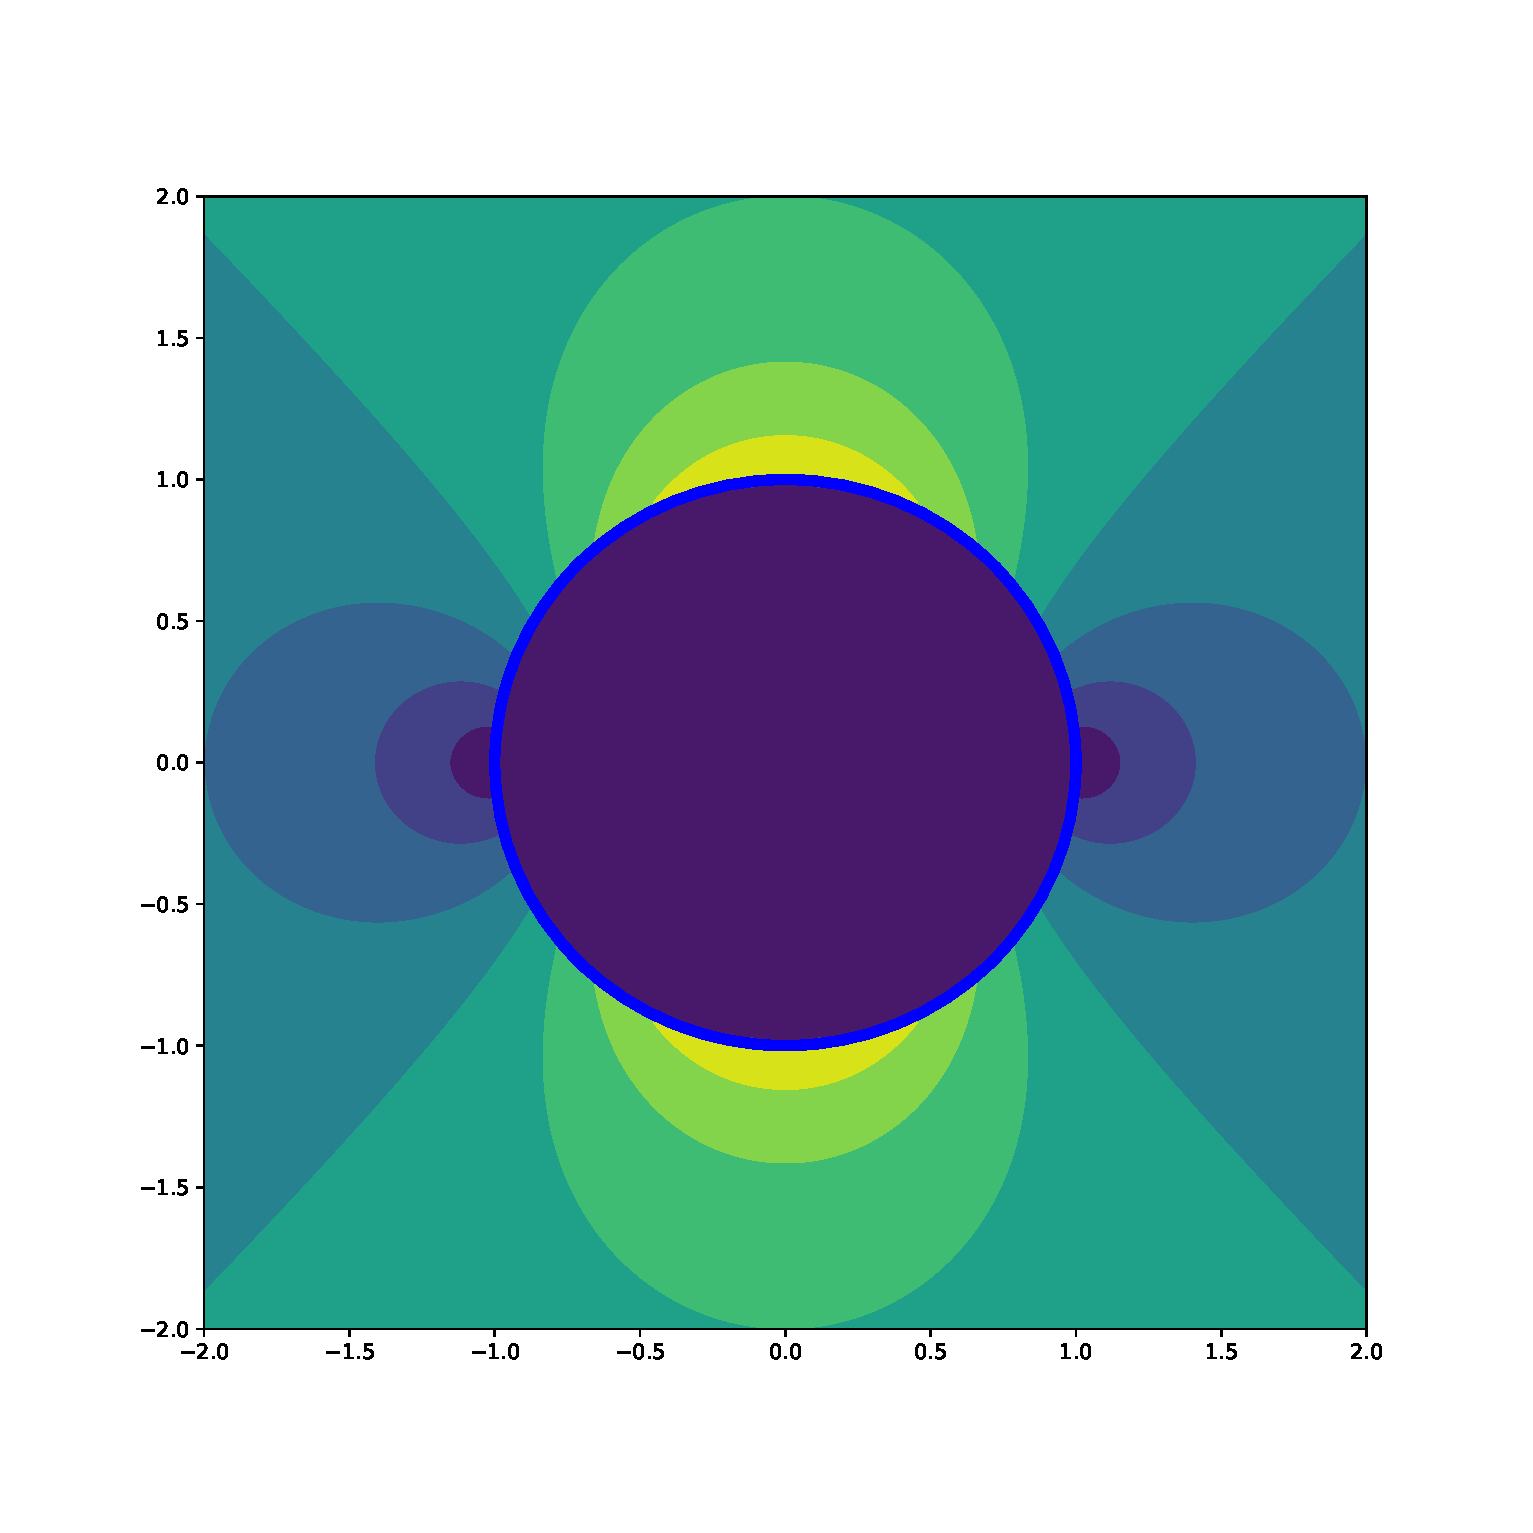
\includegraphics[width=0.4\linewidth]{figures/potential_flow_past_cylinder_vel}
  \caption{
  	Potential flow past a cylinder. Velocity magnitude contours, $u/u_0$.
  	\label{fig:potential_flow_past_cylinder_vel}}
\end{figure}


\begin{figure}
  \centering
  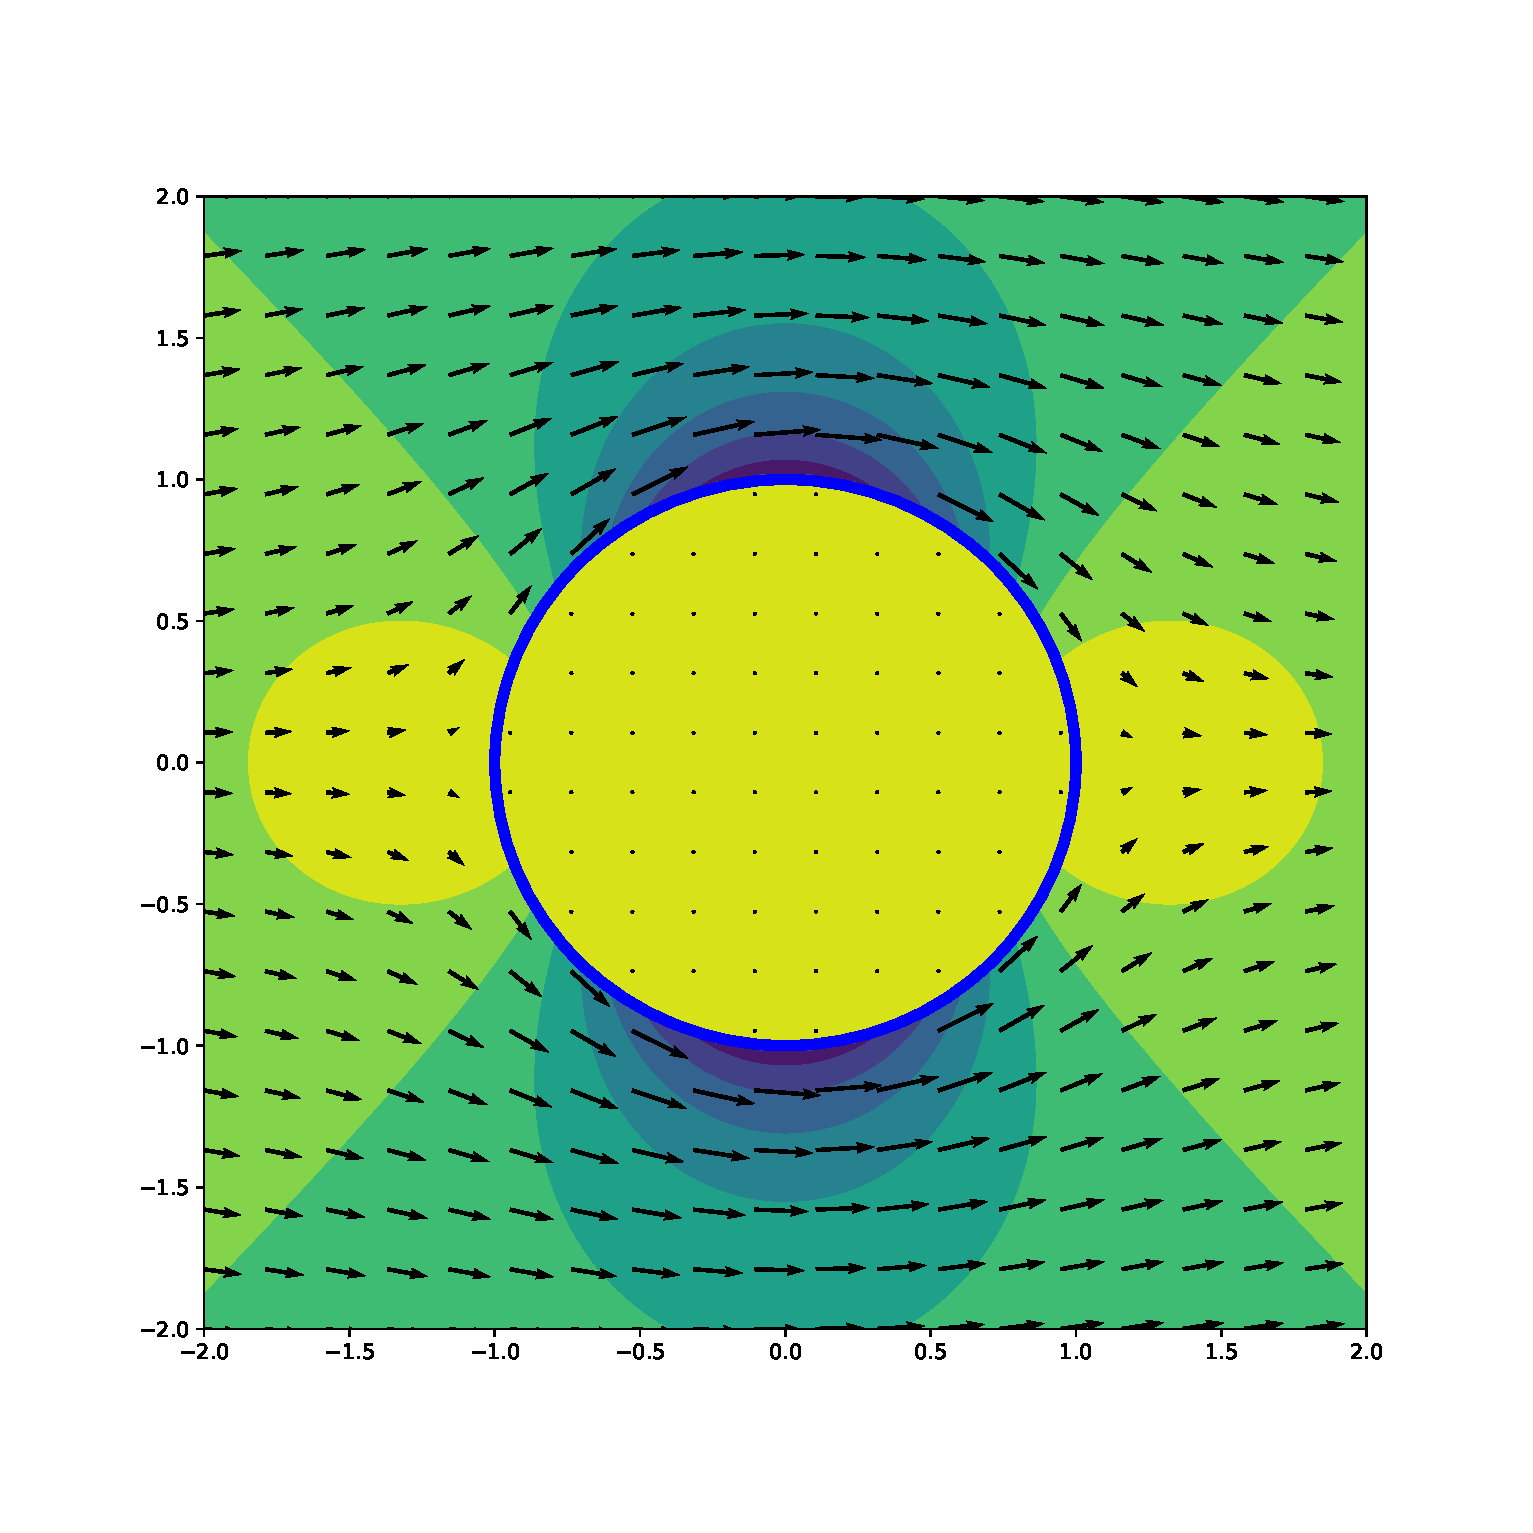
\includegraphics[width=0.4\linewidth]{figures/potential_flow_past_cylinder_vel_p}
  \caption{	Potential flow past a cylinder. Velocity field, $\bfu/u_0$, and pressure field $ (p-p_0)/(\rho u_0^2)$. \label{fig:potential_flow_past_cylinder_vel_p}}
\end{figure}


The pressure field can be obtained from Bernoulli's principle:
%
\begin{equation*}
p = p_0 +  \frac{\rho}2  \left(u_0^2 - u^2 \right)  ,\\
\end{equation*}
so it basically resembles the velocity modulus above, but for
a non-important constant shift, and multiplication by $-\rho/2$.
Isobars are plotted in Fig. \ref{fig:potential_flow_past_cylinder_vel_p}, together
with the velocity field. It is clear that the velocity field does not simply ``goes from high to low pressures''.
To make this point clearer, Figure \ref{fig:potential_flow_past_cylinder_phi_p} 
shows isobars and contours of the potential field, to stress the difference between the
two, except in those areas in which the two fields happen to
have similar gradients.

\begin{figure}
  \centering
  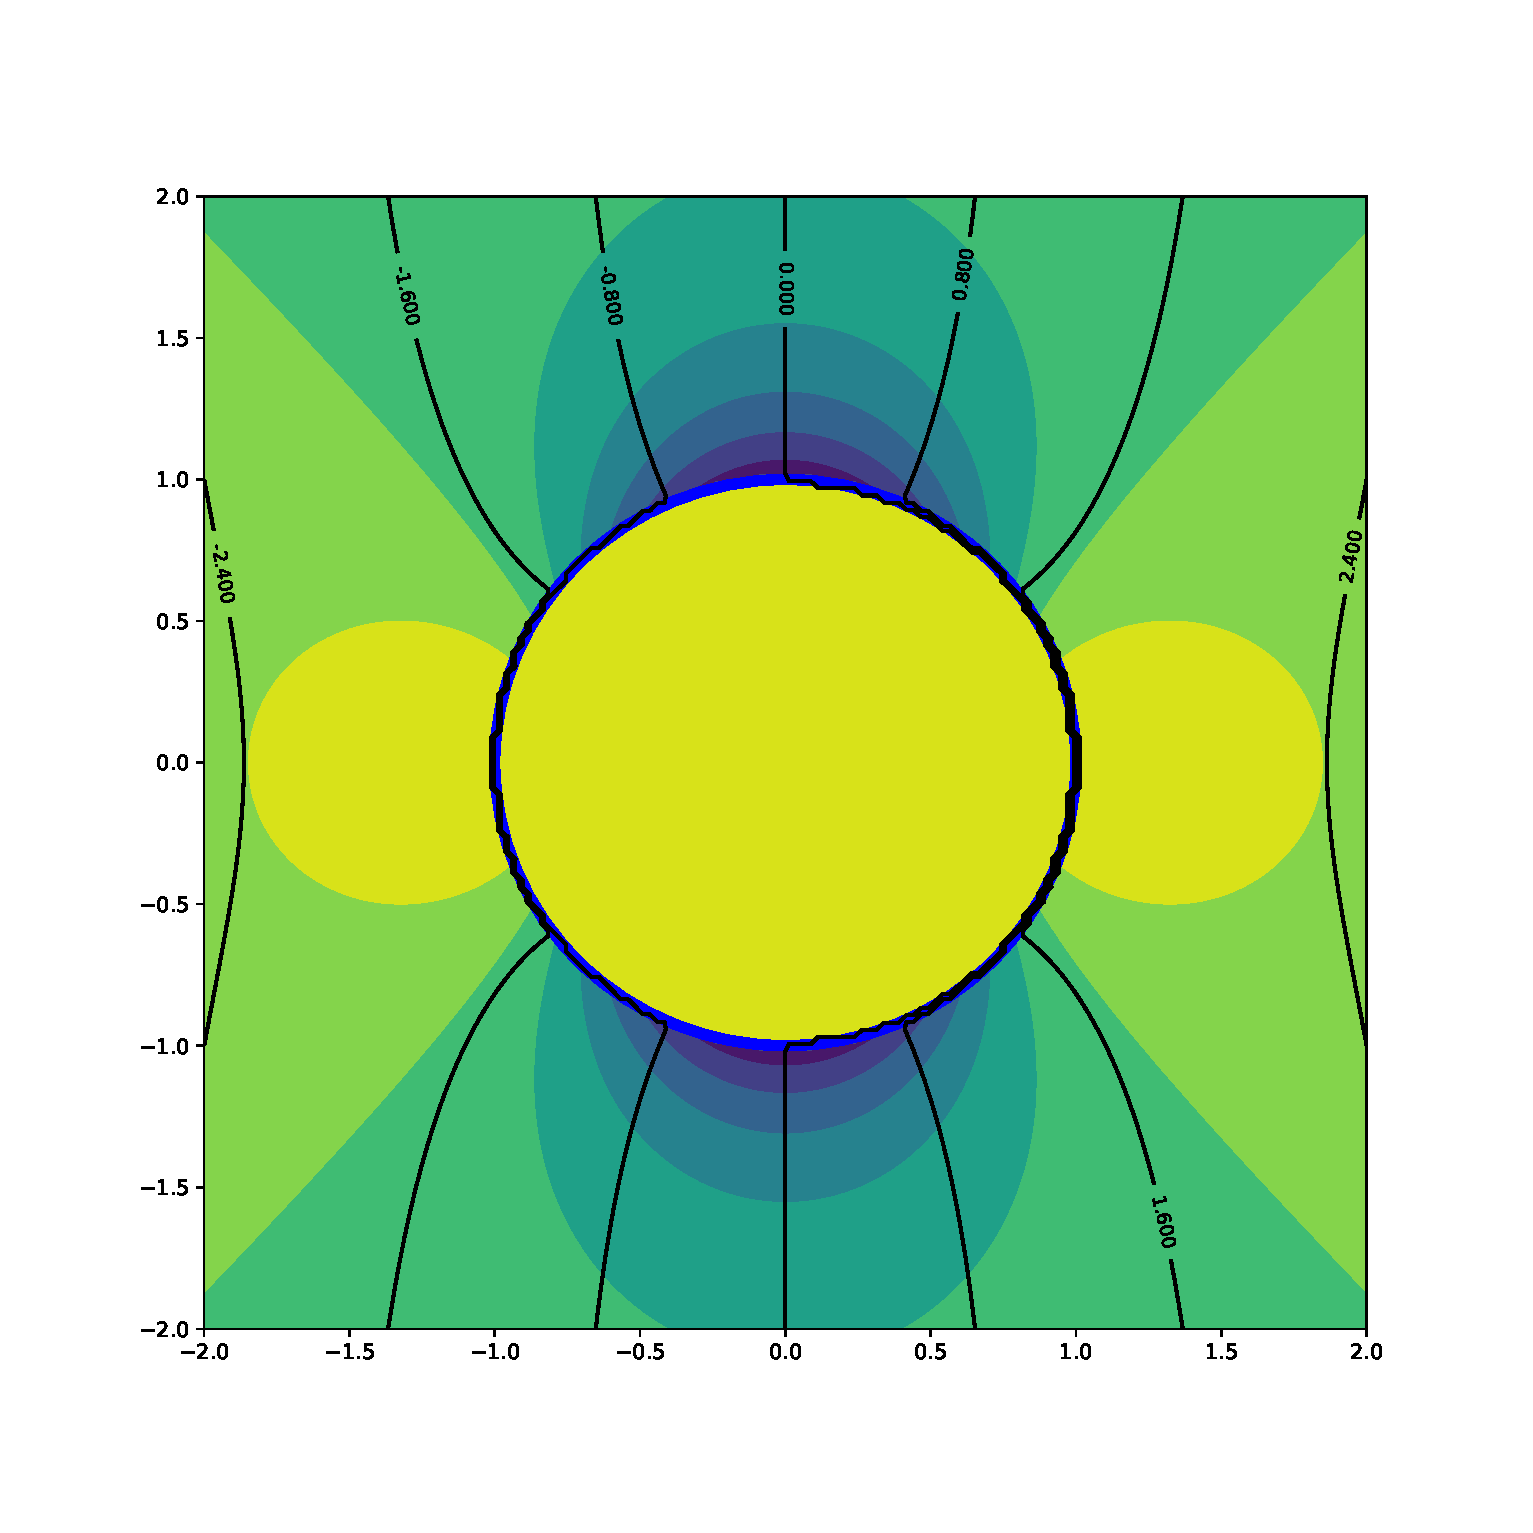
\includegraphics[width=0.4\linewidth]{figures/potential_flow_past_cylinder_phi_p}
  \caption{	Potential flow past a cylinder. Pressure field $ (p-p_0)/(\rho u_0^2)$
  and potential $\phi / (u_0 R)	$ .
  	\label{fig:potential_flow_past_cylinder_phi_p}}
\end{figure}

The pressure field has a striking left-right symmetry. This of course
applied to its value at the surface. Since the pressure is the only
force this fluid may exert upon the cylinder, the consequence is that
the net force on it is exactly zero. The push it experiences towards
the right is exactly cancelled by the push back towards the
left. Therefore, the drag, which in this case is the net horizontal
force, is zero.

This striking result is known as d'Alembert's paradox, and marked a
historical chasm between theoretical fluid mechanics and applied
hydraulics. Indeed, the applied community could accept that the push
back may exist. Indeed, it had been hypothesized to be solely
responsible for objects moving even when not given a force in
Aristotelian physics. The effect is real, and is used regularly by
cyclist that may take advantage from it, by staying close to the back
of a moving vehicle. However, it is not acceptable to accept that it
should be exactly equal to the drag.

We now know that the crucial ingredient is the viscosity, which
manifests mathematically in a different boundary condition, such as
no-slip. This way, a real cylinder is dragged with the flow. We will
show later that it is easy to obtain the drag on a sphere in the limit
of high viscosity (a cylinder is not solvable due to another paradox,
as we will see.)

In case some mathematical justification is required, the pressure
at the surface on the cylinder is
\begin{equation}
  \label{eq:press_at_cyl_pot}
  p=   p_0  + \rho  u_0^2  \left[ \frac12 - \cos(2\theta)  \right] ,
\end{equation}
as plotted in Figure.


\begin{figure}
	\centering
	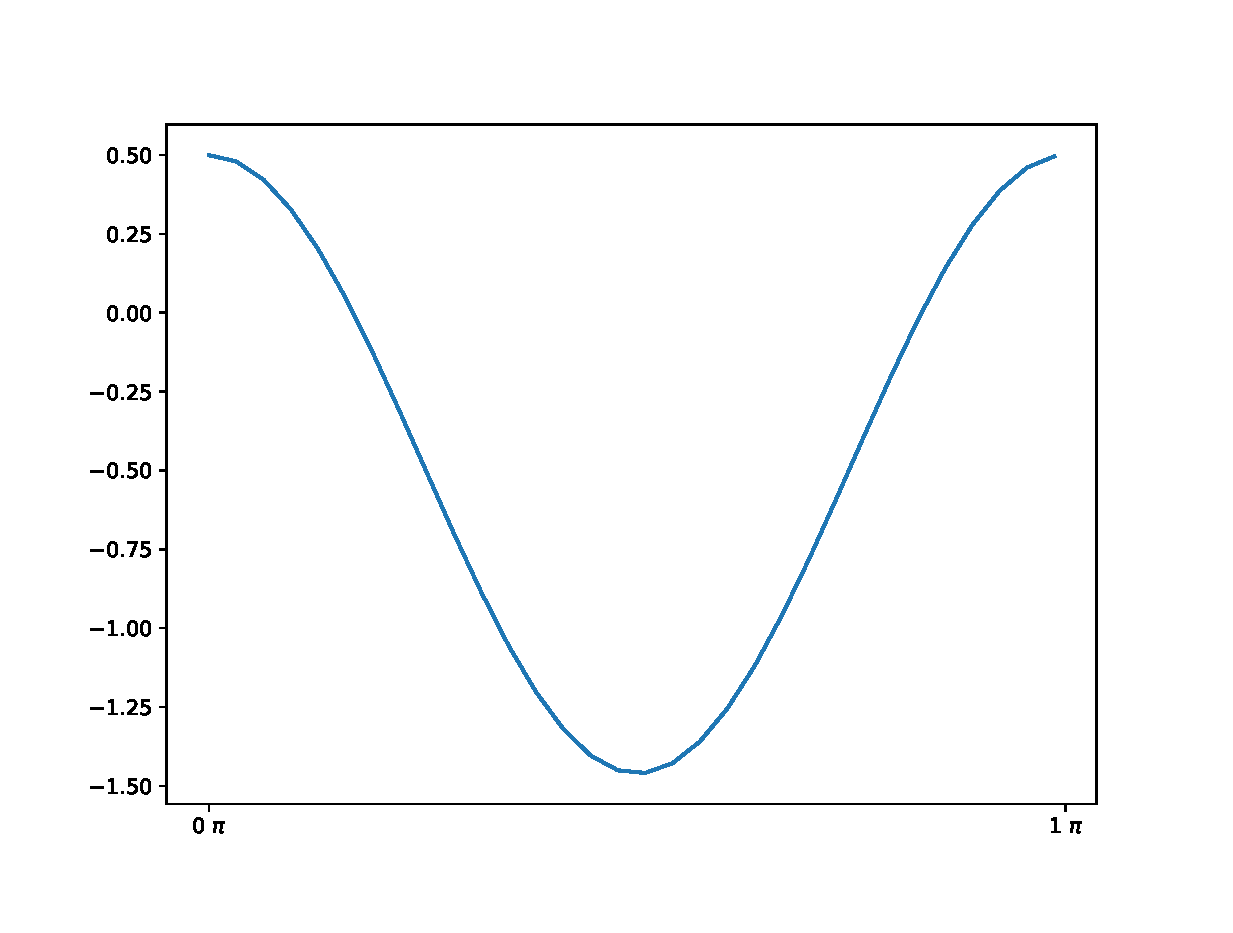
\includegraphics[width=0.7\linewidth]{figures/potential_flow_past_cylinder_p_on_cyl}
	\caption{Potential flow past a cylinder. Pressure on
		cylinder surface $ (p-p_0)/(\rho u_0^2)$. Position $0$ corresponds to the
	``stern'' of the cylinder, position $\pi$ to the ``bow''.   }
	\label{fig:potential_flow_past_cylinder_p_on_cyl}
\end{figure}



%In the last equation, the identity
%$\sin^{2}\theta ={\frac {1-\cos(2\theta )}{2}}$ has been used.

Now, the drag is given by the net force in the $x$ direction. The
(vector) force due to pressure is:
\[
\mathbf{F} = \int_0^H \int_0^{2\pi}   p(\theta)  \bfn  R d\theta  dz ,
\]
where $p(\theta) \bfn \bhe_x R d\theta dz $ is the pressure force on a
differential surface of area $ R d\theta dz$. Now, the drag will be
its projection on the horizontal axis:
\[
D= \mathbf{F} \cdot \bhe_x = \int_0^H \int_0^{2\pi}
p(\theta) \cos(\theta) R d\theta dz .
\]
The integral is zero, since it consists of two terms. The first one
involves constant term. Of course, a constant pressure exerts no net
force, and mathematically:
\[
 \int_0^{2\pi} C \cos(\theta) d\theta = C  \int_0^{2\pi}  \cos(\theta) d\theta = 0 .
\]

The other term involves a $\cos(2\theta)$ term. Now, this integral is also
zero:
\[
 \int_0^{2\pi}  \cos(\theta)  \cos(2 \theta) d\theta = 0 .
\]
The reason is that cosines form an
orthogonal basis: an integral of two different cosines over one period
will be zero --- unless they are the same cosine, when the integral is
$\pi$. To be precise, for integer $m$ and $n$:
\[
\frac{1}{2\pi} \int_0^{2\pi}  \cos(m \theta) \cos(n \theta)  d\theta = 
\begin{cases}
0 \quad \text{if } m\ne n \\
\frac12 \quad \text{if } m = n 
\end{cases} .
\]
(It is more elegant to divide by $2\pi$ to express the integral as a
mean value.) In fact, the previous result about constant pressure
is a particular case in which $m=0$.

It is also interesting that similar integrals involving a sine and a
cosine are always zero (i.e. sines are cosines are orthogonal.)
This shows that the lift is always null:
\[
L= \mathbf{F} \cdot \bhe_x = \int_0^H \int_0^{2\pi}
p(\theta) \sin(\theta) R d\theta dz = 0
\]



\subsection{Streamlines}

For steady 2D flow, it is very convenient to introduce the stream
function $\psi$. It is defined such that its contour lines produce the
streamlines \index{streamline}, i.e. the lines the fluid particles
trace as they move. Upon some reflection, this means that its gradient
should always be perpendicular to the velocity:
\begin{equation}
  \label{eq:stream_perp_to_u}
  \bfu \cdot \nabla\psi = 0 .
\end{equation}
In steady flow, this means $d\psi/dt=0$, so the value of $\psi$ is
carried with the flow. This is at variance with the potential, whose
gradient is parallel to the velocity (it is indeed, the velocity
itself). Thus $\phi$ and $\psi$ are orthogonal functions, in the sense
that their gradients are.

The streamlines are important to visualize flows, in much the same way
as Faraday's field lines are for electromagnetic fields
(mathematically, they are equivalent). In computational fluid
dynamics, they are customarilly computed and plotted, by ``seeding''
points and integrating their motion following the velocity field.  A
fine point is that for unsteady flow, these streamlines are in general
different from the actual trajectories of fluid particles, which are
called ``pathlines'' \index{pathline}.


For steady flow, it is often convenient to define a vector potential
\index{vector potential} in much the same way as it is done for the
magnetic field in electromagnetism:
\begin{equation}
  \label{eq:vector_potential}
  \bfu = \nabla\times \bfA .
\end{equation}

The resulting velocity field will always be incompressible, since the
divergence of a curl is zero.

In the case of 2D, the choice for this vector potential is
\begin{equation}
  \label{eq:A_psi_2D}
  \bfA = \psi(x,y) \bhe_z ,    
\end{equation}
perpendicular to the plane, but dependent on the in-plane
coordinates. With this expression,
\begin{align*}
  u_x &=  \frac{\partial \psi}{\partial y} \\
  u_y &= -\frac{\partial \psi}{\partial x} ,
\end{align*}
and it is easy to check that this stream function indeed traces
stream-lines, since it complies with \ref{eq:stream_perp_to_u}.

In cylindrical coordinates \cite{wiki:del},
\begin{align*}
u_r &= \frac1r \frac{\partial \psi}{\partial \theta} \\
u_\theta &=   - \frac{\partial \psi}{\partial r} .
\end{align*}


\subsection{Streamlines around the cylinder}

With the latter expression for the stream function, and from our
results for the velocity field, the $\psi$ field is found to be

\begin{equation}\label{eq:streamlines_past_cylinder}
\psi = u_0 \left( r-{\frac {R^{2}}{r}}\right)\sin \theta .
\end{equation}
This method, of course, is working backwards from the known
solution. It is also possible to derive the velocity field from the
fact that $\psi$ satisfies Laplace's equation, plus the appropriate
boundary conditions, in a manner very similar to what has been done
for the potential (see Exercise \ref{ex:u_from_psi_cylinder}).

The streamlines, which are the contour lines of this field are shown in
Fig. \ref{fig:potential_flow_past_cylinder}.




\begin{figure}
  \centering
  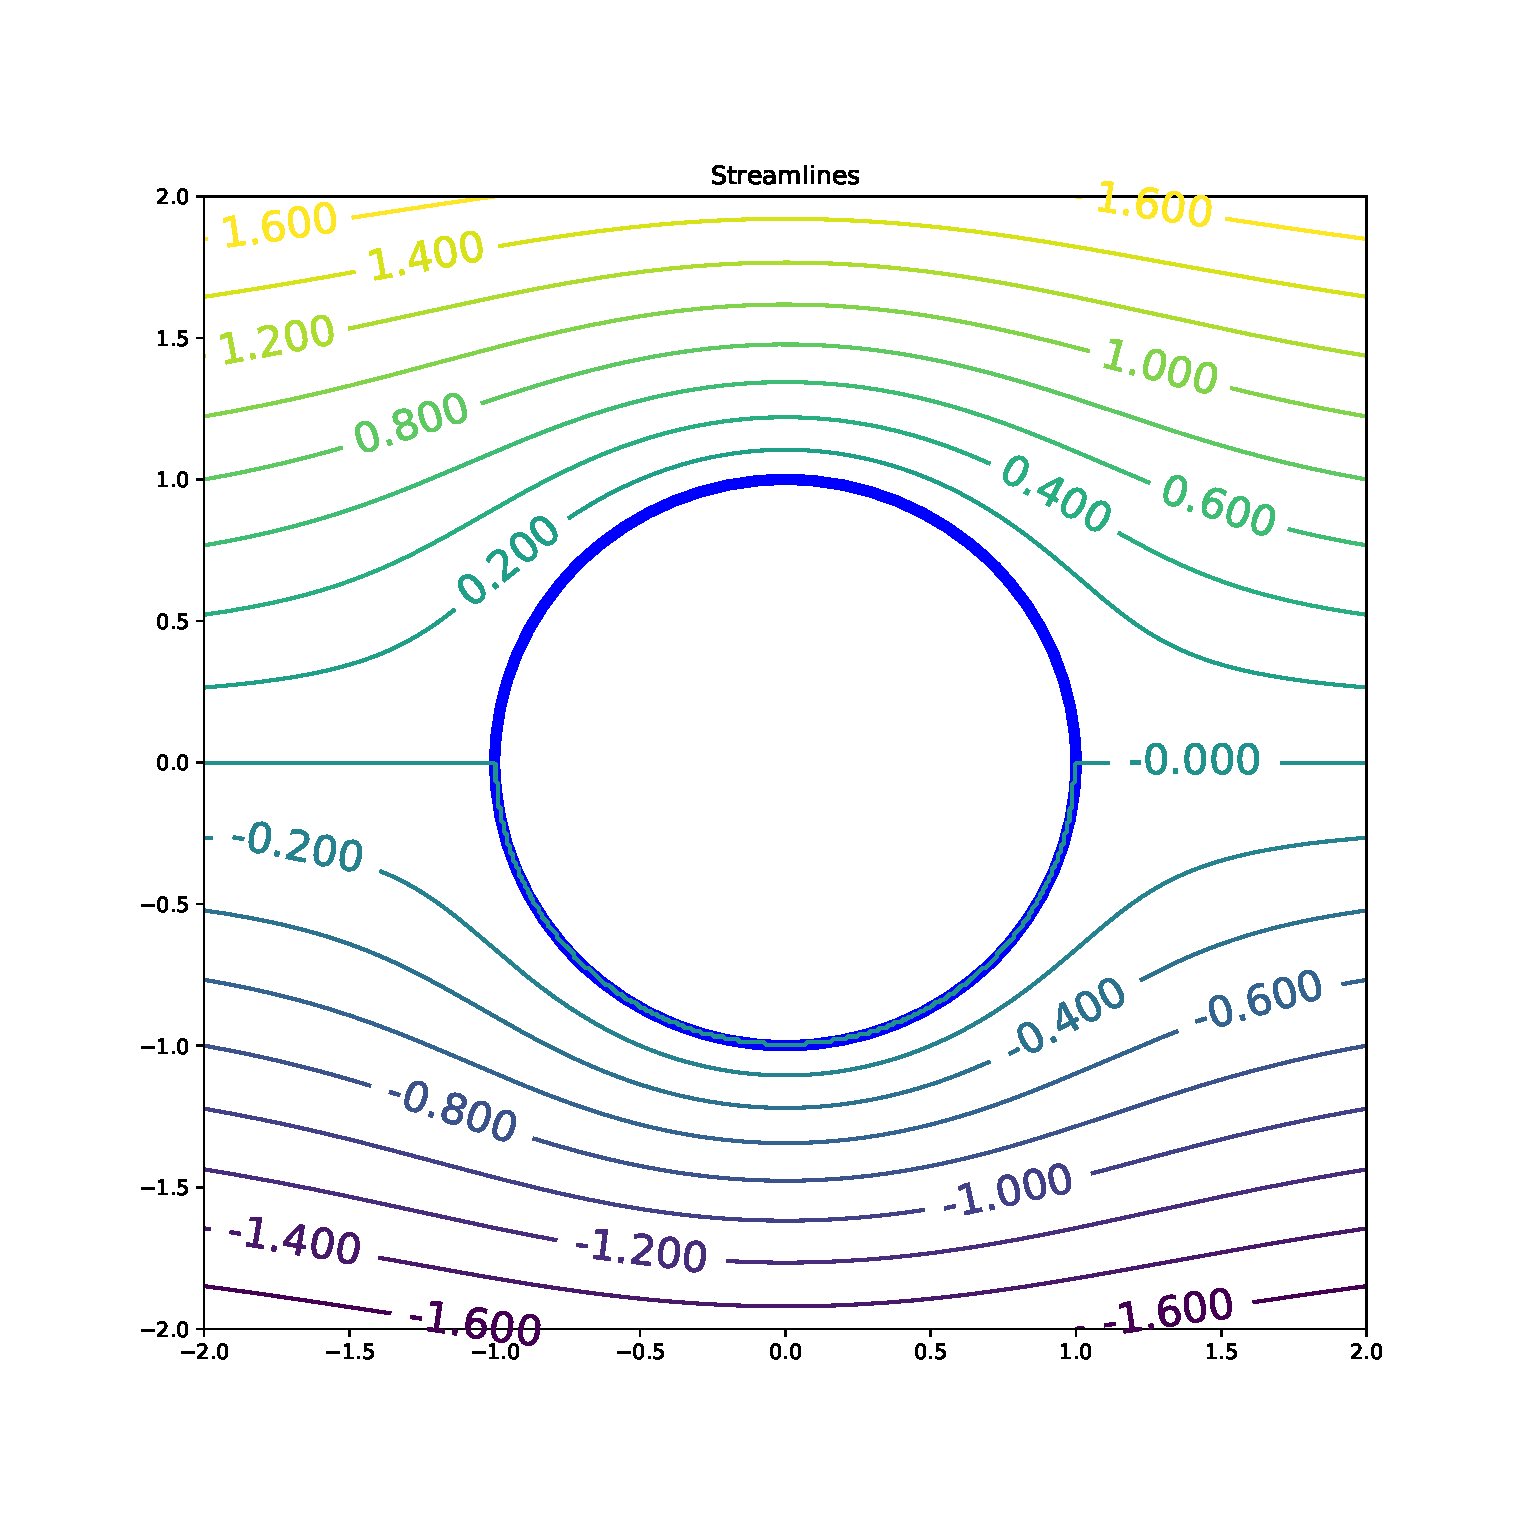
\includegraphics[width=0.6\linewidth]{figures/potential_flow_past_cylinder}
  \caption{Potential flow past cylinder, streamlines
  	as contour lines of function $\psi / (u_0 R)$.
  	\label{fig:potential_flow_past_cylinder}}
\end{figure}

%It is simple and interesting to inquire the form of the streamlines if we were moving with the 
%far-away velocity $\bfu_0$. This would entail subtracting the far-away term, $u_0 r \sin\theta$, %from the stream function \ref{eq:streamlines_past_cylinder}. The resulting streamlines
%are shown in \ref{fig:potential_flow_past_cylinder_moving}. The cylinder is seen to
%``push away'' the surrounding liquid which, nevertheless, comes around and ends up pushing
%against it. This is a further indication of the d'Alembert paradox.

%\begin{figure}
%	\centering
%	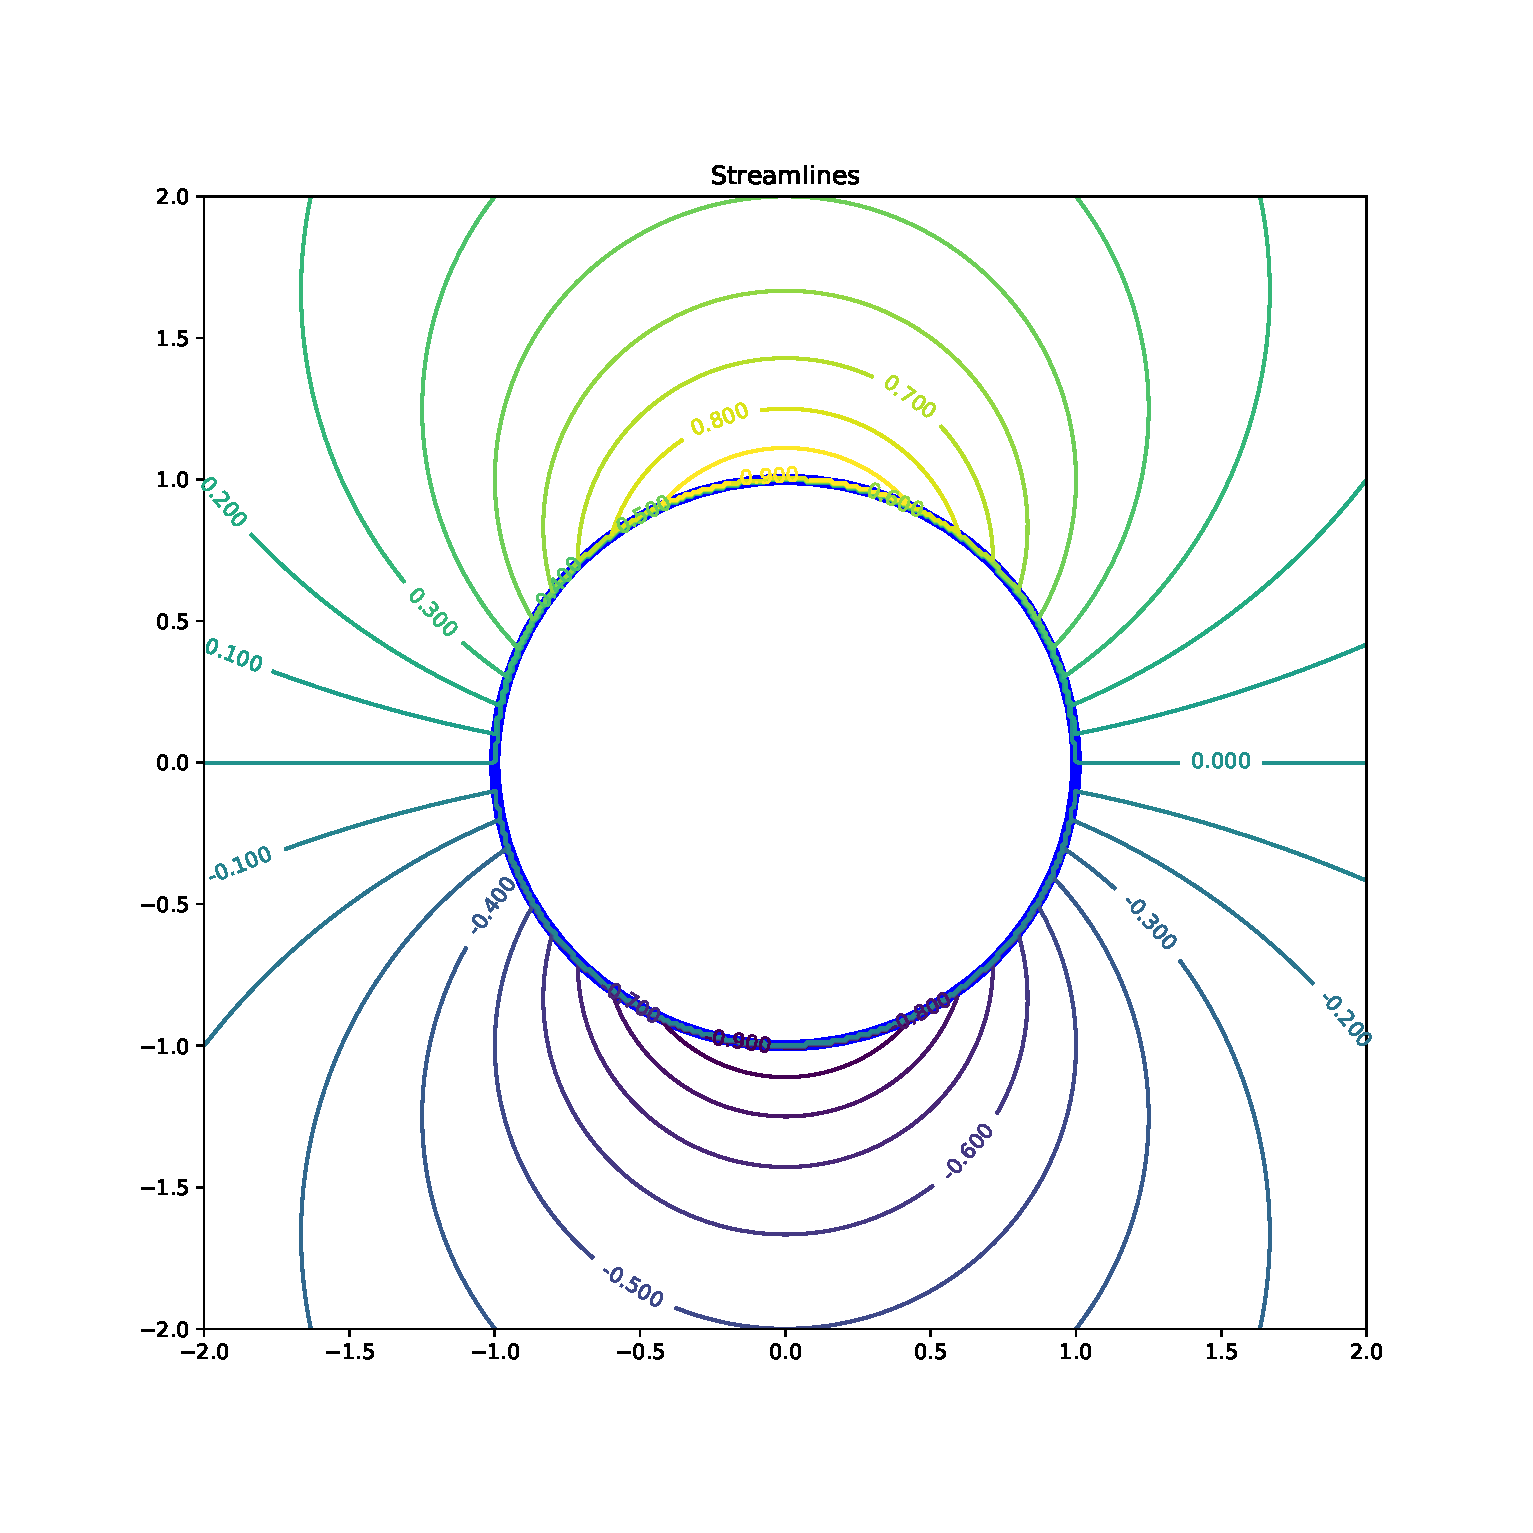
\includegraphics[width=0.6\linewidth]{figures/potential_flow_past_cylinder_moving}
%	\caption{%
%		Potential flow past cylinder, streamlines as seen from the
%		fluid,  contour lines of function $ ( \psi - u_0 r\sin\theta )  / (u_0 R)$.
%	\label{fig:potential_flow_past_cylinder_moving}}
%\end{figure}




\subsection{Potential function, stream function and complex analysis}

Interestingly, the $\psi$ field is also a solution of Laplace's
equation, $\nabla^2 \psi=0$, as can be checked explicitely --- but
also from the identity for the curl of the curl
\cite{wiki:Vector_calculus_identities}:
\begin{equation}
  \label{eq:curl_of_curl}
  \nabla \times \left(\nabla \times \bfA \right)=
  \nabla (\nabla \cdot \mathbf {A} )-\nabla^2\bfA .
\end{equation}

Then, since the velocity field is curl-free:
\begin{equation}
  \label{eq:if_no_curl_then_stream_harmonic}
  0 = \nabla \times \bfu =
  \nabla (\nabla \cdot \mathbf {A} )- \nabla^{2}\mathbf {A} =
  - \bhe_z \nabla^{2} \psi,
\end{equation}
where we use the fact that the $\bfA$ field of \ref{eq:A_psi_2D} is
divergence-free.


There is also the intriguing fact that we may write
\[
\phi = u_0 \Re \left( z  + \frac{R^2}{z} \right) ,
\]
where $z=r e^{i\theta}$ is the complex number related to the $r$ and
$\theta$ coordinates. Then,
\[
\psi = u_0 \Im \left( z  + \frac{R^2}{z} \right) .
\]
%
I.e. both fields are the real and imaginary part of the same complex
function:
\[
f(z) = u_0 \left( z  + \frac{R^2}{z} \right)
\]

This is no coincidence, but a consequence of Cauchy-Riemann
equations: the real and imaginary part of a complex function are
harmonic (i.e. they satisfy Laplace's equation) and orthogonal. To be
more precise, the complex function must be analytic. The later
requirement is pretty general: it means the function must be
single-valued and and must have a derivative everywhere. The reader
may worry about the $1/z$ function blowing up at the origin. This is, however,
\emph{outside} our domain, which ends when $r>R$. The fact that our
domain has this ``hole'' in it has some other consequences, as we will see
next.


\subsection{Circulation and lift}

It turns out that, despite our previous claims of having found the
solution to the problem, this is not a unique solution%
\footnote{This is because our domain has a hole in it. Technically, it
  is not simply-connected. This means there is an additional parameter
  to fix the most general solution. This is called the ``winding
  number'', and is basically this section's $\Gamma$.}.
%
The most general one is given by
\[
 f(z) = u_0 \left( z + \frac{R^2}{z} \right)
 + \frac{i \Gamma}{2\pi} \log z \qquad
 \phi=\Re(f) \quad
 \psi=\Im(f) .
\]
I.e. we may add an additional term which is also analytic.%
\footnote{To be precise, it is not, since $\log z$ blows up at
the origin. But, as with $1/z$ before, the origin is not part of
our domain.}
The $i \Gamma/(2\pi)$ factor is chosen for convenience, as will become
clear. Both $\phi$ and $\psi$ are still harmonic and orthogonal, since
$\log(z)$ is analytic. Notice $i \log(z)= i \log(r) - \theta$, so
$\phi$ contains a term that is just the polar angle, while $\psi$ will
include a $\log(r)$ term.

The resulting velocity field still complies with the boundary
conditions, since the resulting velocities:
\begin{align}
u_r     &=   u_0  \left[ 1 - \left( \frac{R}{r}\right)^2 \right] \cos(\theta) \\
\label{eq:u_theta_cyl_pot_circ}
u_\theta &=   u_0  \left[ 1 + \left( \frac{R}{r}\right)^2 \right] \sin(\theta) +\frac{\Gamma}{2\pi r} 
\end{align}
have an additional term which dies away far from the cylinder, while
the no-trespass condition at the surface is still respected (since the
radial velocity does not change at all).

The name of $\Gamma$ is ``circulation'', since
\[
\Gamma = \oint_C \bfu\cdot d\mathbf{l}
\]
for any contour around the cylinder.%
\footnote{This makes the velocity
  field non-conservative, which is again allowed due to the domain
  being not simply-connected.}

At the surface of the cylinder,
\begin{equation}\label{eq:u_surface_cyl_pot_circ}
	u= u_\theta =  2 u_0  \sin(\theta) +\frac{\Gamma}{2\pi R} .
\end{equation}
The stagnation points then move away from their positions, to points given by
\begin{equation}\label{eq:u_stag_cyl_pot_circ}
	\sin(\theta_\mathrm{st})  = -\frac{\Gamma}{4\pi R u_0} .
\end{equation}
This has two solutions, of course, symmetrically located about the vertical axis.
Notice that the minus sign means that the
stagnation point will be below the horizontal axis for positive
circulation. For values as the right-hand side above $1$ or below $-1$,
the points coalesce into a single stagnation point that is outside the cylinder.

\begin{figure}
  \centering
  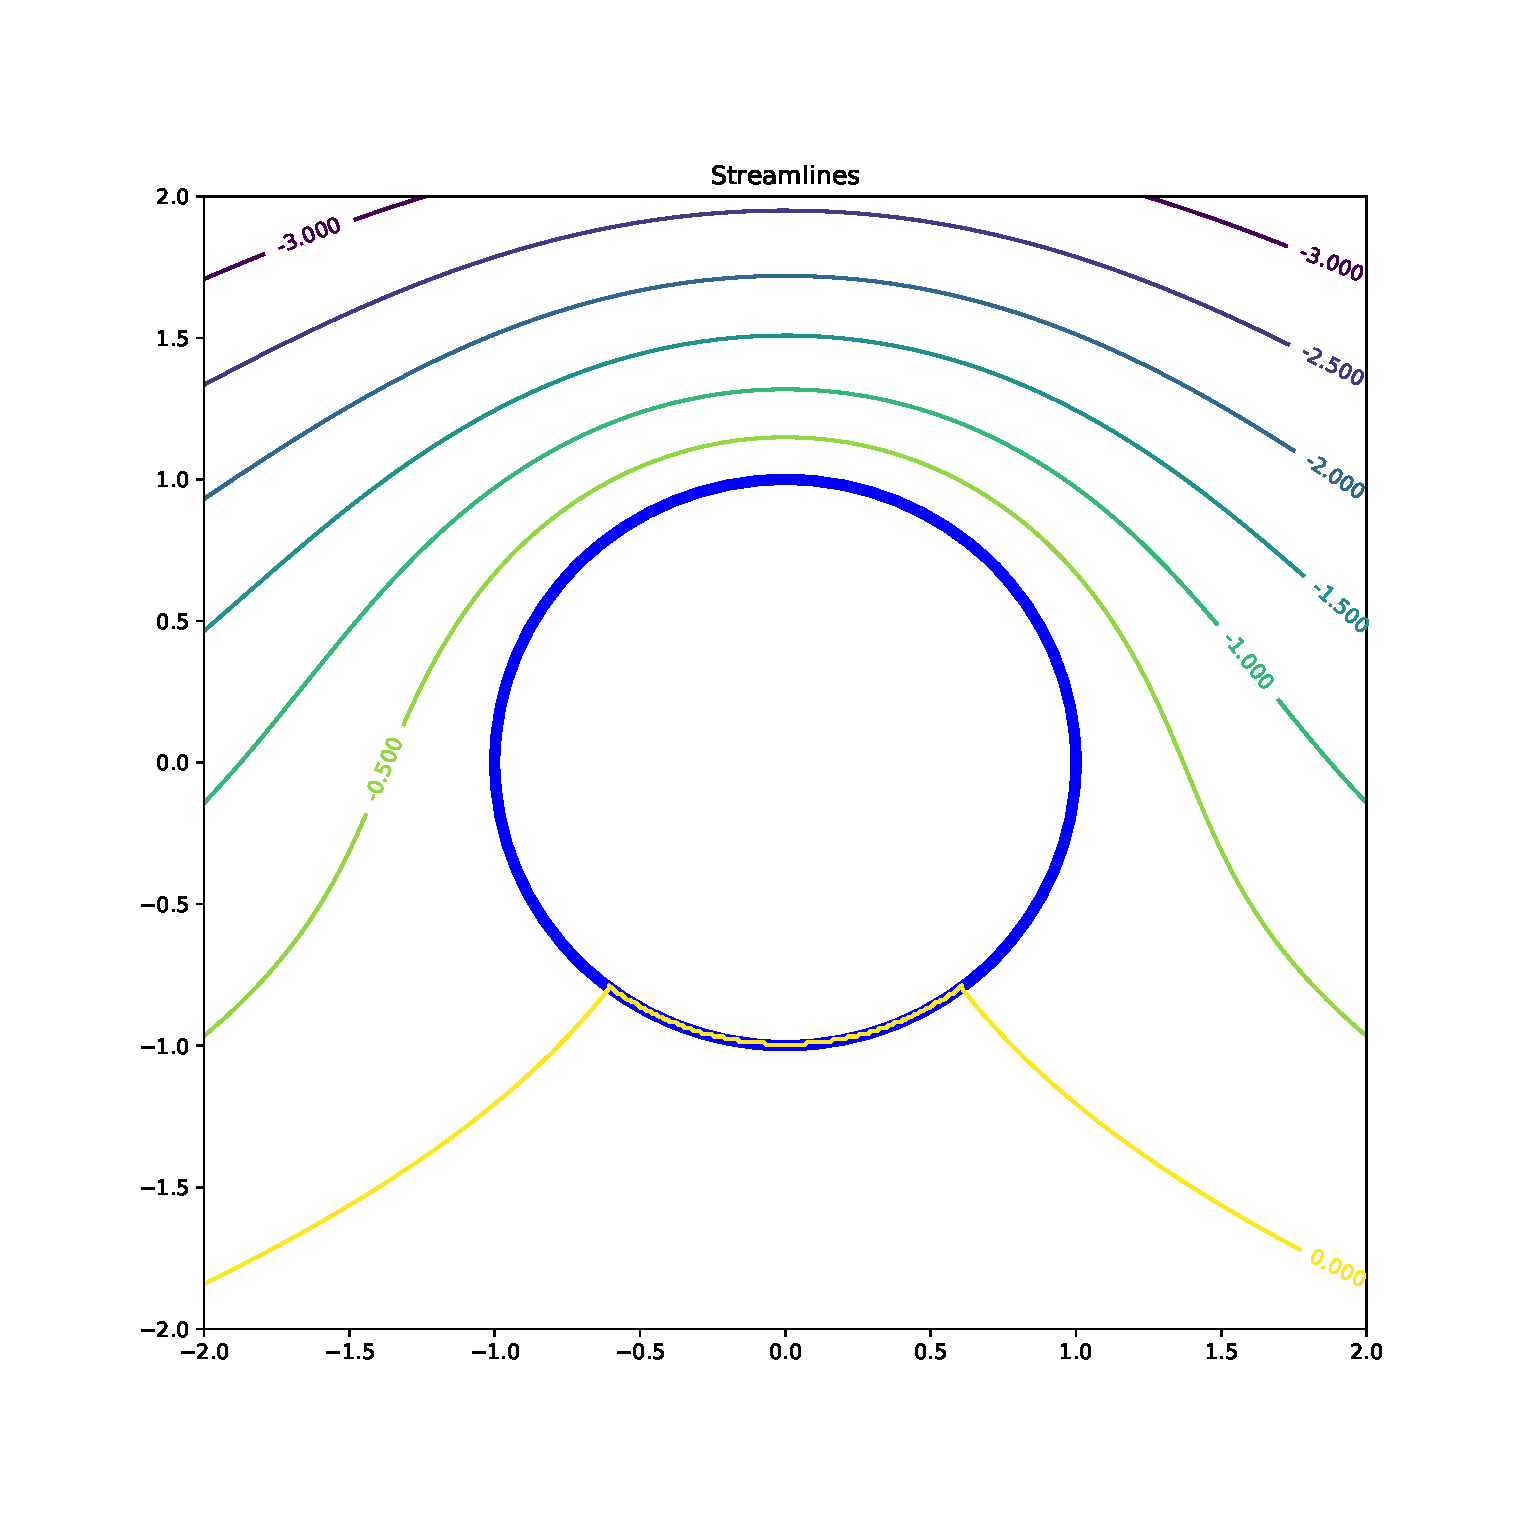
\includegraphics[width=0.4\linewidth]{figures/potential_flow_past_cylinder_rotating}
  \caption{\label{fig:potential_flow_past_cylinder_rotating}}
\end{figure}


This new velocity field does not solve d'Alambert's paradox, but it
does provide a lift, since the pressure at the surface is
\[
p= p_0 + \frac{\rho}2   \left(u_0^2 -  \left[ 2  u_0 \sin(\theta) - \frac{\Gamma}{2\pi R} \right]^2 \right) =
\ldots  2 \rho u_0   \frac{\Gamma}{2\pi R} \sin\theta ,
\]
where we single out the only term that can produce a contribution to the lift.

Now,
\begin{equation}
  \label{eq:lift_potential_cyl}
  L= \mathbf{F} \cdot \bhe_x = \int_0^H \int_0^{2\pi}
  p(\theta) \sin(\theta) R d\theta dz =
  2 L  \rho u_0  R  \frac{\Gamma}{2\pi R}   \int_0^{2\pi}  \sin^2(\theta) d\theta =
  H \rho u_0   \Gamma .
\end{equation}
Therefore, the lift per unit length is $L/H= \rho u_0 \Gamma$. It is
interesting that heavier fluids, high speeds and high $\Gamma$ produce
higher lift forces.

It turns out that this result for the lift is quite general, at least
for these kind of potential flows. It is known as the Kutta-Joukowski
Lift Theorem, and has been used for decades in aeronautics. The idea
is to map our solution for a cylinder to another, more wing-like,
shape, by some conformal transformations. These transformations, or
``mappings'', preserve the harmonicity of functions --- hence the
transformed $\phi$ and $\psi$ will still be solutions of Laplace's
equation. Historically, the best known mappings are the Joukowsky-K\'arm\'an–Trefftz transforms.

For an airplane wing, it makes sense to relate circulation and lift, since
this captures, in a way, the fact that the velocity is higher at the
top of the wing, lower below, so the net circulation is non zero. (Of
course, this cannot hold right at the surface of an actual wing, since
the velocity there will be zero. But this can be measured somewhat
further away, beyond a boundary layer.) The question is, of course,
how to provide an expression for the value of the circulation $\Gamma$.
The historical answer is given by the Kutta condition: at the trailing
edge of the wing, there should be an stagnation point.

The original argument by Kutta actually applies to the velocity being the
same at the two sides of the trailing edge of a wing. This is explained by
the fact that the velocity field should not include discontinuities. In
fact, such a velocity field may be allowed in the Euler equations, but in
an ideal fluid the viscosity, however small, will smear out such jumps. 
In any case, according to our inviscid
solution the velocity is always tangential to the wing. The only
way the velocity can match, coming from opposite sides of the wing, is by
being zero. Thus, the wing geometry fixes the angle $\theta_\text{st}$  on
the cylinder, after a Joukowsky transform. Eq. \eqref{eq:u_stag_cyl_pot_circ}
then implies $\Gamma = - 4\pi R u_0 \sin(\theta_\text{st})$, hence
Eq. \eqref{eq:lift_potential_cyl} yields
\[
L = -4\pi R H  \rho u_0^2 \sin(\theta_\text{st}) =
- 2 A  \rho u_0^2 \sin(\theta_\text{st}) .
\]
with the prediction that the lift force will increase quadratically with speed. In the last equality, we have written $A=2\pi R H$ for the total area of the cylinder, showing a typical result
of a force being equal to the area times a pressure-like
term. The minus sign should not cause concern, since the angles are negative for positive circulation. Notice there is even a prediction of a maximum lift force,
when the sine has a value of $-1$, which is perhaps an indication of the
stalling phenomenon (?).

Another way to fix the value of the vorticity is when the cylinder is supposed
to be rotating with angular velocity $\omega_0$. In this case, lift is generated
by the Magnus effect. This effect is used (for spheres) in sports, such as tennis, golf and
football. Also, for cylinder-like rotors, in ``rotor ships,'' which use
the Magnus effect for propulsion.

We may obtain an expression for the Magnus force by equating the
circulation term $\Gamma/(2\pi R)$ for the tangential velocity
of the fluid at the surface of the cylinder
(Eq. \ref{eq:u_theta_cyl_pot_circ}) with the cylinder surface
velocity:
\[
\frac{\Gamma}{2\pi R} = \omega_0 R 
\]
This is a sort of ``no-slip'' condition --- but, incomplete,
since the correct condition would be the whole tangential velocity
being equal to the cylinder surface velocity, and we are equating
its mean value only. This requirement is, again, too strong for an ideal fluid,
and is only met when viscosity is introduced.

The expression for the Magnus force is then,
\[
L = 2 \pi R^2 H \rho u_0 \omega_0  =
A \rho V_0   u_0
\]
proportional to both the wind speed $u_0$ and the angular
velocity of the spinning cylinders, $\omega_0$.
In the last equality we have again introduced the area
of the cylinder, while $V_0 := R \omega_0$ is the velocity
of the cylinder surface.
Since the force is perpendicular
to the wind, the Magnus effect works best for wind coming
from the sides (``abeam''). Also, this is the ``apparent wind'':
the wind at the cylinders is the vector sum of the true
wind and the velocity of the ship. The effect of the latter
is to bring the apparent wind closer to the fore.

As an aside, if we move with the flow velocity $\bfu_0$,
% the airplane, or on the ship,
we will \emph{not} measure those velocity fields. The far-way term
should be avoided in every equation, and the resulting velocity looks different.
This is shown in Fig. \ref{fig:potential_flow_past_cylinder_moving}, for the
flow past a cylinder with and without circulation. It is seen that,
for an observer moving with the flow, a cylinder moving to the left
pushes the surrounding fluid from the fore, which then moves around towards the aft
(where it pushes our vehicle, magically making our journey a cost-less one!).

\begin{figure}
  \centering
  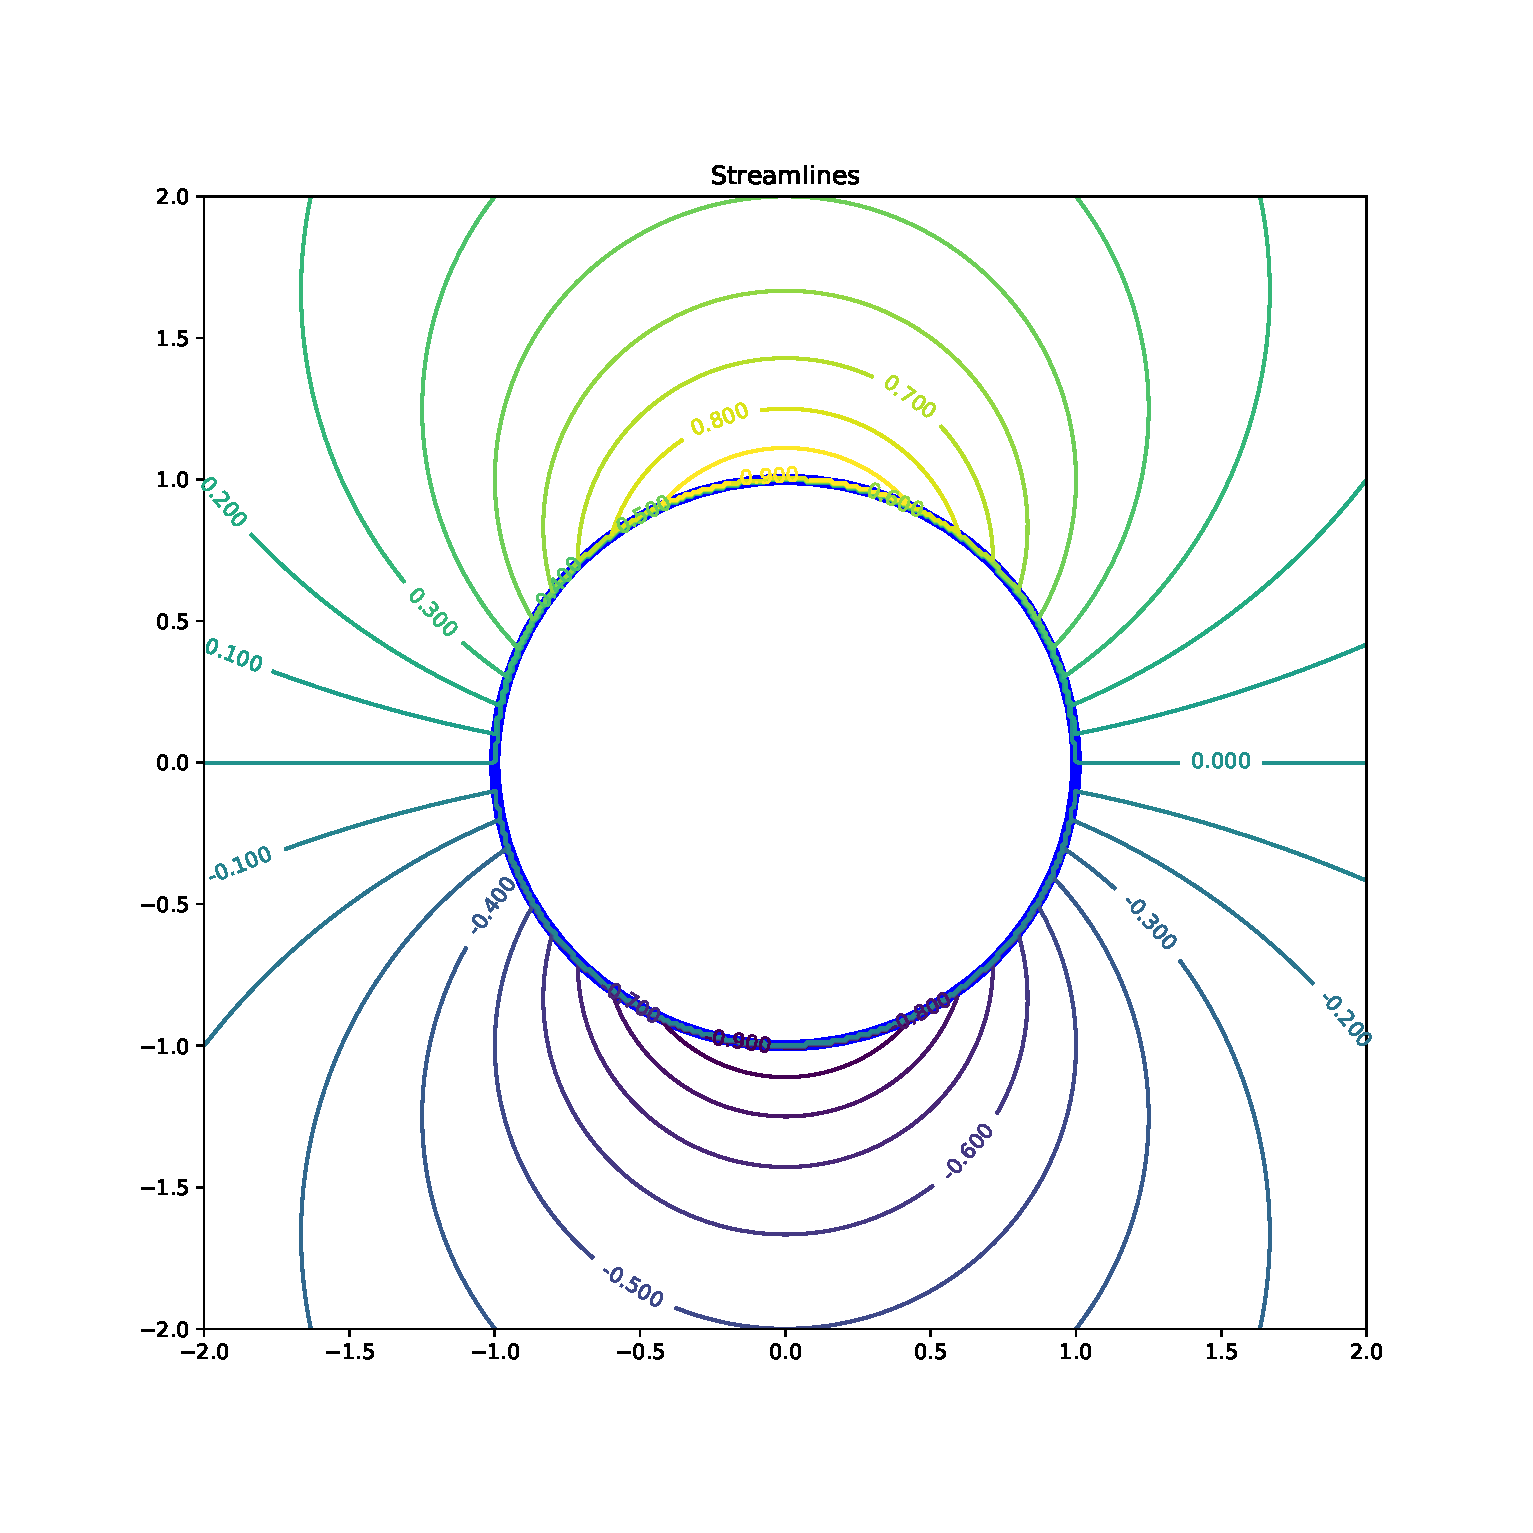
\includegraphics[width=0.4\linewidth]{figures/potential_flow_past_cylinder_moving}
  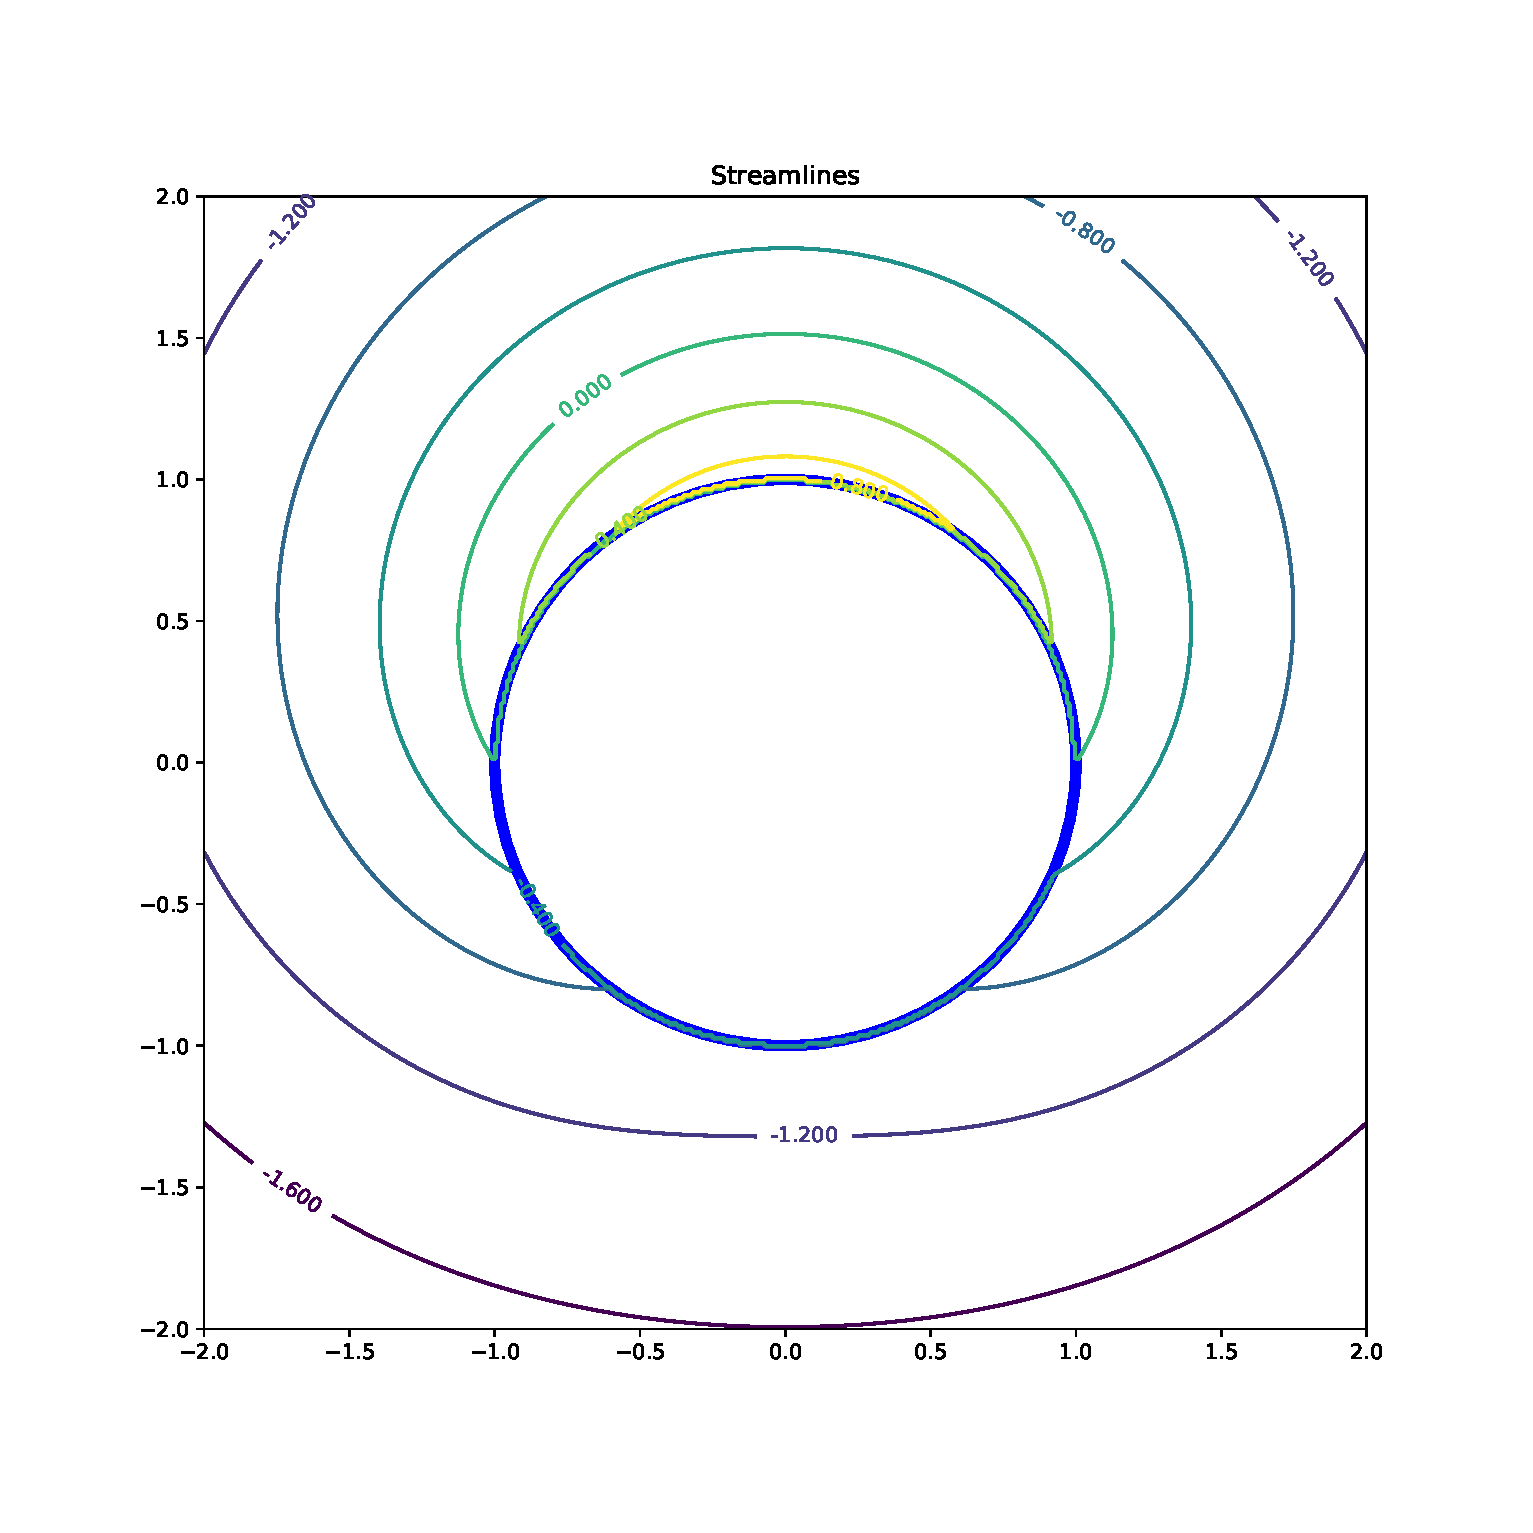
\includegraphics[width=0.4\linewidth]{figures/potential_flow_past_cylinder_rotating_moving}
  \caption{%
  		Potential flow past cylinder, streamlines as seen from the
  		fluid,  contour lines of function $ ( \psi - u_0 r\sin\theta )  / (u_0 R)$.
  	\label{fig:potential_flow_past_cylinder_moving}}
\end{figure}

\subsection{Power and energy}

We may ask ourselves about the power transferred to the fluid, which was discussed in
\S \ref{ss:Euler_energy}. Since the flow is incompressible,
\[
\frac{d \epsilon}{d t} = -\frac{1}{\rho} \bfu \cdot \nabla p .
\]

The pressure is related to the square of the velocity field (by Bernoulli's principle), hence
\[
-\frac{1}{\rho} \bfu \cdot \nabla p =  \frac12 \bfu \cdot \nabla u^2 .
\]
The expression of $u^2$ was given in \eqref{eq:u2_flow_cylinder}, from
which, after some calculations, we find
\[
\frac{d \epsilon}{d t} =
\frac{2 u_0^3 R^3}{r^3}
\left[ 
\cos(3\theta) +
\frac{R^2}{r^2}
\left( \frac{R^2}{r^2} - 2 \right) \cos(\theta)
\right] .
\]

In Fig. \ref{fig:potential_flow_past_cylinder_energy} we show the power
for potential flow around a cylinder. This power is defined as the time variation
of the specific energy $e$. We see there are two zones in the upwind face in which the
fluid would heat up, and two zones in the downwind face where it would cool down. The
overall energy change is null.


\begin{figure}
	\centering
	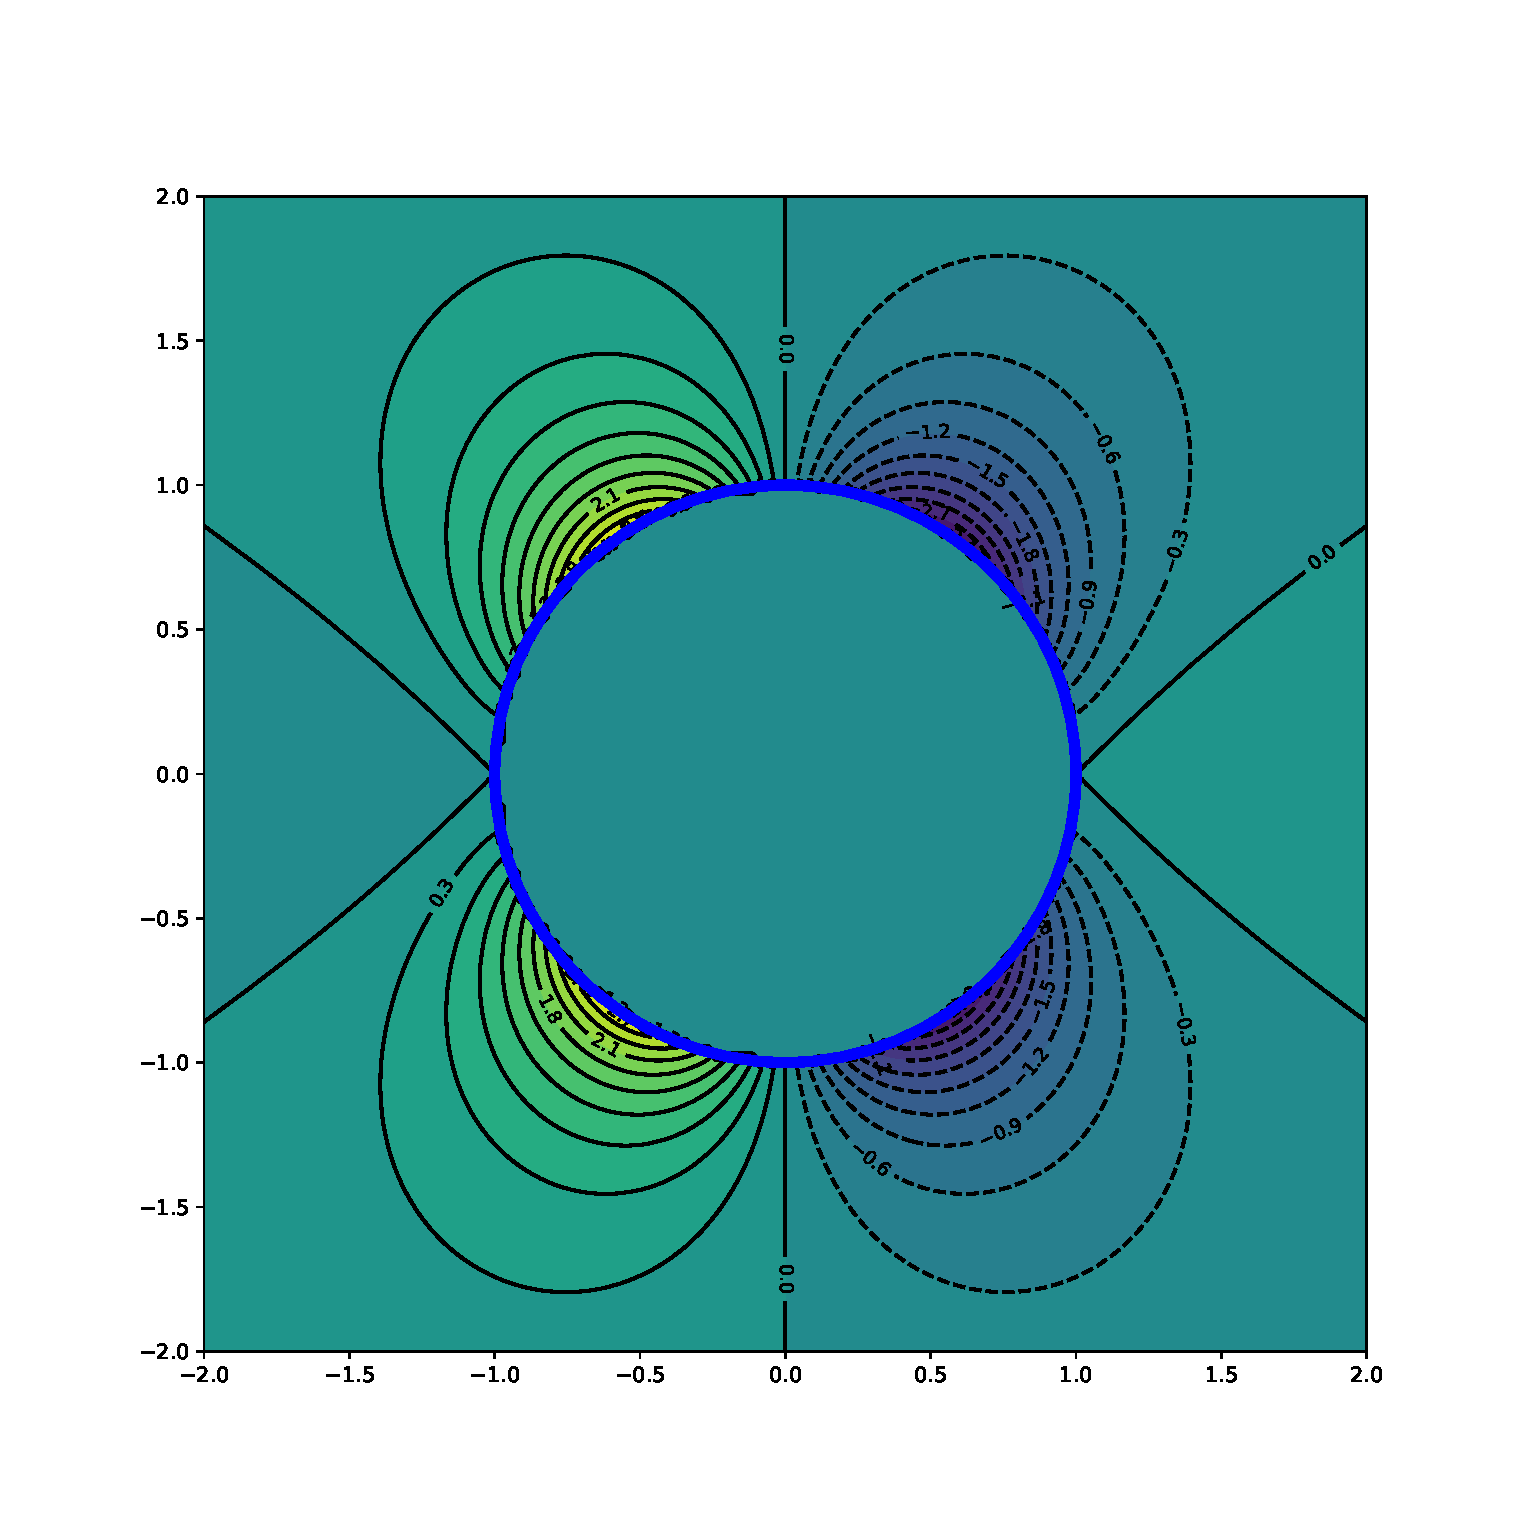
\includegraphics[width=0.4\linewidth]{figures/potential_flow_past_cylinder_power}
	\caption{Specific power (change in specific energy with time) for potential
		flow past cylinder.  \label{fig:potential_flow_past_cylinder_energy}}
\end{figure}



\section{Flow past a sphere}

With the same assumption of potential flow as in the cylinder, the
axisymmetric flow past a sphere may be tackled by using the potential,
which should satisfy Laplace's equation, plus these boundary
conditions:
\[
  \phi (r\to \infty) \to u_0 z = u_0 r \cos\theta \qquad
  u_r(r=R) =\left. \frac{\partial \phi}{\partial r} \right|_{r=R} = 0 .
\]
Spherical coordinates \index{spherical coordinate system} are used:
$r$ is the distance to the origin, $\theta$ is the polar angle (angle
with the $z$ axis), and the azimuthal angle (angle around the $z$
axis), here absent due to symmetry, is $\phi$ %.
\footnote{See \ref{sec:notation} for naming conventions is spherical
coordinates.}.


Similarly to the cylinder, let us try a function
\[
\phi =  \left( u_0 r  + f(r) \right) \cos(\theta)  .
\]

By using the expression of the Laplacian in spherical coordinates
\cite{wiki:del}, we soon come to the conclusion that $f(r)= A/r $ in
order Laplace's equation be satisfied. This function also vanishes as
$r$ gets large, as it should. With the no-trespassing condition for the
velocity the value of $A$ may be found out.

The final result is
\[
  \phi(r,z) = u_0 r
  \left[
    1 +
    \frac12 \left( \frac{R}{r}\right)^3
  \right] \cos\theta .
\]
From its gradient we get the velocity field:

\begin{align*}
u_r &=  u_0
  \left[
    1 -
      \left(\frac{R}{r}\right)^3
  \right] \cos\theta \\
u_\theta &=  -u_0
  \left[
    1 + \frac12
      \left(\frac{R}{r}\right)^3
  \right] \sin\theta
\end{align*}


\subsection{Streamlines past a sphere}

For axisymmetric flows, streamlines may be defined on a plane, since
the resulting flow does not depend on the azimuthal angle (the angle
around the axis of symmetry, which is $z$). However, these are not 2D
flows, and the equations are more involved.

In this case, the velocity field depends only on the other two
coordinates. In spherical coordinates,
\[
  \bfu = \bfu(r,\theta) .
\]

The vector potential may still be thought of as ``perpendicular'' to the other
two coordinates. In spherical coordinates:
\[
  \bfA = A(r,\theta)  \bhe_\phi ,
\]
i.e. it is purely azimuthal. It is also divergence-free, so that is
satisfies Laplace's equation for a curl-free flow, by the argument
exactly as in Eq. \ref{eq:if_no_curl_then_stream_harmonic}.

However, the simple choice of $A=\psi$ will \emph{not} result in the correct
stream-line behavior of Eq.  \ref{eq:stream_perp_to_u}. We must recall
that the contour lines of the streamline function correspond
to the velocity stream lines, as encapsulated in
the requirement $\bfu\cdot\nabla\psi =0$.

By writing the gradient of $\psi$ in spherical coordinates,
\[
\nabla \psi =
{\partial \psi \over  \partial r} \bhe_r +
\frac1r {\partial \psi \over  \partial \theta} \bhe_\theta ,
\]
and the velocity as the curl of the vector potential in spherical coordinates,
\begin{align}
\label{eq:u_from_A_spherical}
u_r = (\nabla\times A)_r    
&=  \frac {1}{r\sin \theta }
\frac{ \partial  \left( A  \sin \theta \right) }{\partial \theta }  \\
u_\theta = (\nabla\times A)_\theta
&= - \frac1{r} \frac{\partial (rA) }{\partial r} ,
\end{align}
the scalar product of both is
\begin{align*}
\bfu\cdot\nabla\psi  =
& \frac{1}{r\sin \theta }
\frac{ \partial  \left( A  \sin \theta \right) }{\partial \theta }
{\partial \psi \over  \partial r} - \\
& -
\frac1{r^2} \frac{\partial (rA) }{\partial r}
{\partial \psi \over  \partial \theta} .
\end{align*}
%
%In axisymmetric flow,
%\[
%  \divu =
%  {1 \over r^2}{\partial \left( r^2 u_r \right) \over  \partial r} +
%  {1 \over r\sin\theta}{\partial \over \partial  \theta} \left( u_\theta\sin\theta %\right) ,
%\]
%but an equivalent expression is
%\[
%  \divu =
%  \frac{1}{r^2 \sin\theta}
%  \left[
%  {\partial \left( r^2 u_r \sin\theta \right) \over  \partial r} +
%  {\partial \left( r u_\theta\sin\theta \right)  \over \partial  \theta} 
%  \right].
%\]
This is satisfied with the choice
\begin{equation}
  \label{eq:Stokes_stream_spherical}
  \bfA = \frac{\psi(r,\theta)}{r \sin\theta } \bhe_\phi .    
\end{equation}
%
This $\psi$ is called ``Stokes stream function''\index{Stokes stream
  function}, since there are differences with the 2D stream function
  (traditionally called ``Lagrange stream function''.)

The curl expressions \ref{eq:u_from_A_spherical} in terms of
$\bfA$ translate to more symmetrical versions in terms of this
$\psi$:
\begin{equation}
  \label{eq:u_from_psi_spherical}
  \begin{split}
    u_r     &=  \frac1{r^2 \sin\theta} \frac{\partial \psi}{\partial \theta} \\
    u_\theta &= -\frac1{r   \sin\theta} \frac{\partial \psi}{\partial r} .
  \end{split}
\end{equation}
%
Note that there may be an additional azimuthal $u_\phi$ velocity component
which cannot be obtained from $\psi$ (see Ex. \ref{ex:azimuthal_velocity}).


For completeness, in cylindrical coordinates the appropriate
expression is
\[
  \bfA = \frac{\psi(\rho, z)}{ \rho } \bhe_\phi ,
\]
where $\rho$ is the distance to the $z$ axis. Notice this is the same
expression as in spherical coordinates, since
$\rho=r\sin\theta$. There is a reason for this, as explained in
Ref. \cite{batchelor} p. 78.


The resulting velocity field is
\begin{equation*}
  \begin{split}
    u_\rho   &= - \frac1{\rho} \frac{\partial \psi}{\partial z} \\
    u_z     &=   \frac1{\rho} \frac{\partial \psi}{\partial \rho}
  \end{split}
\end{equation*}


For the flow around a sphere, the resulting stream function is then
found to be
\begin{equation}
  \label{eq:potential_sphere_stream}
  \psi(r,\theta) = \frac12 u_0 r^2
  \left[
    1 -
    \left(\frac{R}{r}\right)^3
  \right] \sin^2\theta .
\end{equation}
Again, this is found by working backwards from the known solution.
See Exercise \ref{ex:u_from_psi_sphere}) to derive the velocity field
from $\psi$.

In Fig. \ref{fig:potential_streamlines_sphere} these streamlines are
plotted. The corresponding streamlines for the flow as seen from the
sphere are in Fig. \ref{fig:potential_streamlines_moving_sphere}.

\begin{figure}
  \centering
  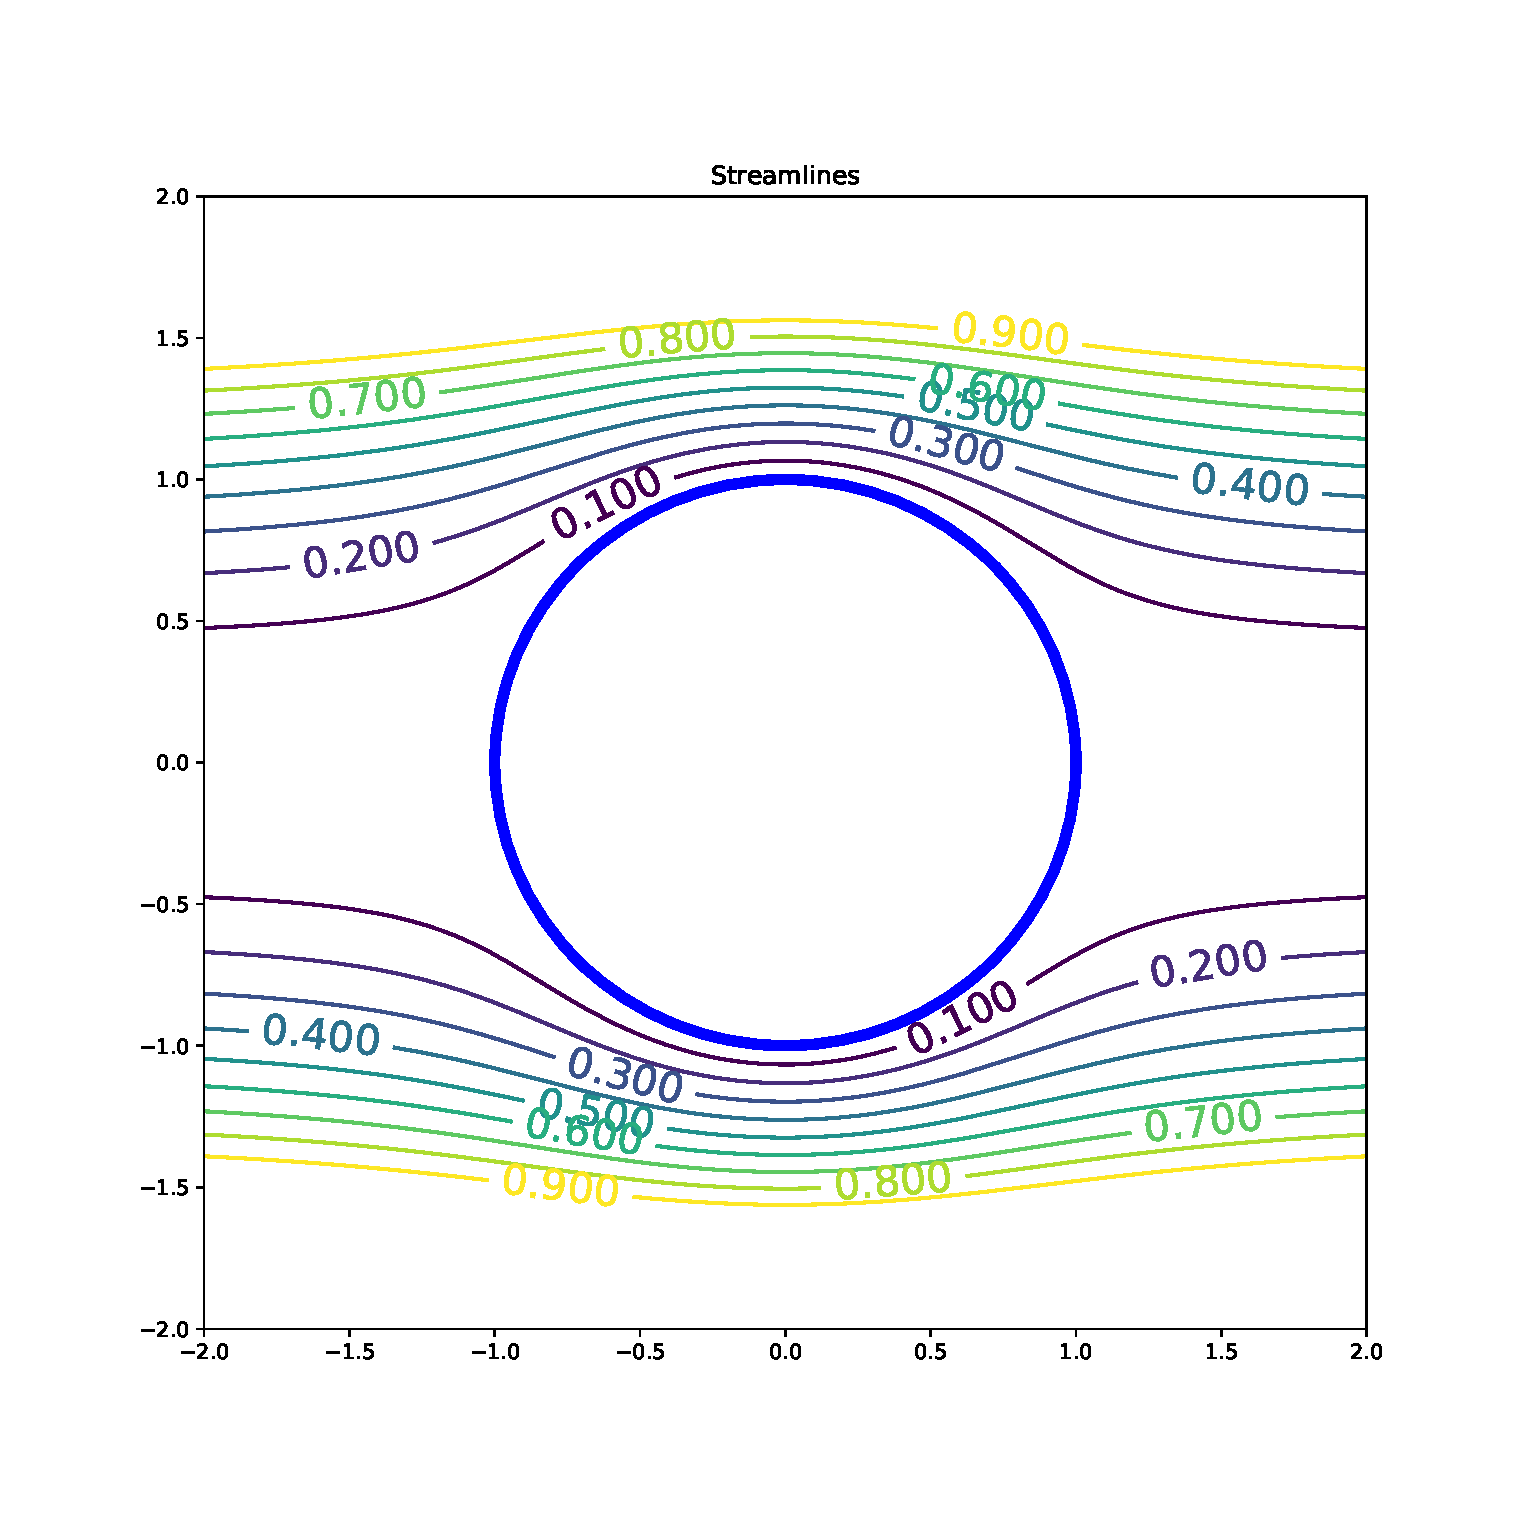
\includegraphics[width=0.4\linewidth]{figures/potential_flow_past_sphere}
  \caption{\label{fig:potential_streamlines_sphere} Streamlines of
    the potential flow past sphere}
\end{figure}



\begin{figure}
  \centering
  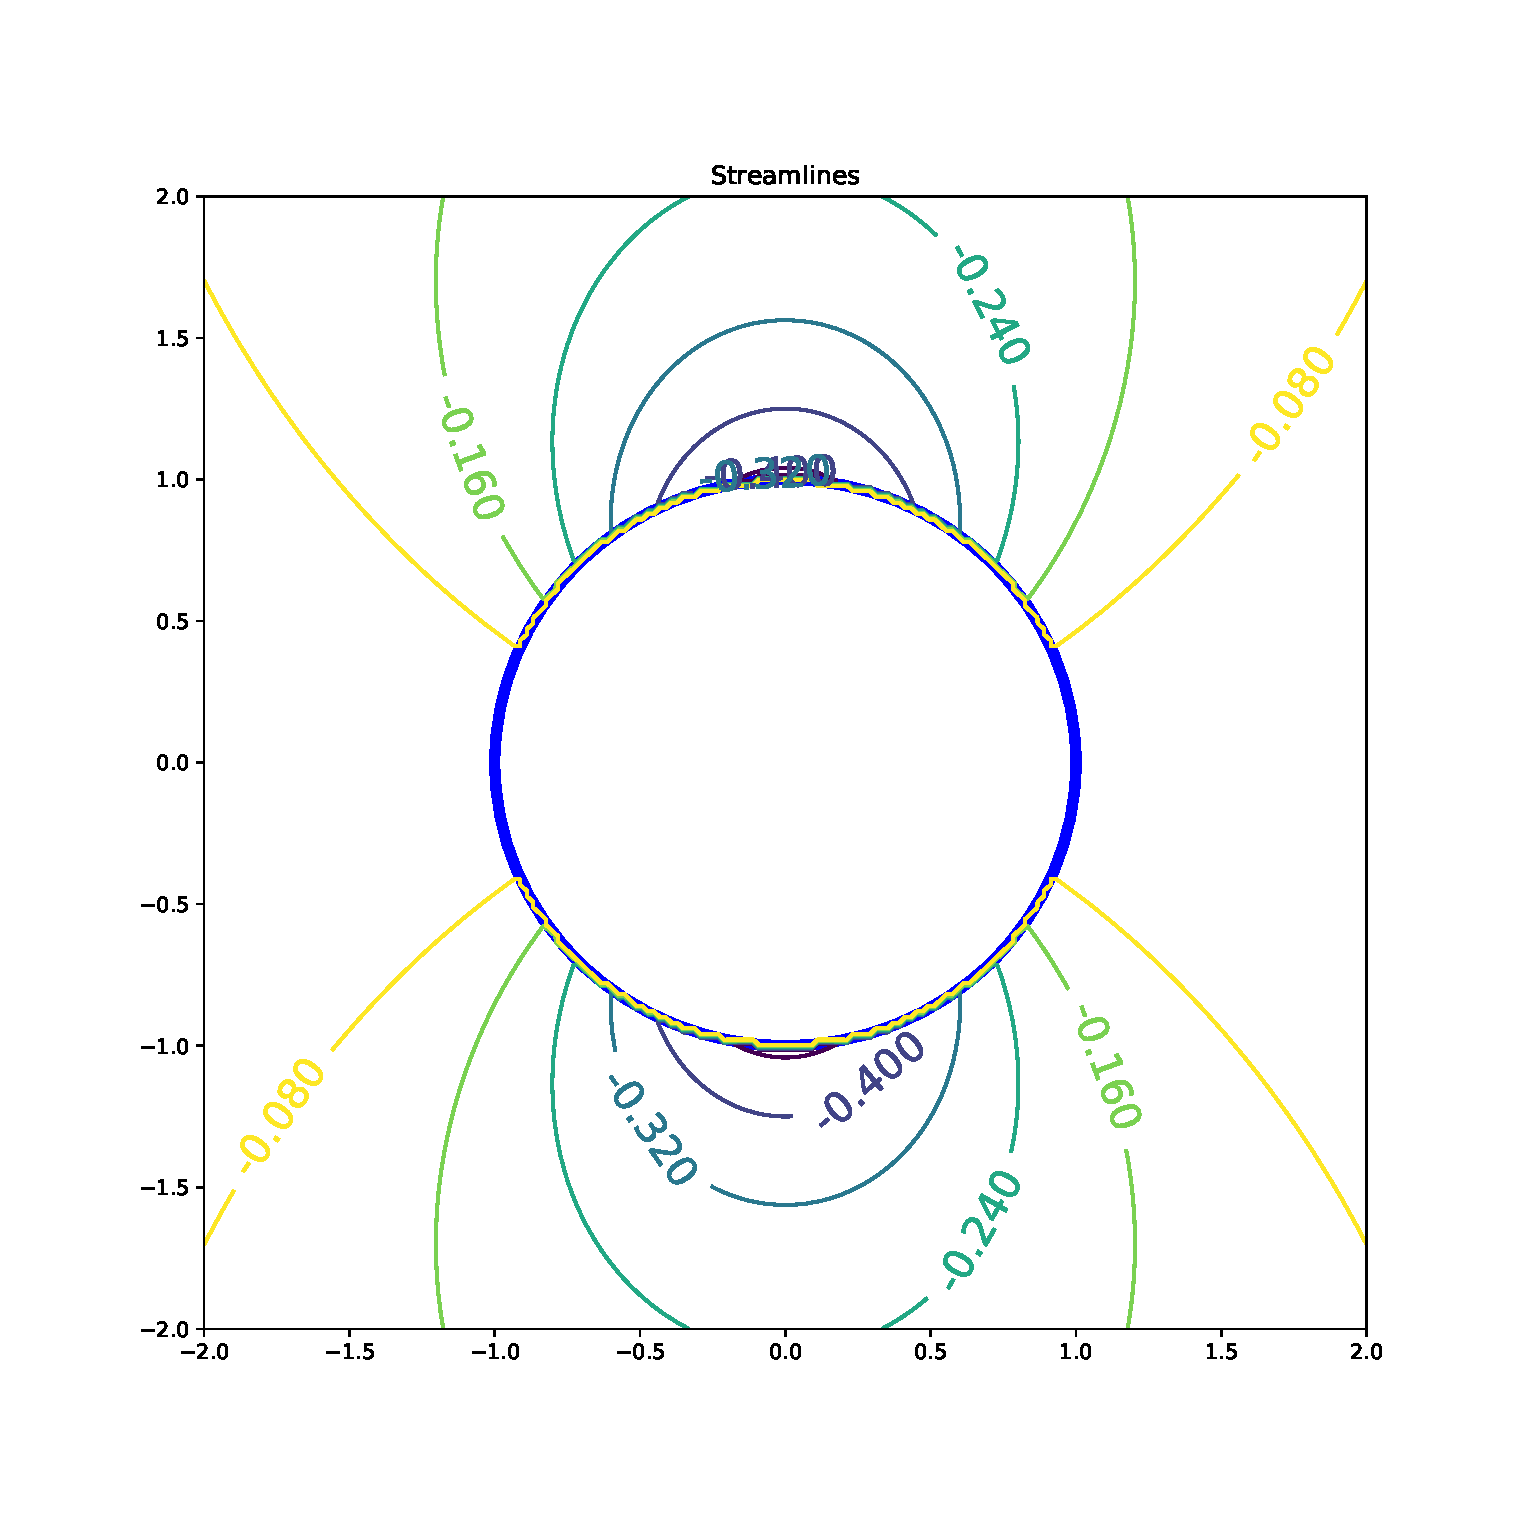
\includegraphics[width=0.4\linewidth]{figures/potential_flow_past_sphere_moving}
  \caption{\label{fig:potential_streamlines_moving_sphere}}
\end{figure}


\subsection{Exercises}

\begin{itemize}
\item \label{ex:u_from_psi_cylinder} 
	The fact that $\nabla\cdot\bfu=0$ implies $\bfu=\nabla\times A$. If
	the flow is, moreover, irrotational, $\nabla\times\bfu = 0$, then
	the vector potential satisfies Laplace's equation, $\nabla^2\bfA=0$,
	given identity \ref{eq:curl_of_curl}. Notice that $\bfA$ is divergence-free
	by construction, since it depends on two spherical coordinates,
	$r$ and $\theta$, while pointing in the other one, $\phi$.
	Solving the Laplace  equation for this field, taking into account the
	appropriate boundary conditions.
%   NO!
%	We have also supposed that
%	$\nabla\cdot\bfA =0$, which in this case is a \emph{choice}, known
%	as ``gauge'' in electromagnetism. Indeed, any addition%
%	$\bfA \to \bfA + \nabla\c$ 

%Derive the velocity field for
%  potential flow around a cylinder from $\psi$, solving the Laplace
%  equation for this field, plus the appropriate boundary conditions.
  
\item \label{ex:u_from_psi_sphere} Derive the velocity field for
  potential flow around a sphere from $\psi$, solving Laplace equation
  for this field with the appropriate boundary conditions. Use the
  the following identity for the Laplacian:
%  
%  fact that Laplace equation $\nabla^2 \bfA = 0$ translates
%  to may be written for
%  $\psi$ using this identity:
  \begin{equation}
    \label{eq:psi_eq_from_A}
    \nabla^2 \left(  \frac{\psi(r,\theta)}{r \sin\theta } \bhe_\phi \right) =
    \frac{1}{r \sin\theta } 
    \left(
      \frac{\partial^2  }{\partial r^2} +
      \frac{1}{r^2} \left[
        \frac{\partial^2 }{\partial \theta^2} - 
        \cot(\theta) \frac{\partial }{\partial \theta}
      \right]
    \right) \psi \bhe_\phi .
  \end{equation}

\item Prove the previous identity. Notice that $\bfA$ is a vector
  field, so one need to apply the expression for the vector Laplacian
  of e.g. \cite{wiki:del}. The expressions are not so bad since the
  field is azimuthal only, and dependent on the other two components:
  $ \bfA = A(r,\theta) \bhe_\phi$.

\item Repeat the previous two calculation using cylindrical
  coordinates. Prove that
  \begin{equation}
    \label{eq:psi_eq_from_A_cyl}
    \nabla^2 \left(  \frac{\psi(\rho ,z) }{\rho} \bhe_\phi \right) =
    \frac{1}{ \rho } 
    \left(
      \frac{\partial^2  }{\partial \rho^2} -
      \frac{1}{ \rho } 
      \frac{\partial  }{\partial \rho} +
      \frac{\partial^2  }{\partial z^2}
    \right) \psi \bhe_\phi .
  \end{equation}
  

\item \label{ex:azimuthal_velocity} Prove that the velocity may
  indeed have an azimuthal component for axisymmetric flow. Begin by
  writing down the expressions for the divergence and the curl in
  spherical coordinates, and neglecting all variation on the azimuthal
  angle, allowing for the possibility that the vector potential may
  have all three components, not just than $A_\phi$.  This result in a
  $u_\phi$ velocity component that can have basically any expression
  as far as continuity is concerned, since it will always be
  satisfied.


\end{itemize}





\chapter{Gravity waves}

\begin{quote}
[Water waves] that are easily seen by everyone and which are usually
used as an example of waves in elementary courses [...] are the worst
possible example [...]; they have all the complications that waves can
have. \hfill (Richard Feynman, \textit{The Feynman Lectures on Physics})
\end{quote}

\section{Gravity waves}

Large waves, like those at the ocean, are driven by gravity. An
initial perturbation on the water surface, like an elevation, will
cause a rise in gravitational potenntial. As this energy is
transferred to kinetic energy, the water around it moves. Similarly to
a pendulum, an area below the mean surface will develop, which will be
filled with surrounding liquid. Thus, the perturbation travels away
from the initial disturbance.

The mathematical treatment of this problem is, in general, very
involved. This is mostly due to the presence of a free surface: the
water-air interface. Mathematically, its location is described by a
height function $\eta$:
\[
z=\eta  \qquad  \eta=\eta(x,y,t) 
\]
(if no overhangs are present). The fluid velocity is to be solved for
a domain between this surface at the ocean bottom, which is supposed
to be flat and at a height $z=-h$ (thus, $z=0$ is taken to be the
surface when no waves occur.)

We have the following boundary conditions for the velocity:
\begin{align}
%  p&=0 \\
  u_z(z=-h) &= 0 \\
  u_z(z=0) &=  \frac{\partial \eta}{\partial t}
\end{align}


The first one is the usual condition at a solid wall, and the last one
is called the ``kinematic condition'', expressing the fact that if the
surface moves up or down, the fluid must do the same in order to be
``stuck to it''.

We will assume an incompressible, irrotational fluid. The fist
assumption is a very reasonable one, and the second one turns out to
be not so bad, since for small waves there is little vorticity
creation (it mainly occurs at the bottom and on breaking waves).  The
assumption of negligible viscosity is likewise not so bad in this
case.



Let us assume a wave train that only depends on the $x$ component
(i.e. waves are very long in the $y$ direction):
\[
\eta = a \cos(kx -\omega t) .
\]
The amplitude $a$, is taken to be small (in the sense $a\ll \lambda$,
and $a\ll h$).

Given the assumptions above, the flow may be treated as a potential
flow, and moreover the only relevant coordinates will be $x$ and
$z$. However, the fields will be time-dependent in this problem,
e.g. $\phi=\phi(x,z,t)$.


The kinematic condition  implies
\[
\left. \frac{\partial \phi}{\partial z}\right|_{z=\eta} =
\frac{\partial \eta}{\partial t} .
\]
This is still a difficult expression, so we will approximate it by
\[
\left. \frac{\partial \phi}{\partial z}\right|_{z=0} =
\frac{\partial \eta}{\partial t} .
\]
(The difference between the two spactial derivatives may be quatified
by a Fourier expansion, in which the neglected terms are seen to be
higher order in $a$).

Let us consider the ansatz
\[
\phi = g(z) \sin(kx -\omega t ) .
\]
The kinematic condition then translates into $g'(0)=a\omega$.

The bottom condition clearly means
\[
\left. \frac{\partial \phi}{\partial z}\right|_{z= -h } = g'(-h)= 0 .
\]


All together, we are looking for a function with these boundary
conditions:
\begin{align}
  g'(0) &=  a \omega \\
  g'(-h) &= 0 .
\end{align}

However, the fact that Laplace equation must be satisfied places a
strong condition on the kind of function $g(z)$ may be:
\[
\nabla^2 \phi = 0 \qquad \implies \qquad
g''(z)  \sin(kx -\omega t ) - g(z)  k^2 \sin(kx -\omega t ) = 0 ,
\]
which meanse
\[
g''(z)  = k^2 g(z) .
\]
Therefore, $g(z)$ must be an exponential function, with the decay
constant being exactly equal to $k$, the wave number. In general, the
solution is a linear combination of two exponentials. Instead of that,
we may write another less conventional expression using hyperbolic
functions. This is equivalent, since these functions are themselves
linear combinaions of exponentials. Moreover, we choose to center them
at $x=-h$ :
\[
g(z)  = a_1 \cosh(k(z+h)) + a_2 \sinh(k(z+h)) .
\]
By inspection, we realize $a_2=0$, since the $\sinh(k(z+h))$ function
was the ``wrong'' behavior at $z=-h$: it has a slope, while the
boundary condition implies it should not.

The kinetic boundary condition implies
\[
a_1 = \frac{a \omega}{ k \sinh(hk)  } .
\]
This is indeed the only value for which $g'(0)= a \omega $. The
potential is then
\[
\phi = \frac{a \omega  \cosh(k(z+h)) }{ k \sinh(hk)  }  \sin(kx -\omega t ) .
\]

From it, the velocity components may be found. These will have a term
featuring $\sin(kx -\omega t )$, a common expression for a traveling
wave. However, the theory is still incomplete since $\omega$ and $k$
are not unrelated in a physical wave, but coupled by the phase
velocity $c=\omega / k$. Remember how in sound waves this velocity was
related to fluid compressibility (to be precise, the square root of
the variation of pressure with density). In this case, such
relationship is as yet missing. Also notice that gravity has played no
role whatsoever, despite claims at the beginning of this chapter about
this factor being the driving force behind this process.

In order to find the missing link, let us remember our previous
expression for the Bernoulli principle, Eq.~\ref{eq:Bern_unsteady},
which can be written as
\[
\frac{\partial \bfu}{\partial t} +
\nabla \cdot \left[
  \frac12 u^2 + \frac{p}{\rho} + \varphi
  \right] =  \frac{p}{\rho}\nabla \cdot \bfu .
\]

In our case the fluid is incompressible, so the right hand side
vanishes. Also, in potential flow we may write the whole equation
compactly:
\[
\nabla \cdot \left[
  \frac{\partial \phi}{\partial t} +
  \frac12 u^2 + \frac{p}{\rho} + \varphi
  \right] =  0 .
\]

This means the whole term on which the divergence operator acts
must be constant in space, but not in time in general:
\[
  \frac{\partial \phi}{\partial t} +
  \frac12 u^2 + \frac{p}{\rho} + \varphi =  f(t) .
\]
This is the less-known unsteady Bernoulli principle.

In this particular case, since boundary conditions do not change in
time (in fact, they do, but we are taking the surface to be close to
$z=0$), any function $f(t)$ may be incorporated into the potential
by making the following trick:
\[
\phi' = \phi + \int_{t_0}^t f(t') dt' ,
\]
hence we may just take $f(t)=0$ in this particular problem.

If we examine the ``head'' term, $ \partial \phi / \partial t +
\frac12 u^2 + \frac{p}{\rho} + \varphi$ at the surface, we notice that
the pressure should be constant (equal to atmospheric pressure, as in
hydrostatics). The $u^2$ may be neglected within our
assumptions. Last, but not least, gravity finally appears in the
potential, $\varphi = g \eta $. This leaves us with
\[
\left.\frac{\partial \phi}{\partial t}\right|_{z=0} + g \eta = 0 ,
\]
often called the ``dynamic condition''. 

With our previous result, this means:
\[
\phi =  - \frac{a \omega^2  \cosh(k(z+h)) }{ k \sinh(hk)  }  \cos(kx -\omega t ) +
g a \cos(kx -\omega t ) =0 .
\]

The result is the following dispersion relation:
\[
\omega^2= g k \tanh(k h)
\]

This is a surprising result, despite being obviously dimensionally
correct, whith the two lengths in the problem, $\lambda=2\pi/k$ and $h$
providing the relevant lenght scales.

We may distinguish two limits.

\subsection{Shallow water}
If the bottom is small, compared to the wavelength $\lambda$, then
$kh = 2\pi h / \lambda $ is a small number, and we may approximate
$\tanh(kh)\approx kh$. Then,
\[
\omega^2= g h  k^2 \qquad \implies \qquad \omega= k \sqrt{g h} .
\]

In this limit, the phase velocity is independent of velocity, which
means the process is non-dispersive:
\[
c =  \frac{\omega}{k} = \sqrt{ g h }  .
\]
The group velocity is of course equal to the phase velocity:
\[
c_\mathrm{g} =\frac{d\omega}{dk} = \sqrt{ g h } = c.
\]

The relevant length in this limit is the depth $h$, which provides the
correct dimensions to get a velocity.

Notice ``shallow'' is defined in relation to the wavelength. A seismic
wave may be excited at the deep sea by a geological process that may
involve tenths or hundreds of kilometers, much larger than the usual
sea depth, which is some few kilometers (its mean value is about
$\SI{3.8}{\kilo\meter}$.) The sea is then ``shallow'', and the speed
at which the perturbation travels will be about
\[
c \approx \sqrt{\SI{9.8}{\meter\per\second\squared} \times
  (\SI{4e3}{\meter}) } \approx \SI{200}{\meter\per\second}
  \approx \SI{700}{\kilo\meter\per\hour} 
\]
This is an astonishing speed, which is nevertheless in agreement with
measurements of these dramatic events.

\subsection{Deep water}

If the bottom is deep, compared to the wavelength $\lambda$, then $kh
= 2\pi h / \lambda $ is a large number, and its hyperbolic tangent is
very nearly $1$. In this limit,
\[
\omega^2 \approx g  k \qquad \implies \qquad \omega= \sqrt{g k} .
\]
These waves are highly dispersive, since their phase velocity depends
on the wavelength:
\[
c =  \frac{\omega}{k} = \sqrt{ g /k  } =  \sqrt{ g \lambda / (2\pi)  }  .
\]

The group velocity is now different from the phase velocity. In fact,
it is one half that value:
\[
2 \log\omega = \log k + \log g \qquad \implies \qquad
\frac{2}{\omega} \frac{d\omega}{dk} = \frac1{k} \qquad  \implies \qquad
c_\mathrm{g} = \frac{c}{2}
\]

In deep waters, the only two length scales we may think of are the
wave amplitude $a$ and their wavength $\lambda$. As we expect the
amplitude to play no role (as long as it is small, $a\ll\lambda$), we
are left with the wavelength to provide the length scale.

Notice that waves high high wavelenghts travel faster. This explains
the groundsell phenomenon, by which waves generated by a far away
storm may arrive quickly at some shore. These waves may precede the
storm by a long time, if the storm does arrive at all. The velocity
grows larger and larger with the wavelength, but as we have seen in
the previous section, as the wavelength becomes comparable to the
depth there will be a crossover to some finite velocity.



\chapter{Work and energy}

Let us find the work done on a fluid particle.

The First Law of thermodynamics tells us this change is due
to work (no heat exchange is considered here):
\[
dE=dW
\]

On the $x$ direction, this work will be given by the distance
travelled by the left wall in the $x$ direction times the pressure
force:
\[
dW_x (\mathrm{left})  = u_x \Delta t p A .
\]

This is work done on the particle (if $u_x$ is positive), hence its
sign. There will be a similar contribution from the right wall, so the
total work given by the $x$ direction will be
\[
dW_x = u_x \Delta t p A  -  u_x'  \Delta t p' A .
\]
By expanding in a Taylor series, this may be written as
\[
dW_x = - \frac{\partial p u_x}{\partial x} \Delta x A \Delta t.
\]

Now, adding the other three components we find
\[
\frac{dW}{dt} = - V \nabla\cdot (p\bfu) .
\]

The right hand side may be expanded
\[
\nabla\cdot (p\bfu) =
 p \nabla\cdot \bfu + 
 \bfu \cdot \nabla p .
\]

Recalling that, from the Euler equation \ref{eq:Euler_momentum} ,
\[
\nabla p  = \rho \bfg - \rho \frac{d \bfu}{dt} ,
\]
we may write
\[
\frac{1}{V} \frac{dW}{dt} =
-  p \nabla\cdot \bfu +
\rho  \bfu \cdot \frac{d \bfu}{dt}  -
\rho  \bfg \cdot  \bfu .
\]

Now, multiplying by $1/\rho$:
\begin{equation}
  \label{eq:specific_energy}
  \frac{d \epsilon }{dt} =
  \bfu \cdot \frac{d \bfu}{dt}  -
  \bfg \cdot  \bfu 
  -  \frac{p}{\rho} \nabla\cdot \bfu ,
\end{equation}
where we have defined the specific energy $\epsilon=E/M$.

This may be written as
\[
\frac{d}{dt} \left[
  \epsilon - \frac12 u^2  + \bfg \cdot \bfr
  \right] = -  \frac{p}{\rho} \nabla\cdot \bfu ,
\]
or
\[
\frac{d}{dt} \left[
  \epsilon - \frac12 u^2  - \varphi
  \right] = -  \frac{p}{\rho} \nabla\cdot \bfu ,
\]
%
This is clearly a law for
\[
e = \epsilon - \frac12 u^2  - \varphi ,
\]
where we define $e$, the specific internal energy as the total energy
minus kinetic energy, minus gravitational potential energy. In other words,
\[
\epsilon  = e  + \frac12 u^2  + \varphi .
\]

The specific internal energy then satisfies a convection equation with
a source term due to the divergence of the velocity
\begin{equation}
  \label{eq:Euler_energy}
  \frac{d e}{dt}  = -  \frac{p}{\rho} \nabla\cdot \bfu ,  
\end{equation}

Notice also that in the steady state,
\[
\bfu \cdot \nabla e = -  \frac{p}{\rho} \nabla\cdot \bfu.
\]
But, recalling our steady Bernoulli principle,
Eq. \ref{eq:Bern_u_times}, replacing
$\frac{p}{\rho} \nabla\cdot \bfu$, we arrive at the steady state
Bernoulli equation for a compressible fluid:
\[
\bfu \cdot \nabla \left[ e + \frac12 u^2 + \frac{p}{\rho} + \varphi
  \right] = 0 ,
\]
%
which tells us the combination $ e + \frac12 u^2 + \frac{p}{\rho} +
\varphi = \epsilon + \frac{p}{\rho} $ is constant along streamlines.
Notice that, by the definition of enthalpy,
\[
H= E + P V ,
\]
the specific enthalpy is
\[
h=H/M = e + p / \rho ,
\]
so the Bernoulli principle claims that the total specific enthalpy
($h'=h + \frac12 u^2 + \varphi$) is constant along streamlines.

We may also find an equation for the enthalpy. In
Eq. \ref{eq:Euler_energy} above, the right hand side may be changed
using the continuity equation:
\[
- \rho \nabla\cdot \bfu = \frac{d\rho}{dt} .
\]
which means
\[
-  \frac{p}{\rho} \nabla\cdot \bfu =
\frac{p}{\rho^2} \frac{d\rho}{dt}
\]

But
\[
\frac{d (p / \rho) }{dt} =
\frac{ 1 }{\rho} 
\frac{d p }{dt} -
\frac{ p }{\rho^2} 
\frac{d \rho }{dt}  .
\]
Hence,
\[
\frac{d ( e + p / \rho) }{dt} = \frac{ 1 }{\rho} \frac{d p }{dt} ,
\]
or
\[
\frac{d h }{dt} = \frac{ 1 }{\rho} \frac{d p }{dt} .
\]
Changes in the enthalpy are therefore tied to changes in pressure.


\subsection{Heat flux}

In the case that some heat flux is present, the First Law of
thermodynamics reads:
\[
dE=dW + dQ .
\]

The influx of heat to the particle, $dQ$, will enter our equations
from a vector heat flux $\bfq$, with units of energy/(area $\times$
time). For example, the heat influx due to transfer in the $x$ direction
will be
\[
dQ_x= \bfq dt dy dz - \bfq(x+dx) dt dy dz \approx
      - V \, dt \, \frac{\partial\bfq}{\partial x},
\]
where in the last approximation a Taylor expansion has been employed,
as should be customary by now.

Altogether, the total heat flux rate is
\[
\frac{dQ}{dt} = -V \nabla\cdot \bfq,
\]
and the final equation for the rate of change of specific internal
energy of an ideal fluid is
\begin{equation}
  \label{eq:Euler_energy_w_q}
  \rho \frac{de}{dt}  = -  p \nabla\cdot \bfu  - \nabla\cdot \bfq .
\end{equation}


The heat flux must be either due to an external source, or due to heat
diffusion. In the latter case, a well-known theory is Fourier's law, by
which the flow is due to a temperature gradient:
\[
\bfq=- k \nabla T ,
\]
where $k$ is the heat diffusion coefficient. The temperature does not
appear in the energy equation, but a common assumption is that
\[
e = c T ,
\]
where $c$ is the specific heat, taken as constant. Then,
\[
\rho  c \frac{d T }{dt}  = - p \nabla\cdot \bfu  + k \nabla^2 T .
\]

For an incompressible fluid,
\[
 \frac{d T }{dt}  = \frac{ k }{ c \rho} \nabla^2 T  = \alpha \nabla^2 T ,
\]
where $\alpha = k / (c \rho)$, a constant if $\rho$ is. This is the
convective Fourier heat equation (it is not the most common Fourier
law, due to the derivative being convective, and not just partial.)




%\chapter{Sample}
%Reference symbols: $\gls{x}$, $\gls{v}$, $\gls{a}$, $\gls{t}$, $\gls{F}$.

\part{Real fluids}


\chapter{Navier-Stokes equations}

\section{Kinematics of a particle}

\label{sec:particle}

Let us focus again on a fluid particle, as we did on Sections
\ref{sec:continuity} and \ref{sec:pressure_forces}, but now focusing
on how the particle itself distorts as a consequence of a velocity
field.

All possible distortions of a particle will be a combination of the
following:
\begin{enumerate}
 \item Translation
 \item Rotation
 \item Shear
 \item Dilation
\end{enumerate}

A translation is just the motion of its center of mass from one place
to another, and for a small time is given simply by $\bfu dt$. The
other motions are more complicated, since they involve spatial
derivatives of the velocity. They must: for a constant velocity field
translation is the only motion that occurs.

\subsubsection{Rotation}

We will refer to particle in figure \ref{fig:}, with vertices A, B,
and C. Vertex D plays no role --- also, it is sufficient to focus on
the face that is portrait, even if the shape of a particle is supposed
to be a cube. It is straightforward to include the other faces, as we
will see.

After a small time $d$ the particle has distorted, so that the
vertices are now at positions A', B', C', and D'.

\begin{figure}
  \centering
  
\includegraphics[width=0.4\linewidth]{figures/particle0}
  \caption{\label{fig:particle0}}
\end{figure}



Let us call $\alpha$ the angle between the $x$ axis and the A'-B'
edge, with the usual counter-clockwise convention as
positive. Similarly, $\beta$ is the angle between the A'-C' edge and
the $y$ axis, with the same convention. It is obvious that a net
rotation takes place if e.g. both angles are positive. If, on the
other hand, they are equal in magnitude but differ in sign, no
rotation takes place. This makes it reasonable to define the
rotation as the average of both angles:
\[
d\Omega_z = \frac12
\left(
        \alpha + \beta
\right) .
\]

Now, angle $\alpha$ will always be very small as $dt$ gets very
tiny. Hence, we may approximate it by its tangent:
\[
\alpha \approx \frac{d\ell}{dx'}
\]



\begin{figure}
  \centering
  
\includegraphics[width=0.4\linewidth]{figures/particle1}
  \caption{\label{fig:particle1}}
\end{figure}

For a small time, we have the following:
\[
dx'=x(B')-x(A') \approx
(dx+v_x(B) dt) - v_x(A) dt \approx
dx+
\left(
v_x(A) +
\frac{\partial v_x}{\partial x} dx
\right ) dt - v_x(A) dt = dx + \frac{\partial v_x}{\partial x} dx dt ,
\]
where we have taken the origin to coincide with the position of A. The
partial derivative is supposed to be evaluated at A, but in the limit
as $dx$ goes to zero it is just ``at the particle''. Similarly, the opposing
side is:
%
\begin{align*}
d\ell & = y(B')-y(A') \approx
y(B) + 
v_y(B) dt
-
y(A) - 
v_y(A) dt \\
& =
\left(
v_y(B) - v_y(A) 
\right) dt 
 \approx
\frac{\partial v_y}{\partial x} dx dt
.
\end{align*}
%
Therefore, to first order in $dt$:
\[
\alpha \approx \frac{\partial v_y}{\partial x}  dt .
\]
In other words, the rate of change of the angle is
\[
\frac{d \alpha}{dt} = \frac{\partial v_y}{\partial x}  .
\]
Notice the cross derivative: what is relevant is the change of the
vertical component of the velocity with the horizontal coordinate.

A similar calculation for the other angle reveals
\[
\frac{d \beta}{dt} = - \frac{\partial v_x}{\partial y}  .
\]

Taking all
\[
\frac{d\Omega_z}{dt} = \frac12
\left(
  \frac{\partial v_y}{\partial x}  -
  \frac{\partial v_x}{\partial y}
\right) .
\]

This may sound familiar to the reader, since the curl in Cartesian
coordinates has a $z$ component with exactly the same expression, but
the factor of $1/2$. This analysis may be carried out for
rotations about the other two Cartesian axes, with the end result that
\[
 \frac{d \bm{\Omega} }{dt} = \frac12 \vort .
\]

The curl is therefore twice the rate of rotation of a fluid particle.


As an example, let us consider a uniform circular motion about the
origin:
\[
\bfr =
\begin{cases}
x =r \cos(\omega_0 t) \\
y =r \sin(\omega_0 t) .
\end{cases}
\]
The velocity field is
\[
\bfu =
\begin{cases}
u_x= -r \omega_0 \sin(\omega_0 t) = -\omega_0 y \\
u_y=  r \omega_0 \cos(\omega_0 t) =  \omega_0 x.
\end{cases}
\]

If we compute the curl of this field, its only component is the $z$ one:
\[
\omega_z= \left(
  \frac{\partial (\omega_0  x)}{\partial x}  -
  \frac{\partial (- \omega_0 y) }{\partial y}
\right) =  2 \omega_0 . 
\]

Therefore, the curl indeed is twice the angular velocity.

Finally, let us recall, from the definition of the tensor
$\nabla \bfu$ of Eq. \ref{eq:nabla_u_def},
\begin{equation}
  \label{eq:dOmega_as_grad_u}
  \frac{d\Omega_{ij}}{dt} = \frac12
  \left[
    (\nabla \bfu)_{ij} -
    (\nabla \bfu)_{ji}
  \right] ,  
\end{equation}
%
where the cyclic convention $(i,j,k)$ is implied in order to relate
the indices of $d\Omega_{ij}/ dt$ and the components $d\Omega_k/ dt$
(see Exercise \ref{ex:dOmega_LC} for a definition in terms of the
Levi-Civita symbol.)


\subsubsection{Strain}

Similarly to the definition of rotation, let us define the strain as
half the difference between angle $\beta$ and $\alpha$:
\[
d\epsilon_{xy} = \frac12
\left(
        \alpha - \beta
\right) .
\]
Indeed, if both are equal we get a pure rotation, and no strain. If,
however, they have the same magnitude but opposite sign, we have a pure
strain and no rotation.

This definition leads to
\[
\epsilon_{xy} = \frac12
\left(
  \frac{\partial v_y}{\partial x}  +
  \frac{\partial v_x}{\partial y}
\right) .
\]

Notice the notation: indices $xy$ implay a strain on that plane. In general,
\[
\epsilon_{ij} = \frac12
\left(
  \frac{\partial v_j}{\partial x_i}  +
  \frac{\partial v_i}{\partial x_j}
\right) .
\]

This defines off-diagonal terms of a tensor that is obviously
symmetric. All together, three terms in 3D ($xy$, $xz$, and $yz$).

Also, from the definition of the tensor $\nabla \bfu$ of
Eq. \ref{eq:nabla_u_def},
\begin{equation}
  \label{eq:epsilon_as_grad_u}
  \epsilon_{ij} = \frac12
  \left[
    (\nabla \bfu)_{ij} +
    (\nabla \bfu)_{ji}
  \right] ,
\end{equation}
so that $\epsilon$ is the symmetrized version of the gradient of the
velocity.

We may also extend these definitions to the diagonal terms:
\[
  \epsilon_{ii} =   \frac{\partial v_i}{\partial x_i} ,
\]
which are not really strains, as we show next.

\subsubsection{Dilation}

We have derived before that the change on side $dx$ is
\[
dx' \approx  dx + \frac{\partial v_x}{\partial x} dx dt ,
\]
which features the diagonal components of the strain tensor just
introduced. In general, for the $i$ Cartesian direction,
\[
dx_i' \approx dx_i + \epsilon_{ii} dx_i dt = dx_i
\left(
1+\epsilon_{ii} dt
\right)
\]

If we consider the volume, its new value will be
\[
V'= dx' dy' dz'  \approx  \prod_i  dx_i \left( 1+\epsilon_{ii} dt \right)
\approx \left(\prod_i  dx_i \right) \left( 1 + \sum_j  \epsilon_{jj} dt \right) ,
\]
where in the last expression we have neglected all higher order terms
($dt^2$ or higher). Therefore, the new volume of a particle is
\[
V' = V \left( 1 + \sum_j  \epsilon_{jj} dt \right) .
\]
Its change is
\[
V'-V =  V \sum_j  \epsilon_{jj} dt .
\]
In the limit as $dt\to 0$,
\[
\frac{d V}{dt} = V \sum_j  \epsilon_{jj} .
\]
This clearly identifies the diagonal components of the strain tensor
as those responsible for the relative rate of change of the volume.
Moreover, due to its definition, the sum of all components (i.e. the
trace of the tensor) is precisely the divergence of the velocity:
\[
\sum_j  \epsilon_{jj} = \nabla\cdot \bfu .
\]

We therefore arrive at the expression for the rate of change of a particle:
\[
\frac{d V}{dt} = V  \nabla\cdot \bfu .
\]

\subsection{Continuity, re-revisited}
\label{sec:continuity3}

This is the expression that was lacking in our derivation in
Section \ref{sec:continuity}. Indeed, if the mass of a particle is
constant, it is trivial to recover the continuity equation for the
density. The latter is $\rho=m/V$, therefore,
\[
\frac{d \rho }{dt} =
\frac{d (m/V) }{dt} = \frac1V \underbrace{\frac{ dm }{dt}}_{=0} -
m\frac1{V^2}  \frac{ dV }{dt } =
- m\frac1{V}  \nabla\cdot \bfu  = -\rho \nabla\cdot \bfu ,
\]
which indeed is the right expression (the ``convergence'' Equation
\ref{eq:convergence}.)

This also shows that we are working on an Lagrangian reference frame, so
that advective derivatives appear naturally. Indeed, $dm/dt=0$ for a
particle, whereas mass may enter and leave a fixed (Eulerian) zone in
space.



\section{Stress tensor}

Let us return again to our particle in order to analyze its movement
when stress forces are applied onto its walls. The pressure force may
be consider a special case of the latter, but stress forces may also
have a shear component.

Thus, the horizontal force will be given by, in part, by the
contributions due to the walls at the left, back, and bottom
\begin{equation}
  \label{eq:wall_shear_stress}
  \left. dF_x \right|_\text{l,bk,bm} =
  % - p         dy\, dz
    \tau_{xx} dy\, dz +
    \tau_{yx} dx\, dz +
    \tau_{zx} dx\, dy .
\end{equation}
%
The compression stress $\tau_{xx}$ is therefore quite similar to the
pressure (see (Eq  \ref{eq:pressure_force_on_left}), and in fact
will be seen to include a $-p$ term. The minus sign appears because
normal stresses are historically defined as positive if pointing
outside the particle (i.e. in the direction of the normal vector).
%
%where we include not only the pressure force, as before 
%and a compression stress $\tau_{xx}$ quite similar to it,
In addittion, two shear stress forces appear. One of them, $\tau_{yx}
dx\, dz$ is the horizontal shear force on the back wall ($dx\, dz$
actually equals $dx\, dy$, but it is clearer to write it this
way). Similarly, $\tau_{zx} dx\, dy $ is the horizontal stress force
at the bottom wall.

Notice the convention for labeling: $\tau_{ij}$ is the stress in the
$j$ direction on a face normal to axis $i$. I.e. the left face has the
same convention as the right one, the back as the front, the top as
the bottom.

%First, the normal stress is
%$\tau_{xx} \parallel \bfn $. From it,
%$\tau_{xy} \parallel \bfe_z\times \tau_{xx} $,
%$\tau_{xz} \parallel \tau_{xx} \times \bfe_y $, respecting the
%$(x,y,z)$ cyclic order. A quick way to realize this is by considering
%the top face, on which these three directions coincide with the
%Cartesian axes. The directions on other faces are found by rotating
%these directions accordingly. The right hand may be used for this
%purpose.

To get the whole horizontal force, the contributions from the other
three walls must be considered:
\[
\left. dF_x \right|_\text{r,ft,up} =
%- p         dy\, dz
  \tau_{xx}(x+dx,y   ,z   )  dy\, dz +
  \tau_{yx}(x   ,y+dy,z   )  dx\, dz +
  \tau_{zx}(x   ,y   ,z+dz)  dx\, dy .
\]
%This time, the sign convention is positive.

To get the total horizontal force due to stresses, the two contributions
must be subtracted:
\begin{align*}
dF_x = 
&\left( \tau_{xx}(x+dx,y   ,z   ) - \tau_{xx} \right) dy\, dz + \\
&\left( \tau_{yx}(x   ,y+dy,z   ) - \tau_{yx} \right)  dx\, dz + \\
&\left( \tau_{zx}(x   ,y   ,z +dz  ) - \tau_{zx} \right) dx\, dy 
\end{align*}.
Notice that the substraction is in order: if the stresses are the same
on those faces, the resultant force will then be zero (those forces
may exert a net torque, but not a force).  In general, they will be
different on those faces, as as been made explitic on their arguments.

The choice is such that an variation in a given direction is assigned
a positive sign. This affects later results, in particular the fact
that the pressure appears with a negative sign.

Expanding in Taylor series, we get the following net horizontal force:
\[
 dF_x  =
%-\frac{\partial p      }{\partial x}  dx\, dy\, dz
% +
 \left(\frac{\partial\tau_{xx}}{\partial x}  dx\right)\, dy\, dz
+\left(\frac{\partial\tau_{yx}}{\partial y}  dy\right)\, dx\, dz
+\left(\frac{\partial\tau_{zx}}{\partial z}  dz\right)\, dx\, dy .
\]

The volumetric horizontal force is then,
\[
f_x  =
%-\frac{\partial p      }{\partial x}
 %+
 \frac{\partial\tau_{xx}}{\partial x}
+\frac{\partial\tau_{yx}}{\partial y}
+\frac{\partial\tau_{zx}}{\partial z} .
\]

With integer notation for Cartesian coordinates:
\[
 f_1  =
%-\frac{\partial p      }{\partial x_1}
 %+
 \sum_{j=1,2,3}
 \frac{\partial\tau_{j1}}{\partial x_j} .
\]


In general, for any component we will have:
\[
 f_i  =
%-\frac{\partial p      }{\partial x_i}
 %+
 \sum_{j=1,2,3}
  \frac{\partial\tau_{ji}}{\partial x_j} .
\]

In order to use vector notation, we have to introduce the
divergence of a tensor:
\[
\nabla \cdot \tau = \sum_{j=1,2,3}
  \frac{\partial}{\partial x_j}  \tau_{ji} ,
\]
 which results in a vector:
\[
 \bff  =
%-\nabla p
 %+
 \nabla \cdot \tau .
\]
%
The tensor $\tau$ has components $\tau_{ij}$. There is also
the matrix notation, by which
\[
\nabla \cdot \tau = \nabla\tran  \tau ,
\]
where $\nabla\tran$ is a transposed (row) vector operator, multiplying
matrix $\tau$ from the left.

The resulting Navier-Stokes momentum equation is then
\begin{equation}
  \label{eq:NS}
  \rho \frac{d\bfu }{dt} = \nabla \cdot \tau   + \rho \bfg .
\end{equation}



\subsection{Newtonian fluids}
\label{sec:Newtonian}

The previous equation is still too general, and a connection between
stress and strain is still needed. Here we consider the case in which
there is a linear relationship between both, which involves the
coefficient of viscosity.

To begin with, let us consider a simple case in which a fluid is
confined between two planes. One of them moves sideways with a certain
speed $u_0$, while the other is kept fixed. After a certain transient,
some force is needed in order to keep this shearing. The simplest
expression is
\begin{equation}\label{eq:Newton_simple_law}
F= \mu A \frac{u_0}{L} .
\end{equation}
The force is proportional to the area and to the velocity difference
between the planes. It is also inversely proportional to their
separation, $L$ (this fact being the least obvious). Finally, a
constant of proportionality is given by $\mu$, the viscosity
coefficient, or simply ``the viscosity''. This constant may vary with
temperature, density, pressure, but the point with Newtonian fluids is
that it does not vary with the velocity field (or its
derivatives). Later, in section \ref{sec:Couette}, this flow will be
solved as a solution of the Navier-Stokes equations, the Couette
flow. There, it will be shown that the velocity is everywhere in the
direction of the force exerted on the upper plane, let us call it $x$,
and varies linearly between the planes, in the $y$
direction. Therefore, the only components of the strain rate tensor
are $\epsilon_{xy} = \epsilon_{yx} = u_0 / ( 2 L )$. We therefore have
\[
\tau_{xy} = \mu  \epsilon_{xy} .
\]

With these in mind, let us look for a general relationship between
$\tau$ and $\epsilon$. This is much easier if we go to the principal
strain axes. These are the coordinates on which the strain rate is
diagonal. Such coordinate system always exist, since the strain rate
tensor is symmetric. Notice that in these system strains are not due to
shear, only to dilations.

A simple example would be to consider the flow $u_x = u_0 y / L$
(again, Couette flow). In this case,
\[
\epsilon=
\begin{pmatrix}
  0           &   u_0/(2L)  \\
   u_0/(2L)   &   0
\end{pmatrix} .
\]

It is easy to find the two eigenvalues and associated eigenvectors of
this matrix:
\begin{align*}
  \lambda_1=  u_0/(2L) \qquad &\bfv_1=(1/\sqrt{2}) \begin{pmatrix} 1 &  1 \end{pmatrix}\tran \\
  \lambda_2= -u_0/(2L) \qquad &\bfv_2=(1/\sqrt{2})  \begin{pmatrix} 1 &  -1 \end{pmatrix}\tran \\
\end{align*}
Notice the first eigenvalue correnspond to a dilation along the $x=y$
diagonal, while the second is a compression along the $x=-y$ one.

The diagonal strain rate matrix is then:
\[
\tilde{\epsilon}=
\begin{pmatrix}
  u_0/(2L)   & 0 \\
  0          & - u_0/(2L)
\end{pmatrix} .
\]

It is crucial to realize that the stress tensor is also diagonal in
this coordinate system. Otherwise, a pure dilation in one of the
principal directions would cause a shear stress in some other
direction. This does not mean, however, that the two tensors are
simply proportional. Instead, we may posit, for the top-most element
\[
\tilde{\tau}_{xx}=
- p + 
C_1 \tilde{\epsilon}_{xx} +
C_2 \tilde{\epsilon}_{yy} +
C_3 \tilde{\epsilon}_{y} .
\]
We have added a $-p$ term that has to be there even when there is no
movement. This is needed, since a diagonal stress tensor $\tau=-p\eye$
produces the $-\nabla p$ term of hydrostatics (in Couette flow, $p$ is
constant, and this term is not needed.) The minus sign of $-p$ stems
from the fact that the pressure force points toward the interior of a
particle.

If isotropy is assumed, there should be no distinction between
traverse directions $y$ and $z$. Therefore, $C_2=C_3$, and
\[
\tilde{\tau}_{xx}=
- p + 
C_1 \tilde{\epsilon}_{xx} +
C_2 ( \tilde{\epsilon}_{yy} +  \tilde{\epsilon}_{y}  ) =
- p + 
K \tilde{\epsilon}_{xx} +
C_2 ( \tilde{\epsilon}_{xx} + \tilde{\epsilon}_{yy} +  \tilde{\epsilon}_{y}  ) ,
\]
where the constant $K=C_1-C_2$. Notice the $C_2$ term is the
divergence of the velocity. But, it is also the trace of the strain
tensor, a quantity which is invariant under change of basis. We can
now write:
\[
\tilde{\tau}_{xx}=
- p + C_2 \nabla\cdot \bfu +
K \tilde{\epsilon}_{xx} .
\]

There will be similar expressions for $\tilde{\tau}_{yy}$ and
$\tilde{\tau}_{zz}$, but in them the coefficients must be the same ---
otherwise isotropy will be violated. Taking all together,
\[
\tilde{\tau}=
K \tilde{\epsilon}
+ ( - p + C_2 \nabla\cdot \bfu ) \eye.
\]

Now, we may go back to the original Cartesian system and find
\[
\tau=
K \epsilon
+ ( - p + C_2 \nabla\cdot \bfu ) \eye.
\]
The stress tensor is then also symmetric, a fact that is required in
order the particle be torsion-free (remember the fact that rotations
have no stress associated.)

A comparison with our previous result reveals $K=2\mu$. The constant
$C_2$ is called, in the theory of elasticity ``the second Lam\'e
coefficient'', and receives the symbol $\lambda$ (it is also called
the ``second viscosity coefficient'', $\mu$ being the first.) Then,
\[
\tau=
2 \mu \epsilon + ( - p + \lambda \nabla\cdot \bfu ) \eye.
\]

To make this explicit, this means that diagonal terms have the form
\begin{equation}
  \label{eq:tau_diagonal}
  \tau_{ii}=
  2 \mu \epsilon_{ii}  - p + \lambda \nabla\cdot \bfu ,
\end{equation}
while off-diagonal terms are
\begin{equation}
  \label{eq:tau_off_diagonal}
  \tau_{ij}=  2 \mu \epsilon_{ij} \qquad j \ne i
\end{equation}


(Why not always work in the system of principal axes? The answer is
simple: principal axes vary from one particle to another, since they
are defined by local values of velocity derivatives. The Cartesian
coordinate system, or any such (cylindrical, polar\ldots) is the same
for all particles.)

The off-diagonal terms have a neat expression when the strain rate
tensor is written in term of velocity derivatives:
\[
\tau_{ij}=
\mu
\left(
\frac{\partial u_i}{\partial x_j} +
\frac{\partial u_j}{\partial x_i}
\right)
\]

The diagonal ones, however, are somewhat puzzling:
\[
\tau_{ii}=
- p +
2 \mu \frac{\partial u_i}{\partial x_i}  + \lambda \nabla\cdot \bfu .
\]
The pressure term is natural, but there are two extra dynamical terms.

Let us define a mechanical pressure as minus one-third times the trace
of the stress tensor:
\[
\bar{p}=
-\frac13 \Tr \tau  = 
 p
- \left( \frac23 \mu  + \lambda \right) \nabla\cdot \bfu .
\]

Defining volume viscosity as
\begin{equation}
  \label{eq:vol_visc_definition}
  \eta:=\frac23 \mu  + \lambda,
\end{equation}
we may write the mechanical pressure as
\begin{equation}
  \label{eq:mech_p_definition}
  \bar{p} :=
  p - \eta \nabla\cdot \bfu .
\end{equation}
%
The result is that the mechanical pressure, defined this a way, is
\emph{different} from the thermodynamic pressure in an incompressible
fluid.  There are several ways out of this puzzling result. One of
them is to assume simply that the fluid is incompressible. This is of
course entirely correct, but would limit the applicability of the
theory to incompressible problems.

Another approach is to boldly assume $( 2/3 ) \mu+\lambda=0$. This
step was taken by Stokes, and defines a ``Stokesian fluid''. On the
other hand, there is no clear evidence of a real fluid that may
satisfy such a relationship. Indeed, the few measures of $\lambda$
have show positive values (while $\mu$, as should be clear, is always
positive). We should then keep in mind that in some flows when
compressibility is important, mechanical pressure may differ from
thermodynamical one. One such example is the attenuation of sound
waves, explained in Section \ref{sec:sound_waves_att}.

The Navier-Stokes equation for Newtonian liquids is finally:
\begin{equation}
  \label{eq:NS_Newtonian}
  \rho \frac{d\bfu }{dt} =
  - \nabla p +
  2 \nabla \cdot ( \mu \epsilon)
  + \nabla [ \lambda ( \divu ) ]
  + \rho \bfg .
\end{equation}



\subsubsection{Pure shear and compression}

Recalling the definition of the strain tensor $\epsilon$
in Eq. \ref{eq:epsilon_as_grad_u}, the viscous force may be written as
\begin{equation*}
  \bff_\mathrm{v}=
  \nabla \cdot \left[ \mu  \left( \nabla\bfu + \nabla\bfu\tran \right) \right] +
  \nabla \cdot \left[ \lambda (\divu) \eye \right] ,
\end{equation*}
where $\nabla \cdot \left[ A \eye \right] $ is just another way to
write $\nabla A$, for any scalar field $A$.


If the volume viscosity of Eq. \ref{eq:vol_visc_definition} is
introduced, the equation may be rearranged to read
\begin{equation}
  \label{eq:pure_stress_pure_compression}
  \bff_\mathrm{v}=
  \nabla \cdot \left[ \mu  \left(
      \nabla\bfu + \nabla\bfu\tran  - \frac23 (\divu)  \eye
    \right)
  \right] +
  \nabla \cdot \left[ \eta (\divu) \eye \right] .
\end{equation}
This expression is rather elegant, since the term multiplied by $\mu$
describes pure shear flow, with no compression effects, and the term
with $\eta$, pure compression.

This is easily demonstrated, since
\[
  \Tr  \nabla\bfu = \divu \qquad\implies\qquad \Tr \left( \nabla\bfu -\frac13 (\divu) \eye \right) = 0 .
\]
The same goes for $ \nabla\bfu\tran$, hence the $2/3$ factor.


\subsection{Particular instances}

We here consider instancies in which Eq. \ref{eq:NS_Newtonian} for
Newtonian liquid is further simplified.


\subsubsection{Athermal case}

It may happen that the viscosity coefficients do not vary, when the
variations on the other fields are not too great. In particular,
viscosity depends on temperature quite strongly, as is evident when
heating up oil. The temperature has its own equation, to be explained
in the next chapter. In this case, Eq. \ref{eq:NS_Newtonian} may be
written as
\begin{equation*}
  \rho \frac{d\bfu }{dt} =
  - \nabla p +
   2 \mu \nabla \cdot  \epsilon
  + \lambda \nabla ( \divu ) )
  + \rho \bfg .
\end{equation*}

Now, $\nabla \cdot  \nabla\bfu = \nabla^2 \bfu$, as can be demonstrated
since the $i$-th component of the resulting vector is
\[
(\nabla \cdot \nabla\bfu )_i =
\sum_{j=1,2,3} 
\frac{\partial}{\partial x_j} 
\frac{\partial u_i}{\partial x_j}
=
\sum_{j=1,2,3} 
\frac{\partial^2 }{\partial x_j^2} 
u_i = \nabla^2 u_i .
\]

However, $\nabla \cdot  \nabla\bfu\tran = \nabla  (\divu)$:
\[
(\nabla \cdot \nabla\bfu\tran )_i =
\sum_{j=1,2,3} 
\frac{\partial}{\partial x_j} 
\frac{\partial u_j}{\partial x_i}
=
\frac{\partial}{\partial x_i} 
\sum_{j=1,2,3} 
\frac{\partial u_j }{\partial x_j} 
= (\nabla  (\divu))_i .
\]

This means the NS equation can be written, in this limit,
as
\begin{equation}
  \label{eq:NS_const_viscs}
  \rho \frac{d\bfu }{dt} =
  - \nabla p +
   \mu \nabla^2  \bfu
  + ( \lambda  + \mu) \nabla ( \divu ) )
  + \rho \bfg .
\end{equation}



If the mechanical pressure (\ref{eq:mech_p_definition}) is used instead,
\begin{equation}
  \label{eq:NS_const_viscs_mech_press}
  \rho \frac{d\bfu }{dt} =
  - \nabla \bar{p} +
  \mu \nabla^2  \bfu
  + \frac13  \mu \nabla ( \divu ) )
  + \rho \bfg ,
\end{equation}
where one the shear viscosity appears (the other one being swept under
the rug, in the mechanical pressure.)


\subsubsection{Incompressible, athermal case}

If, in addition to having constant viscosity coefficients, the flow is
incompressible, the terms with $\divu$ in the previous section may be
neglected.

The final momentum equation for an incompressible, athermal fluid, is
then
\begin{equation}
  \label{eq:NS_usual}
  \rho \frac{d\bfu }{dt} =
  - \nabla p 
  + \mu \nabla^2 \bfu
  + \rho \bfg .
\end{equation}
This equation, in this particular form, is the beginning of a vast
ammount of research in physics and applied mathematics.





\section{Dimensionless variables: the Reynolds number}

For the simplest, athermal incompressible case, the term due to
viscosity
\[
\mu \nabla^2 \bfu = \mu \frac{u_0}{L^2} \nabla^{*2} \bfu^* ,
\]
where we cast the variables into reduced form, as explained in
section \ref{sec:Euler_adim}.

Recall that in order to arrive to \ref{eq:Euler_just_before_adim}, the
whole equation was multipled by $L/(\rho_0 u_0^2)$. If we do that to our
momentum equation, the result is
\[
\rho^* \frac{d\bfu^* }{dt^* } =
-  \nabla^* p^*
+  \rho^* \bfg^* +
\frac{\mu }{\rho_ 0 L u_0 } \nabla^{*2} \bfu^* .
\]

The term $\mu /( \rho_ 0 L u_0)$ must be dimensionless (as can be
easily checked). It then represents a reduced viscosity, and should be
taken as such: a number that defines whether viscosity is important or
not in a given context.

Historically, however, it is its inverse that has a name, the
Reynolds' number:
\begin{equation}
  \mathbf{Re}= \frac{\rho_ 0 L u_0 }{\mu }.
\end{equation}

This number is therefore large when viscosity is small, and small when
it is large. It may also be defined as the ratio of inertial forces and
viscous forces:
\begin{equation}
  \mathbf{Re}= \frac{\rho_ 0 u^2_0 }{\mu u_0 / L }.
\end{equation}
Indeed, in the numerator $\rho_ 0 u^2_0$ is the typical strength of the
pressure, and in the denominator $\mu u_0 / L $ is the typical
strength of viscous stress forces.

In many mathematical contexts, all dimensions are forfeited, and the
momentum equation is simply written as
\begin{equation}
  \label{eq:NS_usual_reduced}
  \frac{d\bfu }{dt} =
  - \nabla p 
  + \frac{1}{\mathbf{Re}} \nabla^2 \bfu
  + \bfg .
\end{equation}







\section{Vorticity}
\label{sec:NS_vort}

Let us begin applyy the method in Sec. \ref{sec:NS_vort} to our
momentum equation for a Newtonian fluid undergoing athermal
incompressible flow,\ref{eq:NS_usual}, in order to obtain an equation
for the vorticity and velocity alone.
\begin{equation*}
  \frac{\partial \bfu }{\partial t}
  + \bfu \nabla \bfu
  =
  - \nabla p 
  + \nu \nabla^2 \bfu
  + \bfg ,
\end{equation*}
(where ``$p$'' is actually ``$p/\rho$'', as customary in
incompressible flow), we may begin modifying the convective
acceleration using Lamb's identity \ref{eq:Lambs_identity}:
\begin{equation*}
  \frac{\partial \bfu }{\partial t}
  + \frac12 \nabla (u^2)
  -\bfu\times\vort
  =
  - \nabla p 
  + \nu \nabla^2 \bfu
  + \bfg .
\end{equation*}
The viscous term may be written as
$\nabla^2 \bfu = -\nabla\times\vort$, from the expression for the curl
of a curl \ref{eq:curl_of_curl} for incompressible flows. Taking the
curl of this expression, all the terms that are gradients of fields
vanish, and we get
\begin{equation*}
  \frac{\partial \vort }{\partial t}
  -\nabla\times (\bfu \times \vort )
  =
  -\nu  \nabla\times\nabla\times\vort .
\end{equation*}
Now, the curl of a vector product may be simplified as in Section
\ref{sec:Euler_vorticity}, $\nabla\times (\bfu \times \vort ) =
-\bfu\nabla\vort + \vort\nabla\bfu$ (again, valid for incompressible
flow). The double curl can again be cast as minus the Laplacian, since
the curl is always divergence-free.

Therefore,
\begin{equation*}
  \frac{\partial \vort }{\partial t} +
  \bfu\nabla\vort 
  =
  \vort\nabla\bfu
  +\nu  \nabla^2\vort .
\end{equation*}

Finally,
\begin{equation*}
  \frac{d \vort }{d t}
  =
  \vort\nabla\bfu
  +\nu  \nabla^2\vort .
\end{equation*}

This is clearly the Euler expression for the evolution of vorticity,
times an extra, diffusion term. The constant of diffusivity is $\nu$,
the same as velocity. It may seem that little is changed from that
situation. The reality is much different: it is actually the boundary
conditions which are usually sources of vorticity, which is then
carried onto the rest of the fluid by a combination of advecion and
diffusion. The ratio of these two processes depend of course on the
particular fluid (through $\nu$) and the flow features.


\section{Exercises}

\begin{enumerate}
\item \label{ex:dOmega_LC}
  Cast Eq. \ref{eq:dOmega_as_grad_u} as
  \[
    \frac{d\Omega_{k}}{dt} = \frac12 \epsilon_{ijk}
    \left[
      (\nabla \bfu)_{ij} -
      (\nabla \bfu)_{ji}
    \right] ,
  \]
  where summation over repeated indices is implicit (Einstein's
  convention) \index{Einstein's convention}, and $\epsilon$ is the
  Levi-Civita symbol, see Exercise \ref{ex:vector_identity} of Section
  \ref{sec:Euler_exercises}.

\item Check that $\mu /( \rho_ 0 L u_0)$ is indeed dimensionless.
\end{enumerate}





\chapter{The energy equation}
In addition to continuity and momentum, there is an additional
Navier-Stokes equation for the energy.

It contains the previous expression for ideal fluid, plus a term
expressing energy dissipation by viscosity.

We must re-evaluate the work done on each of the faces of the
particles due to stresses. For example, on the left wall the energy
due to stress forces is
\[
dW(\mathrm{left})  =
 -(u_x dt)   \tau_{xx} dy dz
 -(u_y dt)   \tau_{xy} dy dz
 -(u_z dt)   \tau_{xz} dy dz .
\]

Each of the stresses on this wall does work only in its direction of
motion: $\tau_{xx}$ is compression and will feature a $-p$ term, which
$\tau_{xy}$ and $\tau_{xz}$ produce shear forces. The minus sign stem from
the sign convention, since on this wall shear stresses have directions
opposed to the Cartesian axes. Similarly,
\[
dW(\mathrm{right})  =
 (u_x' dt)   \tau'_{xx}  dy dz
+(u_y' dt)   \tau'_{xy} dy dz
+(u_z' dt)   \tau'_{xz} dy dz ,
\]
where the primed values mean those fields may be different from the
left wall. Expanding in Fourier series, and adding everything up,
\[
dW(\mathrm{left,right})  =
 \frac{\partial u_x \tau_{xx}}{\partial x}  dt dx  dy dz  +
 \frac{\partial u_y \tau_{xy}}{\partial x}  dt dx  dy dz  +
 \frac{\partial u_z \tau_{xz}}{\partial x}  dt dx  dy dz ,
 \]
or, we find for the power
\[
\frac{dW(\mathrm{left,right})}{dt}  =
dV 
\frac{\partial }{\partial x}
\left(
 u_x \tau_{xx} +
 u_y \tau_{xy} +
 u_z \tau_{xz}
 \right) =
dV 
\frac{\partial }{\partial x}
\sum_j u_j \tau_{xj}
\]

Adding the other four walls, we have:
\[
\frac{dW}{dt}  =
dV
 \sum_i \frac{\partial }{\partial x_i} \sum_j u_j \tau_{ij} .
\]

Since the stress tensor is symmetric, we may write the latter as
\[
\frac{dW}{dt}  =
dV
\nabla\cdot ( \tau \cdot  \bfu ) ,
\]

Now, the energy equation is, from the First Law:
\[
\frac{dE}{dt}  = \frac{dW}{dt} + \frac{dQ}{dt} =
dV \nabla\cdot ( \tau \cdot  \bfu ) - dV\nabla\cdot\bfq .
\]
(The second term, due to heat flux, does not change from the inviscid
case.)

Dividing by the mass of the particle,
\begin{equation}
\label{eq:NS_en_2}
\rho \frac{d \epsilon }{dt}  = 
 \nabla\cdot ( \tau \cdot  \bfu ) - \nabla\cdot\bfq .
\end{equation}
(In this equation, $\epsilon=E/M$, as in \ref{}, not the strain rate.)

The term $\nabla\cdot ( \tau \cdot \bfu )$ may be written applying the
chain rule carefully:
\begin{equation}
  \nabla\cdot ( \tau \cdot  \bfu ) =
  \tau : \nabla\bfu + \bfu\cdot(\nabla\cdot\tau) ,
\label{eq:nabla_tau_u}
\end{equation}
where ``$:$'' means a total reduction of two tensors, $a:b=\sum_{ij}
a_{ij} b_{ij} $, and $\nabla\bfu$ is the tensor with components
$\partial u_i/\partial x_j$ (as introduced in the Euler
equation \ref{eq:Euler_2}).

We now just follow the steps already employed when deriving the energy
equation for an inviscid fluid (Eqs \ref{eq:}).  The $\nabla\cdot\tau$
appears in the general Navier-Stokes momentum equation \ref{eq:NS}:
\[
 \nabla \cdot \tau =
\rho \left( \frac{d\bfu }{dt}    - \bfg \right) .
\]

Therefore,
\[
\bfu\cdot(\nabla\cdot\tau) =
 \rho \left[
 \frac12 
  \frac{d u^2 }{dt}    - \bfg\cdot\bfu
  \right] =
   \rho
  \frac{d (u^2 /2 - \bfg\cdot\bfr ) }{dt}    .
\]

The conclusion is then that the energy equation \ref{eq:NS_en_2} may be
expressed as a law for the specific internal energy:
\[
\rho \frac{d e }{dt}  = 
  \tau : \nabla\bfu - \nabla\cdot\bfq .
\]
This looks more similar to \ref{eq:} for an ideal fluid if we split the
stress tensor into the pressure diagonal and the rest:
\[
\tau = \tau' - p \eye \qquad \implies \qquad
 \tau' : \nabla\bfu = \tau' : \nabla\bfu - p \divu ,
\]
hence
\[
\rho \frac{d e }{dt}  =  - p \divu - \nabla\cdot\bfq  + \Phi .
\]

The term $\Phi$ collects the result of viscosity and is termed
the ``dissipation function'':
\[
\Phi = \tau' : \nabla\bfu .
\]

This term should always be positive if the Second Law is to hold:
viscosity can only subtract energy from the system, never add it.
Up until now our derivation has been generic. For a Newtonian fluid,
however, one may go a bit further, and write:
\begin{equation}
  \Phi = \mu
  \left[
    % 2 \sum_i \left( \frac{\partial u_i}{\partial x_i}\right)^2
    % \sum_i \left( \frac{\partial u_i}{\partial x_i}\right)^2
    2 \sum_i \epsilon_{ii}^2 +
    4  (\epsilon_{12}^2 + \epsilon_{13}^2 + \epsilon_{23}^2 )
  \right]+
  \lambda \divu^2 .\label{eq:Phi_Newtonian}
\end{equation}

This looks deceptively positive unconditionally. However, there is no
reason $\lambda$ should be positive. It is a simple exercise to show
that the conditions this term be positive are:
\begin{equation}
  \mu \ge 0 \qquad 3\lambda + 2\mu \ge 0 .\label{eq:mu_lambda_cond}
\end{equation}

TODO: exercise on this

The first one comes as a relief, since a $\mu$ would be quite
unphysical. The second limits the value of $\lambda$ to regions equal
to, or above, $ - (2/3) \mu$. This latter term is precisely zero for
``Stokesian'' fluids, as is obvious (since the corresponding term does
not appear at all in the stress tensor for these hypothetical fluids.)

\section{Exercises}

\begin{enumerate}
\item Check identity \ref{eq:nabla_tau_u}. Hint: use element notation.
\item Show that the conditions in \ref{eq:mu_lambda_cond} are indeed
  needed in order $\Phi$ in \ref{eq:Phi_Newtonian} be always
  positive. (Hint: look for ``postitive-definite quadratic form''. The
  expression for $\Phi$ can be expressed in such a way, and three
  conditions are obtained for this positiveness. However, one of them
  is $2\mu-\lambda \ge 0$, which is less restrictive than the other
  two taken together, so only the two conditions quoted remain.)
\end{enumerate}



\chapter{Simple solutions to the NS equations}
\section{Couette flow}
\label{sec:Couette}

\index{Couette flow}
As a simple solution, let us derive the flow that was given as an
example in our derivation of section \ref{sec:Newtonian}. A plane moves in the
$x$ direction, parallel of a fixed plane, and separated a distance $L$
from it. The velocity field is supposed to depend only on $y$ and have
reached a steady state. (Notice that these assumptions restrict our
solution space to a very limited choice. Since the equation are known
not to comply with unicity, there may be other solutions, as indeed
there are.)

While this particular geometry may seem artificial, the original
Couette aparatus used a fluid between two coaxial cylinders. It is
quite easy to assemble and is one of the first accurate
viscometers. This flat geometry may be thought of as the limit of a
thin fluid layer between the curved surfaces.

In this flow, the total derivative in the momentum equation is
zero. The partial derivative is zero in steady state, and the
non-linear term also is, since $\bfu\nabla \bfu$ is
\[
u_x \frac{\partial u_y}{\partial x} +
u_y \frac{\partial u_y}{\partial y} = 0 .
\]

Also, $\nabla\cdot\bfu=0$, so the flow will always be
incompressible. The pressure then is constant, since it does not need
to ``ensure'' incompressibility.

The equation reduces then to
\[
\mu \frac{\partial^2 u_x}{\partial y^2} = 0 .
\]

The viscosity is then seen to be of no importance (other than it is
needed to reach a steady state, as shown below). The solution is
simply a linear function of $y$. The particular shape of the function
is given by the boundary conditions. If we take the usual no-slip
conditions, the velocity matches the velocity at the walls:
\[
u_x(y=0) =  0 \qquad u_x(y=L) = u_0 .
\]
Therefore,
\[
u_x =   u_0 \frac{y}{L} .
\]
These are called Dirichlet boundary conditions, since they fix the
value of the field.

This is the solution assumed in previous sections, when introducing
the viscosity coefficient. Even if the latter does not appear in the
velocity field, the stress tensor has only one independent component:
\[
\epsilon_{xy}=
\epsilon_{yx}=
\mu \frac{u_0}{L} .
\]
The tensor is also constant throughout the fluid.

This has physical importance, since both plates will feel a total
stress force
\begin{equation}
  \label{eq:Couette_force}
  F= A \epsilon_{xy} = \mu A \frac{u_0}{L} .
\end{equation}


This force must be maintained on the moving plate in order to keep the
steady flow (the fixed one must be anchored, and should resist the
same force in order not to be dragged along). Energy must then be
provided to the system, which is dissipated by viscosity. The power
into the system will be
\[
F u_0 = \mu A \frac{u_0^2}{L} = \mu V  \left( \frac{u_0}{L}\right)^2 ,
\]
where $V=AL$ is the total fluid volume.

Lastly, let us consider the volumetric flux:
\[
Q = \int_A v_x = \int_0^H dz \int_0^L dy v_x(y) =
H  u_0 \int_0^L \frac{y}{L} dy =
H L  u_0 \int_0^1 y' dy' =
\frac12 A u_0 .
\]

The mean velocity is defined as $Q/A$. Therefore,
\[
\bar{u} = \frac12 u_0 ,
\]
so the solution may be written as
\[
u_x =   2\bar{u} \frac{y}{L} .
\]




\subsection{Start-up of Couette flow}

It is not too difficult to solve the Navier-Stokes equations for
non-steady Couette flow. In this case, the partial time derivative
will not be absent, and
\[
{\frac {\partial u_x}{\partial t}}=\nu {\frac {\partial
    ^{2}u_x}{\partial y^{2}}}.
\]

Boundary conditions are as above, and let us consider the initial
fluid is at rest.

It is easer to work out the solution by substrating the known steady state:
\[
u_x(y,t) = u(y,t)  + u_0 \frac{y}{L} \qquad
u(y,t) = u_x(y,t)  - u_0 \frac{y}{L} 
\]

The reason is that the boundary conditions for the velocity field
about the steady state are homegeneous:
\[
u(y=0,t) = u(y=L,t) = 0
\]

Then, one may use the standard technique of separation of variables:
\[
u(y,t) = Y(y) T(t) .
\]

The equation of motion then reads
\[
Y T' = \nu T Y'' \qquad\implies\qquad  \frac{T'}{ \nu T} = \frac{Y''}{Y} = -c
\]
The last equality follows because functions of two independent
variables can only be equal if constant.

Therefore
\[
Y''= - c Y ,
\]
whose $n$-th solution, given the boundary conditions, is
\[
Y_n= A_n \sin(n\pi y/L),
\]
where $n$ is an integer greater than zero. The constant must then be
$c=(n\pi/h)^2$. The corresponding time function is then,
\[
T_n=\exp(-c_n t) = \exp(-  n^2 \nu (\pi/L)^2   t) .
\]

In general, the solution will be a combination of all possible modes:
\[
u_x(y,t) =  u_0 \frac{y}{L}
+ \sum_n A_n
\exp(-  n^2 \nu (\pi/L)^2   t)  \sin(n\pi y/h),
\]
where it is clearly seen that mode $n$ decays in a time that has an
$n^2 /\nu $ dependence. The longest-lived one is then $n=1$, and modes
with shortest wavelength decay quadratically faster. Also, the
viscosity sets the time-scale of the process: high viscosity means
shorter relaxation times. In the limit of no viscosity all times
diverge, since a fluid without viscosity is unable to transmit the
stress produced by the moving plane.

The $A_n$ are given by the initial condition:
\[
u_x(y,t=0) =  
u_0 \frac{y}{L}
+ \sum_n A_n \sin(n\pi y/h) = 0 ,
\]
which is a standard exercise in Fourier series analysis. The result
may be shown to be
\[
u_x(y,t=0) / u_0  =  
 \frac{y}{L}
+\frac{2}{\pi}
 \sum_n \frac{(-1)^n}{n} \sin(n\pi y/h)  .
\]

This can also be written as 
\[
u_x(y,t=0) / u_0  =  
 \frac{y}{L}
-\frac{2}{\pi}
 \sum_n \frac{1}{n} \sin(n\pi (1-y/h))  ,
\]
where the last sine term is always starts with a positive slope close to $y=h$.
The negative sign of every term in the expansion means that all of them are
trying very hard in order to push down the final steady-state linear solution
toward the initial one, which is null.



\subsection{Temperature}


For the steady state, the temperature equation reduces to
\[
0 = k  \frac{\partial^2 T}{\partial y^2} + \Phi  .
\]
The dissipation function in this case is simply
\[
\Phi =   \mu  \left( \frac{\partial u_y}{\partial x} \right)^2 =
4 \mu \bar{u}^2  \left(\frac{1}{L}  \right)^2 .
\]

The equation for the energy is therefore
\[
0 = k \frac{\partial^2 T}{\partial y^2} +
4  \frac{ \mu \bar{u}^2  }{L^2} ,
\]
where $k$ is the thermal conductivity (units of power / (length
$\times$ temperature), the whole equation has units of power / volume
.) The boundary conditions needed may be the temperature at the two
walls:
\[
T(y=0) = T_0 \qquad
T(y=L) = T_1 ,
\]
also known as the ``no-jump'' temperature conditions. The fluid is
supposed to have the same temperature as the walls under this
framework. Others may be easily explored, such as fixed energy influx,
which translate into conditions for the temperature derivatives at the
walls (also known as Neumann boundary conditions). If the derivative
is null, one has an adiabatic wall (aka homegeneous Neumann).

Before solving the equation, let us cast it into dimensionless form,
by reducing the temperature by its value on one wall: $T^* =
T/T_0$. Similarly, $y^* = y/L$. Then,
\[
0 = k\frac{T_0}{ L^2} \frac{\partial^2 T^*}{\partial y^{*2}} +
4  \frac{ \mu \bar{u}^2  }{L^2} ,
\]
or
\[
 \frac{\partial^2 T^*}{\partial y^{*2}} = 
 -4  \frac{ \mu \bar{u}^2 }{ k T_0 }  =
 -4 \mathrm{Br} ,
\]
where we define the important Brinkman number: \index{Brinkman number}
\begin{equation}
  \label{eq:Brinkman}
  \mathrm{Br} =
  \frac{ \mu \bar{u}^2 }{ k T_0 } .
\end{equation}

The number measures the importance of viscous dissipation over
temperature dissipation.

The final solution is:
\[
T^* = 1 + \frac{T_1-T_0}{T_0} y^* +
2 \mathrm{Br}  y^* \left(1- y^* \right) .
\]
The first two terms ensure the boundary conditions are satisfied, and
would be the only ones pressent if there were no viscous
dissipation. The latter term provides the needed second derivative,
and vanishes at the walls.



\section{Poiseuille flow}

\subsection{Planar flow}

As with Couette flow, let us assume the only component
of the velocity field is $u_x(y)$, a function of $y$ only.

The steady 2D Navier-Stokes equations read
\begin{align}
  0 & =   - \frac{\partial p}{\partial x} +
  \nu
  \frac{\partial^2 u_x}{\partial y^2}
   \\
  0 &=   - \frac{\partial p}{\partial y} .
\end{align}
where $p$ is actually $p/\rho$. The second one stablishes that $p$ is
a function of $x$ only. But in the first one, its derivative is
related to a second derivative of a funcion of $y$ only. It follows
that both equations should equal some constant:
\[
\frac{\partial p}{\partial x} =
 \nu
  \frac{\partial^2 u_x}{\partial y^2} = -c .
\]
I.e. $p= - c x$, plus a constant pressure which makes no
difference. Notice the minus sign: we consider a pressure drop in
the $x$ direction if $c > 0$.

For the velocity, we must solve for
\[
  \frac{\partial^2 u_x}{\partial y^2} = -\frac{c}{\nu} ,
\]
given the boundary conditions $u_x(y=0)=u_x(y=L)=0$.

The solution is
\begin{equation}
  \label{eq:Poiseuille_u}
  u_x=\frac{c}{2\nu} y (L-y)  
\end{equation}

The flow is
\[
Q= \frac{HL c L^2}{12\nu} ,
\]
and the mean velocity,
\[
\bar{u}= \frac{c L^2}{12\nu} ,
\]

Which let us write, more elegantly,
\[
u_x=6 \bar{u} \,  \frac{y}{L} \left( 1- \frac{y}{L}\right). 
\]


\subsection{Temperature}

As in Couette planar flow, \ref{sec:}, the temperature equation
reduces to
\[
0 =  k \frac{\partial^2 T}{\partial y^2} +
\mu  \left( \frac{\partial u_y}{\partial x} \right)^2,
\]
or
\[
0 =  k \frac{\partial^2 T}{\partial y^2} +
36 \mu \bar{u}^2 \left[
  \frac{1}{L} \left( 1- 2 \frac{y}{L}  \right)
  \right]^2 .
\]

Casting it into dimensionless form,
\[
0 =  k \frac{T_0}{ L^2} \frac{\partial^2 T^*}{\partial y^{*2}} +
36 \frac{\mu \bar{u}^2}{L^2}  \left( 1- 2 y^*  \right)^2 ,
\]
or
\[
 \frac{\partial^2 T^*}{\partial y^{*2}} = 
  - 36 \mathrm{Br} \left( 1- 2 y^*  \right)^2 ,
\]
where the  Brinkman number is again as in Eq. \ref{eq:}
\[
\mathrm{Br} =
\frac{ \mu \bar{u}^2 }{ \kappa T_0 } .
\]

If we define $s = 2  y^* - 1$, then
\[
 4 \frac{\partial^2 T^*}{\partial s^{2}} = 
 - 36 \mathrm{Br} s^2,
 \]
 or
\[
 \frac{\partial^2 T^*}{\partial s^{2}} = 
 - 9 \mathrm{Br} s^2.
\]


The final solution is then:
\[
T^* = 1 + \frac{T_1-T_0}{T_0} y^* +
\frac34 \mathrm{Br}  \left( 1 - s^{4} \right) .
\]
The second term is seen to vanish at the two walls (where $s=\pm 1$),
while providing the correct second derivative. In terms of $y^*$,
\[
T^* = 1 + \frac{T_1-T_0}{T_0} y^* +
\frac34 \mathrm{Br}  \left[ 1 -  \left( 2  y^* - 1 \right)^{4} \right] .
\]




\subsection{Flow in circular pipes}

The solution is
\[
u_x=\frac{c}{4\nu} \left( R^2 - r^2 \right) .
\]


The flow is
\[
Q= \frac{c \pi R^4}{8\nu} ,
\]
and the mean velocity,
\[
\bar{u}= \frac{c R^2}{8\nu} ,
\]



\subsection{Temperature}


At variance with planar flows, \ref{sec:}, the temperature equation
must be written in polar coordinates:
\[
0 =
k
\frac{1}{r} \frac{d}{dr} \left[
  r \frac{dT}{dr} \right] +
\mu  \left( \frac{d u_z}{d r} \right)^2,
\]
or
\[
0 = k
\frac{1}{r} \frac{d}{dr}
\left[
  r \frac{dT}{dr}
\right] +
16 \mu  \bar{u}^2 \frac{r^2}{R^4}
\]

Casting it into dimensionless form,
\[
0 = k T_\mathrm{w}
\frac{1}{R^2}
\frac{1}{r^*} \frac{d}{dr^*}
\left[
  r^* \frac{dT^*}{dr^*}
\right] +
16 \mu  \bar{u}^2 \frac{1}{R^1} r^{*2},
\]
or
\[
\frac{1}{r^*} \frac{d}{dr^*}
\left[
  r^* \frac{dT^*}{dr^*}
\right] =
- 16 \mathrm{Br}  r^{*2},
\]
where the  Brinkman number is as in Eq. \ref{eq:}.
In order to solve it, we change it to
\[
 \frac{d}{dr^*}
\left[
  r^* \frac{dT^*}{dr^*}
\right] =
 - 16 \mathrm{Br}  r^{*3},
\]
or
\[
 \frac{dT^*}{dr^*} =
 - 4 \mathrm{Br}  r^{*3} + \frac{c}{r^*} .
 \]
 Then,
\[
T^* = - \mathrm{Br}  r^{*4} + c \log( r^* ) + d .
 \]

 The $log$ term has a singularity at $r^*=0$, so $c=0$. The other
 constant has to be fixed in order to comply with the boundary
 condition $T^*(r^*=1)=1$. The final answer is
\[
T^* =  1 + \mathrm{Br} \left( 1 - r^{*4} \right) ,
\]
or, bringing back the units for length and temperature:
\[
T =  T_\mathrm{w}  + \mathrm{Br} \left[ 1 - \left(\frac{r}{R}\right)^4 \right] ,
\]


\section{Taylor-Green vortices}

The Taylor-Green vortex sheet is a solution to the 2D Navier-Stokes
equations for an incompressible Newtonian fluid that describes a
periodic array of vortices. The vortex pattern repeats itself in the
$ x$ and$ y$ directions with a periodic length $ L$:

\begin{align*}
 u_x &= f(t) u_0 \sin k x \cos k y  \\
 u_y &= -f(t) u_0 \cos k x \sin k y ,
\end{align*}
where $ k=2\pi/L$, and the function$ f(t)$ is
\[
  f(t)= \exp(-2\nu k^2 t),
\]
so that the decay time of the vortices due to viscosity is given by
$ \tau=1/(2\nu
k^2)$. The maximum modulus of the velocity field at time zero is
$ u_0$.

The pressure field is given by
\[
  p = \frac{\rho u_0^2 }{4} f(t)^2 \left( \cos (2kx) + \cos (2ky) \right) .
\]
%
Hence the vortices go around zones of low pressure, either clockwise
or counter-clockwise (see Figure \ref{fig:TG}).

Insertion of these two fields into the Navier-Stokes equation shows
that indeed this is a solution. It is interesting that the pressure
gradient term exactly cancels the convective one, while the viscosity
term cancels the partial derivative. That means that in the inviscid
limit the vortices will never decay.

The vorticity field is given by
\[
  \omega = 2 f(t) \sin (kx) \sin (ky)
\]
and the stream function is just $ \psi=\omega /2$. Notice the
vorticity satisfies the convection-diffusion equation
\[
  \frac{d \omega}{d t}= \nu \nabla^2 \omega.
\]

\subsection{Reduced units}

Let us introduce the dimensionless time, built from time, maximum
initial velocity, and typical length $L$ (another choice would be
$L/2$, which is the actual length of a vortex)
\[
  t^*= t u_0 / L.
\]
Notice that $ t^*=1$ is the time a fluid particle would need to travel
a distance $L$.

Function $f$ can be written as
\[
  f(t)= \exp(-2\nu (2\pi/L)^2 (L t^* / L) ) = \exp(-8 \pi^2 t^* / \mathrm{Re}) ,
\]
%
where the Reynolds number appears naturally:
%
\[
  \mathrm{Re} := L u_0 / \nu .
\]

The decay time is then seen to be $ \tau^*=\mathrm{Re}/(8\pi^2)$ in
reduced units.


\section{Attenuation of sound waves}

This section contains a simple discussion of the role of viscosity in
the attenuation of sound waves. Original work is by Stokes, 1845.

Let us start with the Navier-Stokes momentum equation
\[
\frac{d \bfu }{\partial t}=
- \frac{1}{\rho} \nabla p +
\frac{\mu}{\rho} \nabla^2 \mathbf{u} +
\left(\frac{\lambda+\mu}{\rho}\right) \nabla (\nabla\cdot\mathbf{u}).
\]
Let the combination $ \zeta = \lambda + (2/3) \mu$.
%
All viscosities are assumed to be constant, which seems a reasonable
 assumption, since we are going to assume small departures about
 equilibrium values.


Now, let us suppose small pressure and density fluctuations about a
constant background. I.e: $ \mathbf{u} \approx \mathbf{u} \qquad
p\approx p_0+\delta p \qquad \rho\approx \rho_0+\delta \rho .$

The first equation means the medium onto which sounds travel is not
moving (should be modified for e.g. wind). In this case, the
fluctuations in pressure and density, being small, should be related
by a constant which, with some foresight, we will call $ c^2$: $
\delta p \approx c^2 \delta \rho .$

The viscosities were already assumed to have small variations about
their equilibrium values. Then, neglecting second and higher order
perturbation terms we obtain linearized equations, involving only the
velocity and the pressure (not the density):

\[ \frac{\partial }{\partial t} \mathbf{u} = - \frac{1}{\rho_0} \nabla
p + \nu \nabla^2 \mathbf{u} + \left(\frac{\lambda}{\rho_0}+\nu\right)
\nabla (\nabla\cdot\mathbf{u}) \]

\[ \rho_0 c^2 \nabla \cdot \mathbf{\rho u} + \frac{\partial p}{\partial
  t} =0 \]

Here, we have dropped the "$ \delta$s" (it's confusing, but the
expressions are so much cleaner). The kinematic viscosity is defined
as $ \nu=\mu/\rho_0$.

If we differentiate with respect to time in the first, and with
respect to space (applying $ \nabla$) in the second, we can eliminate
the pressure term $ \nabla(\partial p/\partial t)$ (I know, exchanging
both derivatives, which makes mathematicians nervous.) The following
equation for the velocity results:

\[ \frac{\partial^2 }{\partial t^2 } \mathbf{u} =c^2\nabla
(\nabla\cdot\mathbf{u}) + \nu
\nabla^2\frac{\partial\mathbf{u}}{\partial t} +
\left(\frac{\lambda}{\rho_0}+\nu\right) \nabla (\nabla\cdot
\frac{\partial\mathbf{u}}{\partial t} ) .\]

Clearly, just a wave equation if there was no viscosity. Let's try a
wave solution of the form

\[ \mathbf{u} = \mathbf{u}_0 e^{i(\omega t - \beta x)} .\]

Here, $ \omega=2\pi f$ is the angular frequency of the sound wave, but
$ \beta$ may be a complex number. If we find (as we will)

\[ \beta = k - \alpha i ,\]

that would mean

\[ \mathbf{u} = \mathbf{u}_0e^{- \alpha x} e^{i(\omega t - k x)} ,\]

which clearly identifies $ \omega=2\pi /\lambda$ as the (real)
wave-number for a wave-lenght $ \lambda$, and $ \alpha=1 /L $, as a
sound attenuation coefficient, with $ L $ the penetration length.

Now, second time derivatives just yield

\[ \frac{\partial^2 }{\partial t^2 } \mathbf{u} = -\alpha^2 \mathbf{u}\]

But, it is quite interesting that these two second space derivatives
are not quite the same:

\[ \nabla^2 \mathbf{u} = -k^2 \mathbf{u}\]

\[ \nabla (\nabla\cdot \mathbf{u} ) = -k^2
(\mathbf{u}\cdot\mathbf{i})\mathbf{i} ,\]

where $ \mathbf{i} $ is the unit vector in the $x$ direction. Clearly,
the second version of the derivative produces a longitudinal wave,
with a vector component just along the direction of propagation!


Transverse waves


I know, sound waves are longitudinal. But, what happens if we plug
these derivatives for the $y$ Cartesian component. Well:

\[ -\omega^2 = - i \nu \omega \beta^2,\]

or

\[ \beta^2 = \frac{\omega}{i \nu} = - \frac{\omega i}{\nu} .\]

Now, this is a very classic complex analysis problem. Recall $
-i=e^{3\pi/2+2\pi} $ You do need the $ 2\pi$ to get the two
solutions. On of the solutions has the signs reversed, and corresponds
to a wave propagating and attenuating in the $-x$ direction. The one
we are looking for is:

\[ \beta =\sqrt{ \frac{\omega}{ \nu}}e^{ 7 \pi/4}.\]

Therefore

\[ k=\alpha =\sqrt{ \frac{\omega}{ 2 \nu}}.\]

This is an interesting wave, since the attenuation coefficient is
equal to the wave number. It looks like a simple function: $
e^{-x}\sin(x)$, which would be called simplistic by a physicist. If
you plot it you'll see it decays very fast, with just one maximum of
minimum of importance. (You can just type "e^-x*cos(x) from 0 to 10"
in google, it will plot it!). So, yes, sound waves are basically
longitudinal, since their transverse components get attenuated very
fast. How fast? As we said before, the attenuation length is the
inverse of $ \alpha$, so $ L=\sqrt{2\nu/\omega}$. This means that for
everyday "sound", i.e. audible frequencies, that length is quite
small. With the numerical data in the Table, that length will be only
be about 0.7 mm for a very low frequency of 10 Hz (just below the
hearing range), and will decrease as the inverse of the square root of
the frequency.

\begin{table}
\begin{tabular}{c|c|c|c|c|}

    & $ c$ (m/s) &  $ \nu$ (m$^2$/s) & $\zeta/\rho_0$ (m$^2$/s) & $ f_c$ (GHz)\\
  \hline
  \hline
  water & $1480$& $ 1.0 \times 10^{-6}$ & $ 3.1 \times 10^{-6}$ & $79$ \\
  \hline
  air & $340$   & $ 1.48\times 10^{-5}$ & $ 5 \times 10^{-6}$ ? & $0.7$
  \hline
\end{tabular}
\caption{Numerical values for two important substances. Question marks
  are speculative, since in Cramer air is said to have a negligible
  bulk viscosity... but in a graph this quantity's value is seen to be
  about half the shear viscosity value, and air is mostly nitrogen.}
\end{table}

Longitudinal waves

Plugging the derivatives for the $x$ Cartesian component:

\[ -\omega^2 = - c^2\beta^2 - i (4\nu/3+\zeta/\rho_0)  \omega \beta^2.\]

We see that the viscosity now features the bulk viscosity, as seems
fitting for a longitudinal disturbance, which involves
compression. Also, a new important term appears. If viscosity were
negligible, the solution is just

\[  \omega =  c \beta , \]

the usual dispersion relation for sound. In general, though:

\[ \beta^2 =
\frac{\omega^2}{c^2+i(4\nu/3+\zeta/\rho_0)\omega}=\frac{\omega^2}{c^2}\frac{1}{1+
  i\omega/\omega_c},\]

where we define the important crossover angular frequency

\[ \omega_c := \frac{c^2}{4\nu/3+\zeta/\rho_0}.\]

Numerical values can be found in the table (we provide the linear
frequency). The value is really high for hearing range, which goes up
to about 20 kHz for humans, 160kHz for porpoises, which hold the
record. Medical ultrasound goes as high as 16 MHz only, and only
acoustic microscopy reaches a few GHz, the range at which our value
for air sits.


Low frequencies


At frequencies much below the
crossover frequency, we may expand the term in the denominator in a
Taylor series, then again for the square root. The end result is

\[ \beta = \frac{\omega}{c} (1-i   \omega/(2 \omega_c)).\]

 

Therefore the wave number is

\[ \beta = \frac{\omega}{c},\]

as if there were no viscosity. The attenuation coefficient is

\[ \alpha = \frac{\omega^2}{2 c\omega_c}=\frac{\omega^2}{2 c^3}(4\nu/3+\zeta/\rho_0). \]

It therefore grows as the square of the frequency.  This agrees with
the expression in Stokes' law of sound at wikipedia (but for a
factor of two in the general formula, which I have just corrected -
let's see if it stays). This would mean that for that very high
porpoise's pitch at 160Hz the attenuation length would be about 1.5
kilometers (in water, of course), which may be important for
long-range communication of these animals. For medical ultrasound at
16MHz this length is 14cm, which can clearly have an impact for human
tissues (I am not sure if this attenuation may be used to our
advantage). For the human bodies I have used water values, which is a
fair approximation.


High frequencies


At frequencies much
higher than the crossover, we may neglect the "1" in the denominator,
to obtain

\[ \beta^2 = \frac{\omega\omega_c}{i c^2} .\]

Now, this looks familiar, especially if we substitute the crossover
frequency:

\[ \beta^2 = \frac{\omega}{i(4\nu/3+\zeta/\rho_0)} .\]

Basically, the same expression as for transverse waves, with a
different combination of viscosities. The conclusion is similar:

\[ k=\alpha =\sqrt{ \frac{\omega}{ 2(4\nu/3+\zeta/\rho_0)}},\]

and the resulting waves are heavily attenuated.



The crossover

A fast check on the above approximations is to see what happens when
the frequency is exactly the crossover frequency. At this point, the
growth of the attenuation coefficient as the square of frequency
crosses over to a growth as the square root. This would mean a bend in
a log-log plot, between two straight lines with different slopes.

The extrapolation of the low frequency expression yields

\[ \alpha_c\approx \omega_c/(2 c) , \]

whereas the high frequency expression yields

\[ \alpha_c\approx \omega_c/(\sqrt{2} c) , \]

not so different at all.

The exact expression can be shown to be, after some complex algebra,

\[ \alpha_c\approx \omega_c \sin(\pi/8) / (2^{1/4} c) , \]

a value just a bit below the other two. This means the approximations
remain quite fair up to the limit of their respective ranges.

By the way, for water this value corresponds to an attenuation length
of about 58 nm, which is really short. For air, it is about 1.5
micrometers, the size of a really small cell.



 


\section{Exercises}

\begin{enumerate}

	\item Prove the expression for the unsteady Couette flow.
	
	\item \label{ex:shear_in_wave} Write down the pure-shear stress tensor
	(see also Eq. \ref{eq:pure_stress_pure_compression}):
	\[
	\tau_\mathrm{ps} :=
	\mu  \left[
	\left(
	\nabla\bfu + \nabla\bfu\tran  - \frac23 (\divu)  \eye
	\right)
	\right] 
	\]
	for our linear wave \ref{eq:wave_form_visc} in the case it is
	longitudinal. Show that it is traceless (which it must, by
	definition), but non-zero. This latter fact indicates that our wave
	is not purely compressive in nature.
	
	\item \label{ex:div_of_traceless} Show that the volumetric force due
	to the previous pure-stress is
	\[
	\mu \nabla \cdot  \tau_\mathrm{ps}  = -\frac43 \mu \beta^2 \bfu
	\]
	
	\item \label{ex:sound_att} Find the general solution of
	Eq. \ref{eq:waves_att_dispersion} for the real and imaginary parts
	of $\beta$. Hint: use reduced quantities $\beta'= c\beta/\omega $,
	$\omega'=\omega/\omega_\mathrm{c}$, in terms of which the equation
	reads simpler:
	\[
	\beta'^2 = \frac{1}{1-i \omega'} .
	\]
	Then, write $\beta'=k'+i \alpha'$, find its square, and equate real
	and complex parts on both sides of the equation.  The solution is
	\begin{align*}
		2\alpha'^2 &=\frac {1}{\sqrt{1+\omega'^{2}}} - \frac {1}{1+\omega'^{2}} \\
		2k'^2     &=\frac {1}{\sqrt{1+\omega'^{2}}} + \frac {1}{1+\omega'^{2}}
	\end{align*}
	
	
\end{enumerate}

\chapter{The overdamped limit}

The low Reynolds number is called the creeping, or over-damped
regime. Let us generalize slightly the momentum equation
Eq \ref{eq:NS_usual} to a general volumetric external force $\bff$:
\[
  \rho \frac{d\bfu }{dt} =
  - \nabla p 
  + \mu \nabla^2 \bfu
  + \bff .
\]

We may again cast the equation into reduced form, to get
\[
\rho^* \frac{d\bfu^* }{dt^* } =
-  \nabla^* p^*
+  \frac1{\mathrm{Re}} \nabla^{*2} \bfu^* .
+  \bff^* ,
\]
where $\bff^*= L/(\rho_0 u_0^2) \bff$. 

As $\mathbf{Re}$ is very small, the equation will tend to
\[
0 = - \mathrm{Re} \nabla^* p^* + \nabla^2 \bfu^* + \mathrm{Re} \bff^*
.
\]
All time derivatives are gone from the equation! The only time
variation that is sometimes considered is the case in which $\bff^*$
is a explicit function of time. In this case, the velocity field
adapts instantaneously following the changes in external force. Coming
from previous chapters, devoted to cases where intertial effects are
not negligible, this may come as a surprise --- nevertheless, this is
the correct description of a regime which is important in fields such
as microfluidics and the biological physics of small systems (from
small insects down to large molecules).  Mathematically, the resulting
equation is now linear in the velocity, which makes its treatment
simpler.

An objection could be raised regarding why the pressure gradient and
the external force terms are kept in the equation, despite being
multiplied by the Reynolds number. The answer is that they are not
in fact negligible, as an alternative scaling is employed. This is
discussed in the next section.



\subsection{Kolmogorov flow}

In order to get an idea of the features of the flow (typical speed,
time scale, Reynolds number), we may gain some insight from the
solution from Kolmogorov flow.

This is an exact solution of the momentum equations when there is a
periodic applied force in the $x$ direction that depends on $y$ only
\[
\bff = f_0 \cos\left( \frac{2\pi y}{L} \right) \bfe_x .
\]

In this case, the typical length-scale $L_0$ and velocity $u_0$ are
set by the force. The former is clearly $L_0=L$, but the velocity is
actually part of the solution. It is therefore more convenient to
introduce an alternative way to cast the momentum equation in
non-dimensional form. First, dividing by $f_0$ and going to
dimensionless spacial coordinates:
\begin{equation}
\label{eq:Navier-Stokes_nondim1}
\frac{\rho}{f_0}
\frac{d \bfu}{d t} =
\frac\mu{f_0 L^2} (\nabla^*)^2 \bfu
-\frac 1{f_0 L} \nabla^* p + \bff^*(\bfr^*) .
\end{equation}
The viscous term sets the velocity scale:
\begin{equation}
  \label{eq:reduced_u0}
  u_0 = ( f_0 L^2 ) / \mu .
\end{equation}

On the left hand side of \ref{eq:Navier-Stokes_nondim1}, the total
derivative limits the setting of the time scale: $t_0=L/u_0$. This
means the equation may be written as
\[
\frac{\rho L^3 f_0}{\mu^2}
\frac{d \bfu^*}{d t^*} =
(\nabla^*)^2 \bfu^*
-\nabla^* p^* + \bff^*(\bfr^*) ,
\]
or
\begin{equation}
\label{eq:Navier-Stokes_nondim2}
\mathrm{Re}
\frac{d \bfu^*}{d t^*} =
(\nabla^*)^2 \bfu^*
-\nabla^* p^* + \bff^*(\bfr^*) ,
\end{equation}
where we again find the Reynolds number, given as
\[
  \mathbf{Re}=\frac{\rho L^3 f_0 }{\mu^2}.
\]
This definition looks rather different from the standard one,
$ \mathbf{Re}=\rho L u_0 / \mu$, but upon insertion of
the typical velocity both are seen to coincide.

Notice that the reduced response time is given by the Reynolds number.
This is a sort of ``double-reduced'' time, given by
$t^{**}= t^* / \mathbf{Re}$. A high Reynolds number therefore means a
long reduced time to respond, while a low Reynolds one the response is
very rapid, and the equilibrium solution is reached very fast. Also,
the pressure is reduced as $p^*= p / ( f_0 L ) $.

Let us apply this scaling to the Kolmogorov flow. Assuming that the
resulting velocity, as the driving force, only has an $x$ component
varying on $y$ (as for planar Couette and Poiseuille flows),
\begin{equation}
\label{eq:Kolmo_orig}
  \rho \frac{\partial u_x}{\partial t} =
  \mu \frac{\partial u_x}{\partial y^2} - \nabla p +   f_0 \cos(2\pi y/L)  .
\end{equation}

As in previous flow patterns, we may set the pressure to some constant
value. Therefore, in reduced units (dropping the askterisks for
clarity),
\[
  \mathrm{Re} \frac{\partial u_x}{\partial t} =
  \frac{\partial  u_x}{\partial y^2} u + \cos(2\pi y) .
\]

The solution is easily found:
\[
  u_x = \frac{1}{(2\pi)^2} \left( 1-e^{ - (2\pi)^2 t/Re } \right)
  \cos(2\pi y) .
\]

Putting the scales back in, we find
\[
  u = \frac{ f_0 L^2 }{(2\pi)^2 \mu} \left( 1-e^{- (2\pi)^2 \mu t /
      (\rho L^2) } \right) \cos(2\pi y/L) ,
\]
which indeed can be checked to be the solution to the original
Equation \ref{eq:Kolmo_orig}.


\section{General solution}

In Equation \ref{eq:Navier-Stokes_nondim2}, we may disregard
completely the left hand side if the Reynolds number is very low. This
leads to Stokes' equation:
%, which in dimensionless units is:
\begin{equation}
\label{eq:Stokes}
\mu \nabla^2 \bfu -\nabla p = - \bff(\bfr) .
\end{equation}
As mentioned, this is a \emph{linear} equation for the velocity.  We
may get a general solution to the equation that gives us the velocity
field for any external field, by using Fourier techniques.

In Fourier space all the fields are given as \index{Fourier transform}
\begin{align}
  \label{eq:F_r_to_q}
  \phi_\bfq &=                    \int d\bfr \, \phi(\bfr) e^{-i\bfq\cdot\bfr}  \\
  \label{eq:F_q_to_r}
  \phi(\bfr) &= \frac 1{(2\pi)^d}  \int d\bfq \, \phi_\bfq e^{ i\bfq\cdot\bfr} .
\end{align}
We follow the convention that is usual in physics, in which Fourier
components are indicated by an index --- also, no tilde (``wiggly'')
hat is used for them for simplicity. Thus, $ \phi_\bfq $ instead of
$ \tilde{\phi}(\bfq) $.

Stokes' equation for Cartesian coordinate $i$ reads
\cite{bray2002theory}
\[
-\mu q^2 \bfu_{\bfq,i} - i \bfq_i p_\bfq = - \bff_{\bfq,i} ,
\]
or
\begin{equation}
\label{eq:u_Fourier0}
\bfu_{\bfq,i} = \frac 1{\mu q^2}
\left[
  - i \bfq_i p_\bfq + \bff_{\bfq,i} 
\right] .
\end{equation}

Now, the pressure is fixed by incompressibility. The condition
$\nabla\cdot\bfu=0$, reads in Fourier space
\[
  \sum_i\bfq_i\cdot\bfu_{\bfq,i} .
\]
Multiplying Equation \ref{eq:u_Fourier0} by $\bfq_i$ and adding up the
$d$ equations:
\[
\sum_i \bfq_i \bfu_{\bfq,i} = \frac 1{\mu q^2}
\left[
  - i q^2 p_\bfq + q_i\bff_{\bfq,i} 
\right] =0 .
\]

Therefore,
\[
  - q^2 p_\bfq = i q_i\bff_{\bfq,i}   .
\]
This looks like the Fourier version of a Poisson pressure equation:
\[
  \nabla^2 p = \nabla\cdot \bff .
\]
This is no coincidence, since in \ref{eq:Stokes} we may use the
identity
\(\nabla^2 \bfu = \nabla(\nabla\cdot\bfu -
\nabla\times\nabla\times\bfu \). The first term must be zero for an
incompressible fluid, and applying $\nabla\cdot$ we may get rid of the
first one too (since a rotational field is divergence free). The
Poisson equation results. It is interesting that much the same
equation is found in computational methods that enforce
incompressibility by projection.

The pressure is then
\begin{equation}
\label{eq:p_Fourier0}
p_\bfq = -i \frac{\sum_i q_i\bff_{\bfq,i} }{q^2} .
\end{equation}

With this result we may write Equation \ref{eq:u_Fourier0} as
\begin{equation}
\label{eq:u_sol_Fourier}
\bfu_{\bfq,i} = \frac 1{\mu q^2}
\sum_j
\left[ \delta_{ij} - \frac{ \bfq_i  \bfq_j}{q^2} \right]
\bff_{\bfq,j} =: \sum_j T_{ij} \bff_{\bfq,j},
\end{equation}
%
where the last equation the Oseen tensor is defined:
\[
T_{\bfq,ij} := \frac 1{\eta q^2} \left[
  \delta_{ij} - \frac{ \bfq_i  \bfq_j}{q^2} 
\right].
\]

In 3D, Equation \ref{eq:p_Fourier0} may be inverted back to real space
to yield \cite{pozrikidis2011introduction}.
\[
p(\bfr) = \frac{\bff\cdot\bfr}{4\pi r^3} .
\]

Oseen's tensor can also be inverted:
\[
T_{ij}(\bfr) :=  \frac 1{8\pi \eta r} 
\left(
  \delta_{ij} + \frac{ \bfr_i  \bfr_j}{r^2}
\right)
\]
But notice Equation \ref{eq:u_sol_Fourier} is a convolution in
real space:
\begin{equation}
\label{eq:u_sol_real}
\bfu_i(\bfr) =  \sum_j \int \,d\bfr' T_{ij}(\bfr'-\bfr) \bff_j(\bfr') .
\end{equation}

In 2D, on the other hand, the Fourier expressions cannot be
inverted. This is the famous ``Stokes paradox''\index{Stokes
  paradox''}: there are no solutions to his equation for steady
translational motion in 2D (it also applies to 2D problems in 3D, such
as the motion of an infinite cylinder).


\subsection{Monolayers and membranes}

In their influential 1975 article Saffman and Delbr{\"u}ck
\cite{saffman1975brownian} discussed several ways out of this paradox,
and found out the most satisfactory way was to take into account the
viscosity of the surrounding liquid, $ \mu_\mathbf{f}$.

In \cite{lubensky1996hydrodynamics}, Lubensky and Goldstein proposed a
modification of the original equation for 2D liquids. This are indeed
feasible in a lab, as Langmuir monolayers \index{Langmuir monolayer},
in which a one molecule thick layer of lipids forms between water and
air. Also, in membranes, where a 2D bilayer lipid is surrounded on
both sides by water (these are more involved to study, and may be
prone to curve). The equation of motion, in the creeping regime is
\begin{equation}
  \label{eq:Stokes_2D}
  \mu \nabla^2 \bfu - \nabla p = -\bff(\bfr) -\bff'(\bfr) ,
\end{equation}
%
where all variables are two-dimensional: $\mu$ is the 2D shear
viscosity, $p$ the 2D pressure, and $\bff$ a force per area. All
variables have their physical dimensions changed from the 3D case (and
the rest of this book), but for the position $\bfr$ and the velocity
$\bfu$ --- both are in-plane, but their units do not change: length
and length per time.

Notice that the fluid is taken to be Newtonian, which may not be such
a good approximation for molecules as complex as lipids.  In addition,
the 2D flow is incompressible:
\[
  \nabla\cdot \bfu = 0
\]

The solvent produces an additional term $\bff'(\bfr) $, to be added to
any external force that causes the flow (which may be an external
forcing due to the motion of an immersed body, or perhaps due to a
concentration gradient \cite{duque2018}. Of course, this surrounding
flow is caused by the 2D fluid, so this will be a sort of
self-interaction effect, as we will see.

The solvent itself satisfies another momentum equation. It the solvent
is taken to be also in the creeping regime:
\[
  \mu' \nabla'^2 \bfu' -\nabla' p' = 0 .
\]
In this section, primes refer to volume properties of the solvent
(also for $\nabla'$, which is our usual, 3D, del operator). In this
equation $\mu'$ is the ordinary solvent shear viscosity, often simply
water. It is also taken to be Newtonian, an approximation whose
validity depends on the nature of the solvent. This flow is also
incompressible:
\[
  \nabla'\cdot \bfu' = 0 .
\]

The reader may wonder how the 2D fluid affects the 3D one which is
underneath (this is the case of monolayers, while in membranes there
are two such regions, above and below.) The answer is, through the
boundary condition at the surface:
\[
  \bfu'(z=0) = \bfu .
\]
In addition to this condition, another one must be set. Usually,
disturbances die out quite fast (as we will see below), so the
deep-water limit is a good approximation:
\[
  \bfu'(z \to -\infty ) = 0 .
\]
A more general condition $\bfu'(z = -H ) = 0$ is also easy, but
somewhat obscures the discussion.

Let us consider the 2D Fourier transform of our in-plane velocity
field, $\bfu_\bfq$. The wave-vector $\bfq$ is also a 2D vector. Let us
consider this ansatz for the solvent velocity field:
\[
  \bfu' =  \frac 1{(2\pi)^2}  \int d\bfq \, \bfu_\bfq e^{ i\bfq\cdot\bfr} e^{q z} .
\]
Notice that this is a half-Fourier inverse transform, only in $q_x$
and $q_y$, but not on $q_z$. What we have here is a dilution of each
of the 2D Fourier components $\bfu_\bfq$ as we go deeper into the
solvent, each decaying as $e^{q z} $ (remember, $z$ is
negative!). This means the sharper features will wash out first, and
the longest-wavelength features will be the ones that will extend
deeper.

Notice that this velocity field is laminar: it is always parallel to
the 2D layer (i.e. it has no $z$ component). It automatically
satisfies incompressibility. It is also harmonic: $\nabla^2 \bfu' = 0$
(for this, it is imperative that the decay is precisely
$e^{qz}$. These two facts imply that the pressure field is not needed,
and we may take it to be constant.

Lastly, the force this velocity field will exert on the planar
interface can only be a wall shear stress. Recalling our expressions
for the shear stress on walls, e.g. Eq.  \ref{eq:wall_shear_stress},
the force per unit surface on the 2D fluid will be
\begin{equation*}
  f_x = - \tau_{zx} \qquad
  f_y = - \tau_{zy} \qquad
  f_z = - \tau_{zz} ,
\end{equation*}
since we would be considering only forces on the top wall of the cube
of Fig. \ref{fig:cube_for_stresses}. The minus sign arises because
these forces are the reaction to the forces exerted by the wall upon
the particles closeby. (If this is confusing, recall that in
Poiseuille flow the force upon the walls of Eq \ref{eq:Couette_force}
of course goes \emph{against} the flow.)

Since our fluid is Newtonian, Eqs. \ref{eq:tau_diagonal} and
\ref{eq:tau_off_diagonal} yield
\begin{equation*}
  \tau_{zz} = -p'  \qquad
  \tau_{zx} = \mu' \frac{\partial u'_x}{\partial z}  \qquad
  \tau_{zy} = \mu' \frac{\partial u'_y}{\partial z}  \qquad
\end{equation*}
where many terms have vanished because $\bfu'$ does not have a $z$
component. The second viscosity of Eq. \ref{eq:tau_diagonal} does not
appear since the flow is incompressible. The first equation represents
a push from the constant pressure underneath (recall that minus sign
again), but in an experimental situation this is balanced by either
some external pressure in the case of monolayers (most simply,
atmospheric pressure), or by an equal pressure on the other side for
the case of membranes.

We may combine the two latter expressions to write down a vectorial
equation for the force per unit area on the surface due to the
solvent:
\[
  \bff' = - \mu' \left. \frac{\partial \bfu'}{\partial z} \right|_{z=0} .
\]


With our previous ansatz,
\[
  \bff' = - \frac 1{(2\pi)^2} \mu' \int d\bfq \, q \bfu_\bfq e^{
    i\bfq\cdot\bfr} .
\]

This is a very interesting result. It is clear that the 2D Fourier
transform of the solvent force is
\[
  \bff'_\bfq =  \mu' q \bfu_\bfq .
\]

Therefore, if we cast our original 2D momentum equation
\ref{eq:Stokes_2D} into Fourier space:
\[
-  \mu q^2 \bfu_\bfq - i \bfq p_\bfq = -\bff_\bfq -\bff'_\bfq ,
\]
we have
\[
-  ( \mu q^2 +  \mu' q ) \bfu_\bfq - i \bfq p_\bfq = -\bff_\bfq .
\]

We may now repeat the steps by which we obtained
\ref{eq:u_sol_Fourier}, with the result
\begin{equation*}
\bfu_i(\bfq) =  \sum_j T_{ij} \bff_j(\bfq),
\end{equation*}
%
but now the Oseen tensor is re-defined:
\[
T_{ij}(\bfq) := \frac 1{\mu q^2 +  \mu' q  } \left[
  \delta_{ij} - \frac{ \bfq_i  \bfq_j}{q^2} 
\right].
\]

The denominator is usually written as
\[
  \mu q^2 +  \mu' q =:
  \mu (q^2 +  q \xi ) ,
\]
where $\xi:= \mu'/\mu$ is the Saffman and Delbr{\"u}ck length
\index{Saffman and Delbr{\"u}ck length }. (Remember the two
viscosities have different dimensions, so their ratio is indeed a
length). This length separates two regimes.  One of them is the
high-$q$, short wave-length regime, when $q \gg 1/\xi$. In this case
the effect of the solvent is negligible, as we recover our previous 2D
result. The other is the low-$q$, high wave-length regime, when
$q \ll 1/\xi$. In this case the $q\xi$ term dominates, and the tensor
switches over to a $1/q$ increase which makes it Fourier
invertible. Stokes' paradox is therefore removed! Sadly, the resulting
expressions cannot be annalitically expressed in general (they can in
those two limits.)

For membranes the discussion is exactly the same, with two mirroring
fluid zones above and below the membrane, both of them affecting the
membrane. The only difference is therefore that in this case
\[
T_{ij}(\bfq) = \frac 1{\mu q^2 +  2 \mu' q  } \left[
  \delta_{ij} - \frac{ \bfq_i  \bfq_j}{q^2} 
\right],
\]
and the Saffman and Delbr{\"u}ck length $\xi = 2 \mu'/\mu$.




In Figure \ref{fig:SD} we plot the function $1/(q^2+q)$ in log-log
scale.  At high $q$ (short distances), the denominator approaches
\( \eta_\mathrm{m} q^2 \),
which is the prediction from the standard theory as just described. At
low $q$ (long distances), on the other hand, the denominator
approaches \( 2 \eta_\mathrm{f} q \),
which will cause a convergent real-space Oseen tensor with magnitude
given by the viscosity of the surrounding liquid.

At this stage, I do not know how to implement this correction in real
space, and until I get results I am not convinced it is really that
important.

\begin{figure}
  \centering
  \begin{minipage}{0.45\textwidth}
      \includegraphics[width=\textwidth]{figures/SD}
  \end{minipage}
  \caption{Plot of $1/(q^2+q)$ function
    \label{fig:SD}}
\end{figure}



\section{Creeping flow past a sphere}

Unfortunately, the creeping flow past a cylinder cannot be solved, due
to Stokes paradox. This may have been anticipated by dimensional
analysis. Indeed, the drag force on a sphere of radius $R$ is expected
to be given by
\[
  D \sim \mu u_0 R ,
\]
which has the right combination of units to yield a net force. It also
makes sense, being proportional to the viscosity, velocity, and
radius. (One may have expected $R^2$, the projected area, but this
does not work dimensionally.) It is indeed correct, a fact that will
be proved in this section, together with the missing numerical
prefactor.

If we write something similar for the drag force on a cylinder, the
answer should come as a force per length in the perpendicular
direction (as e.g. the lift for our cylinder with circulation of
\ref{sec:}). I.e.
\[
  \fracDR \sim \mu u_0 .
\]
But this makes no sense, since all dependence on $R$ is lost --- and
there is not clear candidate to provide another length parameter.



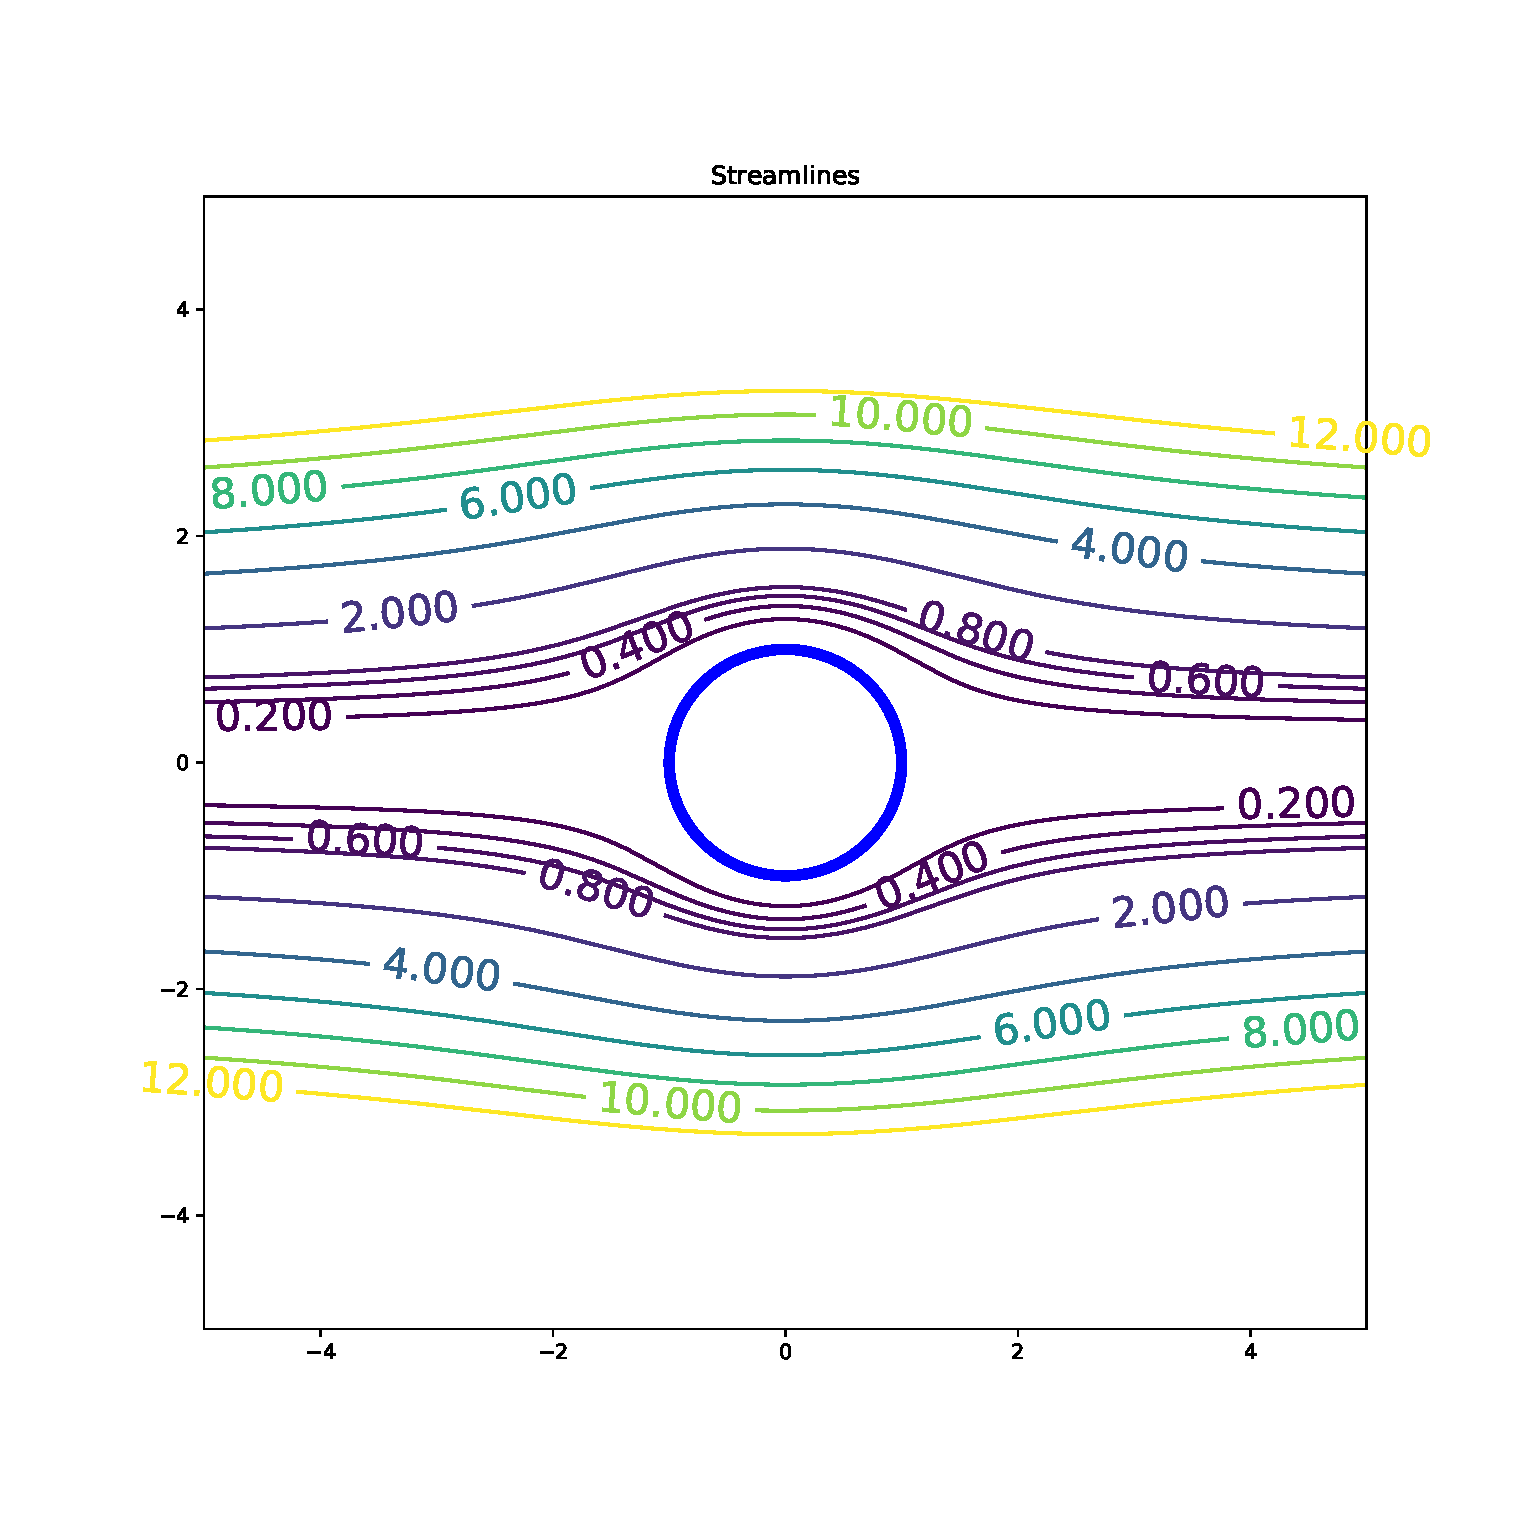
\includegraphics[width=0.8\linewidth]{figures/creeping_flow_past_sphere}

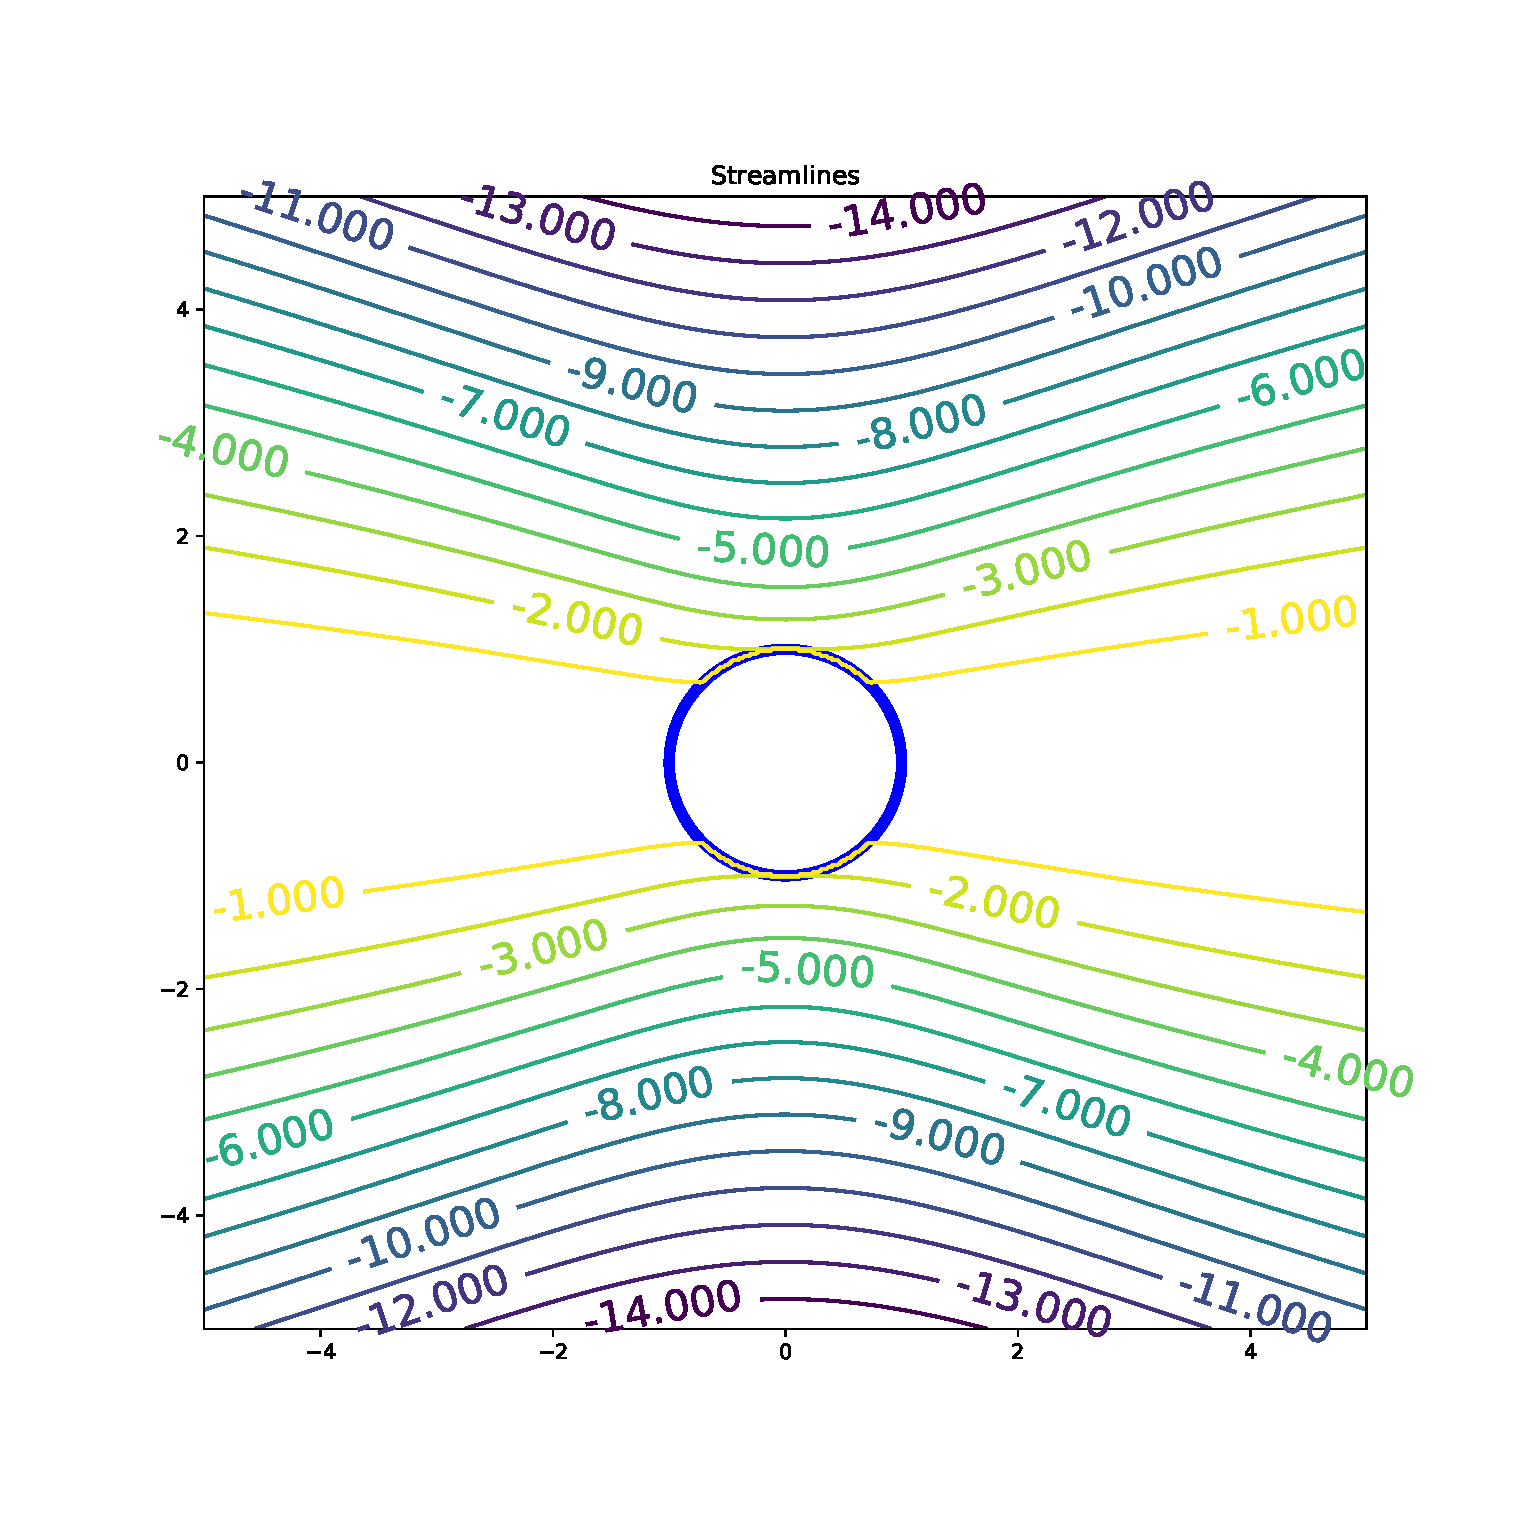
\includegraphics[width=0.8\linewidth]{figures/creeping_flow_past_sphere_moving}

\section{Around Stokes paradox*}
\label{sec:creeping_cylinder}

Stokes paradox is very soon encountered. Our task is to solve the
bi-Laplace equation, Eq. \ref{eq:bi-laplacian}, for a 2D case, in
which the vector potential $\bfA$ only has a $z$ component, equal
to the stream function $\psi$. Then,
\[
  \nabla^4 \psi = 0 ,
\]
from which $u=\nabla\times\psi$. Finally, the pressure field is
obtained from Stokes equation, \ref{eq:Stokes}:
$\nabla p = \mu \nabla^2 \bfu$.

In polar coordinates,
\begin{equation}
  \label{eq:Lapl_in_polar}
  \nabla^2 \psi =
  {1 \over  r}{\partial \over \partial  r}\left(
    r {\partial f \over \partial  r}\right)
  + {1 \over  r^2}{\partial^2 f \over \partial \theta^2} .
\end{equation}

Trying a function $\psi = r^\alpha \sin\theta$, we find that
\begin{equation*}
  \nabla^2   r^\alpha \sin\theta  =
  r^{\alpha-2} \sin\theta \left( \alpha^2 -1  \right) .
\end{equation*}

This means the only two possibilities are $\alpha=\pm 1$. Indeed, the
potential solution for the flow past a cylinder was built from these
two solutions (see e.g. Eq \ref{eq:pot_phi_guess}).

The bi-Laplacian is then
\begin{equation*}
  \nabla^4   r^\alpha \sin\theta  =
  r^{\alpha-4} \sin\theta
  \left( \alpha^2 -1  \right)
  \left( (\alpha-2)^2 -1  \right) .
\end{equation*}
The ``new'' possible exponents are now $\alpha=3$ and $\alpha=1$. The
first one is of no use, since it leads to the wrong behavior away from
the cylinder. The second one is not new at all! We are therefore stuck
with the same functional set as for potential flow.

This means that the only sensible solution is the potential one, which
of course features free-slip boundary conditions on the surface of the
cylinder. The resulting pressure field will be constant, since
$\nabla p = \mu \nabla^2 \bfu$, but these two functions have null
Laplacian. This field would, however, have a non-zero shear stress on
the cylinder, as we will discuss below.

The traditional way of dealing with this situation is to reject Stokes
equation \ref{eq:Stokes} as an adecuate model of the situation. The
perturbation in the velocity field is so great that any Reynolds
number is bound to be not so small after that --- in the sense that
the relevant length in Re=$\rho L u_0 /\mu$ is surely not the radius
of the cylinder, but a much larger value.

We present here an exploration of another way past this issue, which
could be interesting, but is -- we caution the reader -- fraught with
tricks.

Let us consider the next term, $\psi = r^\alpha \sin (2 \theta)$. Then
\begin{align*}
  \nabla^2   r^\alpha \sin(2 \theta)  &=
                                        r^{\alpha-2} \sin(2\theta) \left( \alpha^2 -4  \right) \\
  \nabla^4   r^\alpha \sin(2 \theta)  &=
                                        r^{\alpha-4} \sin(2\theta) \left( (\alpha-2)^2 -4  \right) .
\end{align*}
The solutions are then: $\alpha=\pm 2$ for the Laplace equation, and
$\alpha=0$ and $4$ for the bi-Laplacian. Again, the $2$ and $4$
exponents are to be rejected, but we may combine the $0$ and $-2$ ones
(remembering the latter is a solution of Laplace equation.)

Let us write
\[
  \psi =
  R u_0 \left[ \frac{r}{R} - \frac{1}{r} \right] \sin\theta -
  R w_0 \left[ 1 - \left( \frac{R}{r}\right)^2 \right] \sin( 2\theta) ,
\]
where $w_0$ is some unknown velocity.

The second term is chosen this way because the radial velocity
component is then
\begin{equation*}
  u_r= \frac{1}{r}\frac{\partial \psi}{\partial \theta} =
  u_0 \left[ 1  - \left( \frac{R}{r}\right)^2 \right] \cos\theta -
  2 w_0 \left[ \frac{R}{r} - \left( \frac{R}{r}\right)^3 \right] \cos( 2\theta) ,
\end{equation*}
which vanishes at the cylinder surface, $r=R$.

The tangential velocity is
\begin{equation*}
  u_\theta= - \frac{\partial \psi}{\partial r} =
  - u_0 \left[ 1  + \left( \frac{R}{r}\right)^2 \right] \sin\theta +
  2 w_0 \left( \frac{R}{r}\right)^3 \sin( 2\theta) .
\end{equation*}

At the surface, then
\begin{equation*}
  u_\theta(R) =
  - 2 u_0 \sin\theta + 2 w_0 \sin( 2\theta) .
\end{equation*}

The value of $w_0$ therefore determines at which points of the
cylinder is the velocity null (these are actually lines, in the $z$
direction). Common sense dictates these points occur at angles between
$0$ and $\pi/2$. This means $w_0$ should be positive, and comparable
to $u_0$. The simplest choice will be taken here, $w_0 = u_0$,
resulting in angles $\theta=\pm \pi/3$, at which the velocity is zero.
The resulting streamlines are plotted in
\ref{fig:creeping_flow_past_cyl}. The figure is very pleasing, which
is our original motivation in exploring this matter. The streamlines
as we move with the cylinder,
Fig. \ref{fig:creeping_flow_past_cyl_moving} are equally pleasing.

\begin{figure}
  \centering
  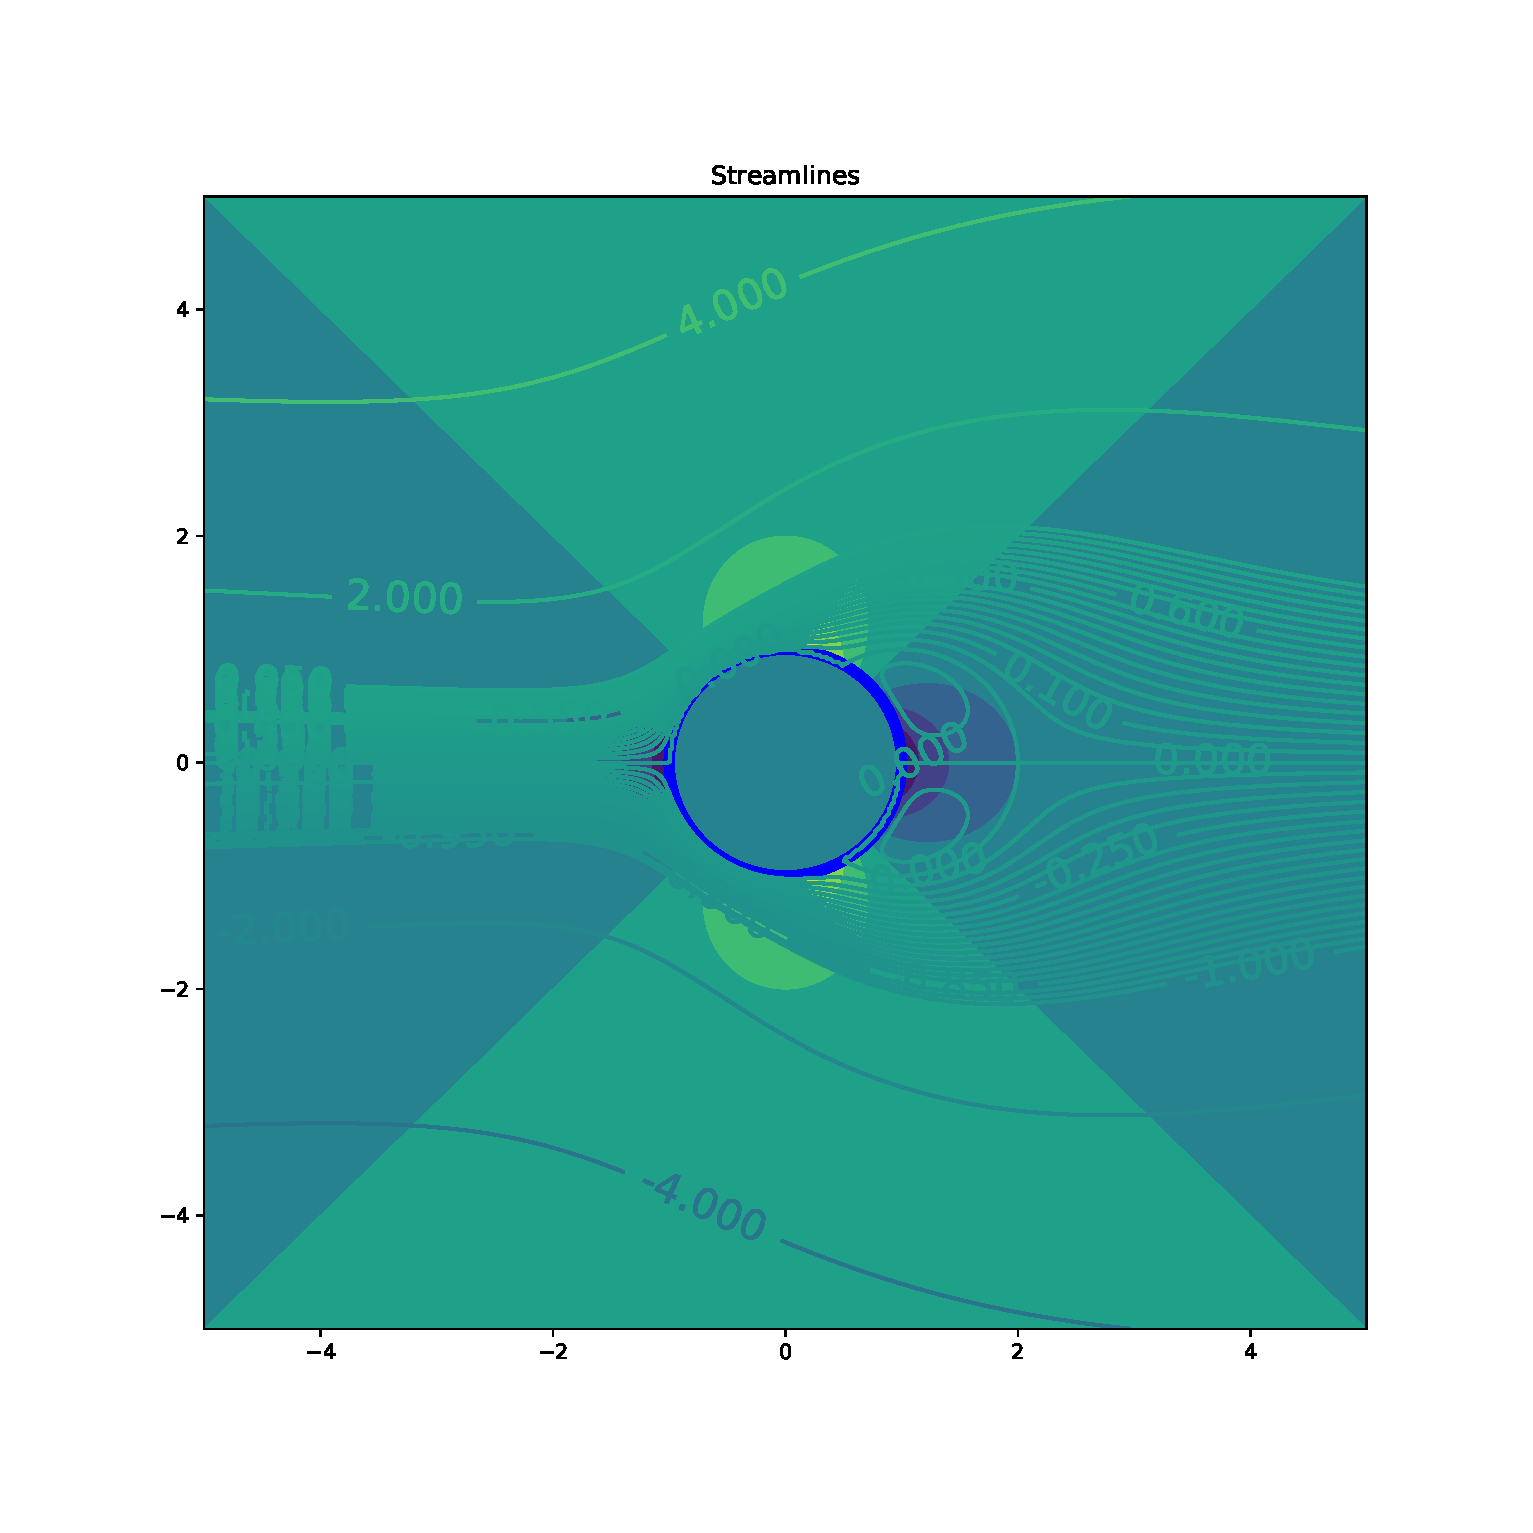
\includegraphics[width=0.8\linewidth]{figures/creeping_flow_past_cyl_slip}
  \caption{\label{fig:creeping_flow_past_cyl}}
\end{figure}


\begin{figure}
  \centering
  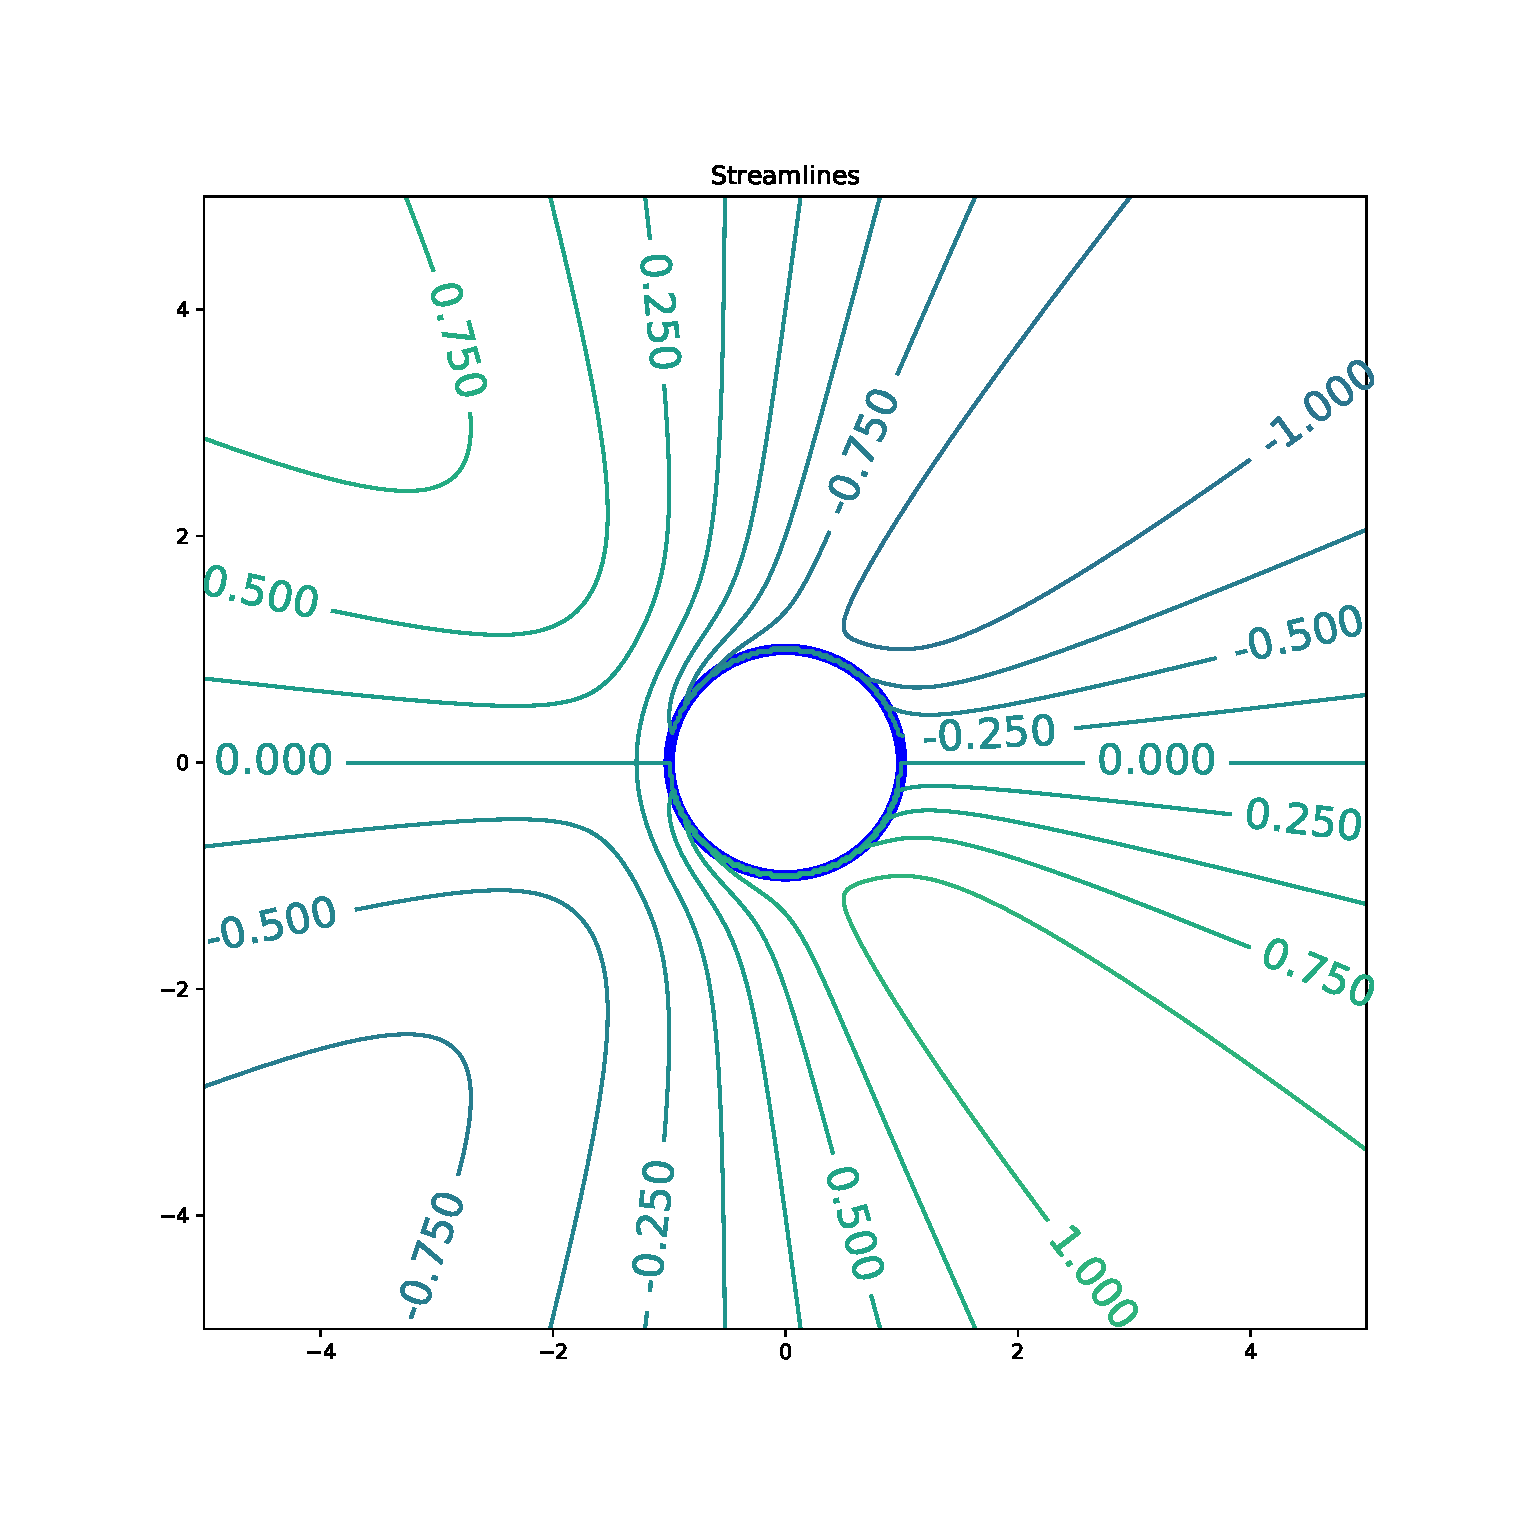
\includegraphics[width=0.8\linewidth]{figures/creeping_flow_past_cyl_slip_moving}
  \caption{\label{fig:creeping_flow_past_cyl_moving}}
\end{figure}


The resulting pressure field only has a non-trivial contribution from
the $\alpha=0$ term, since all other three are harmonic
(i.e. solutions of Laplace equation.)

The vector Laplacian is given by
\begin{align*}
(\nabla^2\bfu)_r &= \nabla^2 u_r - \frac{u_r}{r^2} - \frac{2}{r^2}
           \frac{\partial u_\theta}{\partial \theta} \\
(\nabla^2\bfu)_\theta &= \nabla^2 u_\theta - \frac{u_\theta}{r^2} + \frac{2}{r^2}
           \frac{\partial u_r}{\partial \theta} ,  
\end{align*}
with the scalar $\nabla^2$ expression as before in Eq.
\ref{eq:Lapl_in_polar}. We obtain
\begin{align*}
  (\nabla^2\bfu)_r &=   \frac{8 R u_0}{r^3} \cos(2 \theta)  \\
  (\nabla^2\bfu)_\theta &=    \frac{8 R u_0}{r^3} \sin(2 \theta)   .
\end{align*}

The pressure field is obtained from $\nabla p = \mu \nabla^2 \bfu$,
which in polar coordinates reads
\begin{align*}
  (\nabla p)_r     &=               \frac{\partial p }{  \partial r } = \mu(\nabla^2\bfu)_r  \\
  (\nabla p)_\theta &=  \frac{1}{r} \frac{\partial p }{  \partial \theta } = \mu(\nabla^2\bfu)_\theta ,
\end{align*}
whose solution is
\[
  p =
  -\frac{4 \mu u_0 R }{r^2} \cos(2\theta) =
  -\frac{4 \mu u_0}{R} \left( \frac{R }{r} \right)^2 \cos(2\theta) .
\]
In the last expression we make it clear that the pressure value is set
by $\mu u_0 / R$, and therefore the total pressure force upon the
cylinder is $D_p \sim p L R \sim \mu u_0 L$. The drag force would then
be independent of the radius, as predicted in
Eq. \ref{eq:drag_cyl_guess}. This is all consistent, if somewhat
surprising, but nevertheless moot: this pressure field, with its
$\cos(2\theta)$, has a d'Alembert's paradox! Indeed, by the same
arguments as in the classical potential solution, the net pressure
force is null. This is obvious in
Fig. \ref{fig:creeping_flow_past_cyl}, where the pressure field shows
a left-right symmetry.  Mathematically,
\begin{equation}
  \label{eq:pressure_drag_on_cyl_creeping}
  \frac{  D_p }{L} =
    R \int_0^{2\pi} d\theta   p \cos\theta  =
    4 \mu u_0 \int_0^{2\pi} d\theta  \cos\theta  \cos(2\theta)  = 0.
\end{equation}
Also, the sign of the pressure is troublesome: the low-pressure areas
are at the fore and aft of the cylinder, contrary to what may be
expected (and what is found for the potential solution,
Eq. \ref{eq:press_at_cyl_pot}.)

There is now another source of drag: shear stress on the surface. The
expression for the relevant part of the stress tensor is
\[
  \tau_{r\theta} = \mu \left(
    \frac1r
    \frac{\partial u_r}{\partial \theta} +
    r \frac{\partial }{\partial r} \left( \frac{u_\theta}{r}\right) 
  \right) 
\]
(i.e. it looks exactly as in spherical coordinates).

After some computations, at the surface we obtain
\[
  \tau_{r\theta} (R)  =  \frac{4 \mu u_0}{R} \left(
    \sin\theta - 2 \sin(2\theta) 
  \right) .
\]
The surprise is, then, that the term due to the potential solution,
$\sin\theta$, will result in a net drag force, but the new one will
not. Indeed, this force will be
\begin{equation}
  \label{eq:viscous_drag_on_cyl_creeping}
  \frac{  D_\tau }{L} =
   R \int_0^{2\pi} d\theta  (- \tau_{r\theta}) (- \sin\theta)  =
  4 \mu u_0 \int_0^{2\pi} d\theta  \sin^2\theta  =  4 \pi \mu u_0 .
\end{equation}
Notice there is a minus sign due to projection on the $x$ axis from
the tangential direction, and another due to the shear on the cylinder
being the reaction of the shear of the cylinder on the fluid.

The drag coefficient, defined as for the sphere (with an exposed area
now given by $2RL$), would be
\[
  C_\mathrm{inertial} = \frac{  2 D }{ \rho u_0^2 (2 R L) } =
  \frac{ 4 \pi \mu u_0   }{ \rho u_0^2  R L } =
  8\pi \frac{1}{\mathrm{Re}} ,
\]
with a Reynolds numberdefined in term of the diameter $2R$:
\[
  \mathrm{Re} = \frac{ \rho u_0 ( 2 R ) }{ \mu } .
\]

Notice that we have only employed two terms of what may be an
infinite expansion in terms $\sin(n\theta)$. In this way, by means of
Fourier analysis, we would be able to produce any tangencial velocity
we wished on the surface of the cylinder. The question is, of course,
which is the ``right'' distribution, since our main target, a null
velocity, is the one that is the one that is ruled out. For instance,
we could make the velocity null at the trailing edge of the cylinder
only.

Even if we did this, the potential would not be free of the
d'Alambert's paradox: all terms would ultimately be of the form
$\cos(n\theta)$, and the resulting drag would be zero for the same
reason as for $n=2$ in Eq. \ref{eq:pressure_drag_on_cyl_creeping}.

Moreover, the shear stress would also not change! Indeed, the new
terms in the stress tensor would be of the form $\sin(n\theta)$ ---
their contribution to the drag force would be null: in Eq.
\ref{eq:viscous_drag_on_cyl_creeping} it is clear that only $n=1$ may
contribute to this force. Since the only velocity contributing is the
potential solution, whose value is fixed by the up-stream velocity, it
cannot change.


\chapter{The viscous boundary layer}

\section{Stagnation flow}

In order to provide a glimse into the difficulties that are
encountered as soon as one ventures into slightly more complicated
problems, let us work out a solution of Navier-Stokes equations for a
simple stagnation situation.

The potential flow solution for a stady-state incompressible 2D
stagnation flow pattern close to a flat wall is given by the stream
function
\[
\psi = B x y ,
\]
from which,
\[
\begin{cases}
  & u_x =  \frac{\partial \psi}{\partial y} =   B x \\
  & u_y = -\frac{\partial \psi}{\partial x} = - B y .
\end{cases}
\]

The parameter $B$ has units of inverse time, and is given in practical
situations by $u_0 / L$, where $u_0$ is a relevant upstream velocity,
and $L$ a relevant size.

Recalling what we learned about potential flow and its relationship
with complex analysis, since $\psi = (B/2) \Im (z^2)$, it is easy to guess the
correct potential: $\phi=\Re( z^2) = (B/2) (x^2 + y^2)$.

This flow pattern looks roughly correct, see
Fig. \ref{fig:stagnation_streamlines} left, where the streamlines are
shown, along with the pressure. The latter follows from Bernoulli
principle:
\begin{equation}
  \label{eq:p_stag_pot}
p =
 -\frac{1}{2} \left[
  u_x ^2 +
  u_y^2
  \right] =
-\frac{1}{2} \left[
  (B x)^2 +
  (-B y)^2
  \right].  
\end{equation}


\begin{figure}
  \centering
  \includegraphics[width=0.4\linewidth]{figures/stagnation_potential_streamlines}
  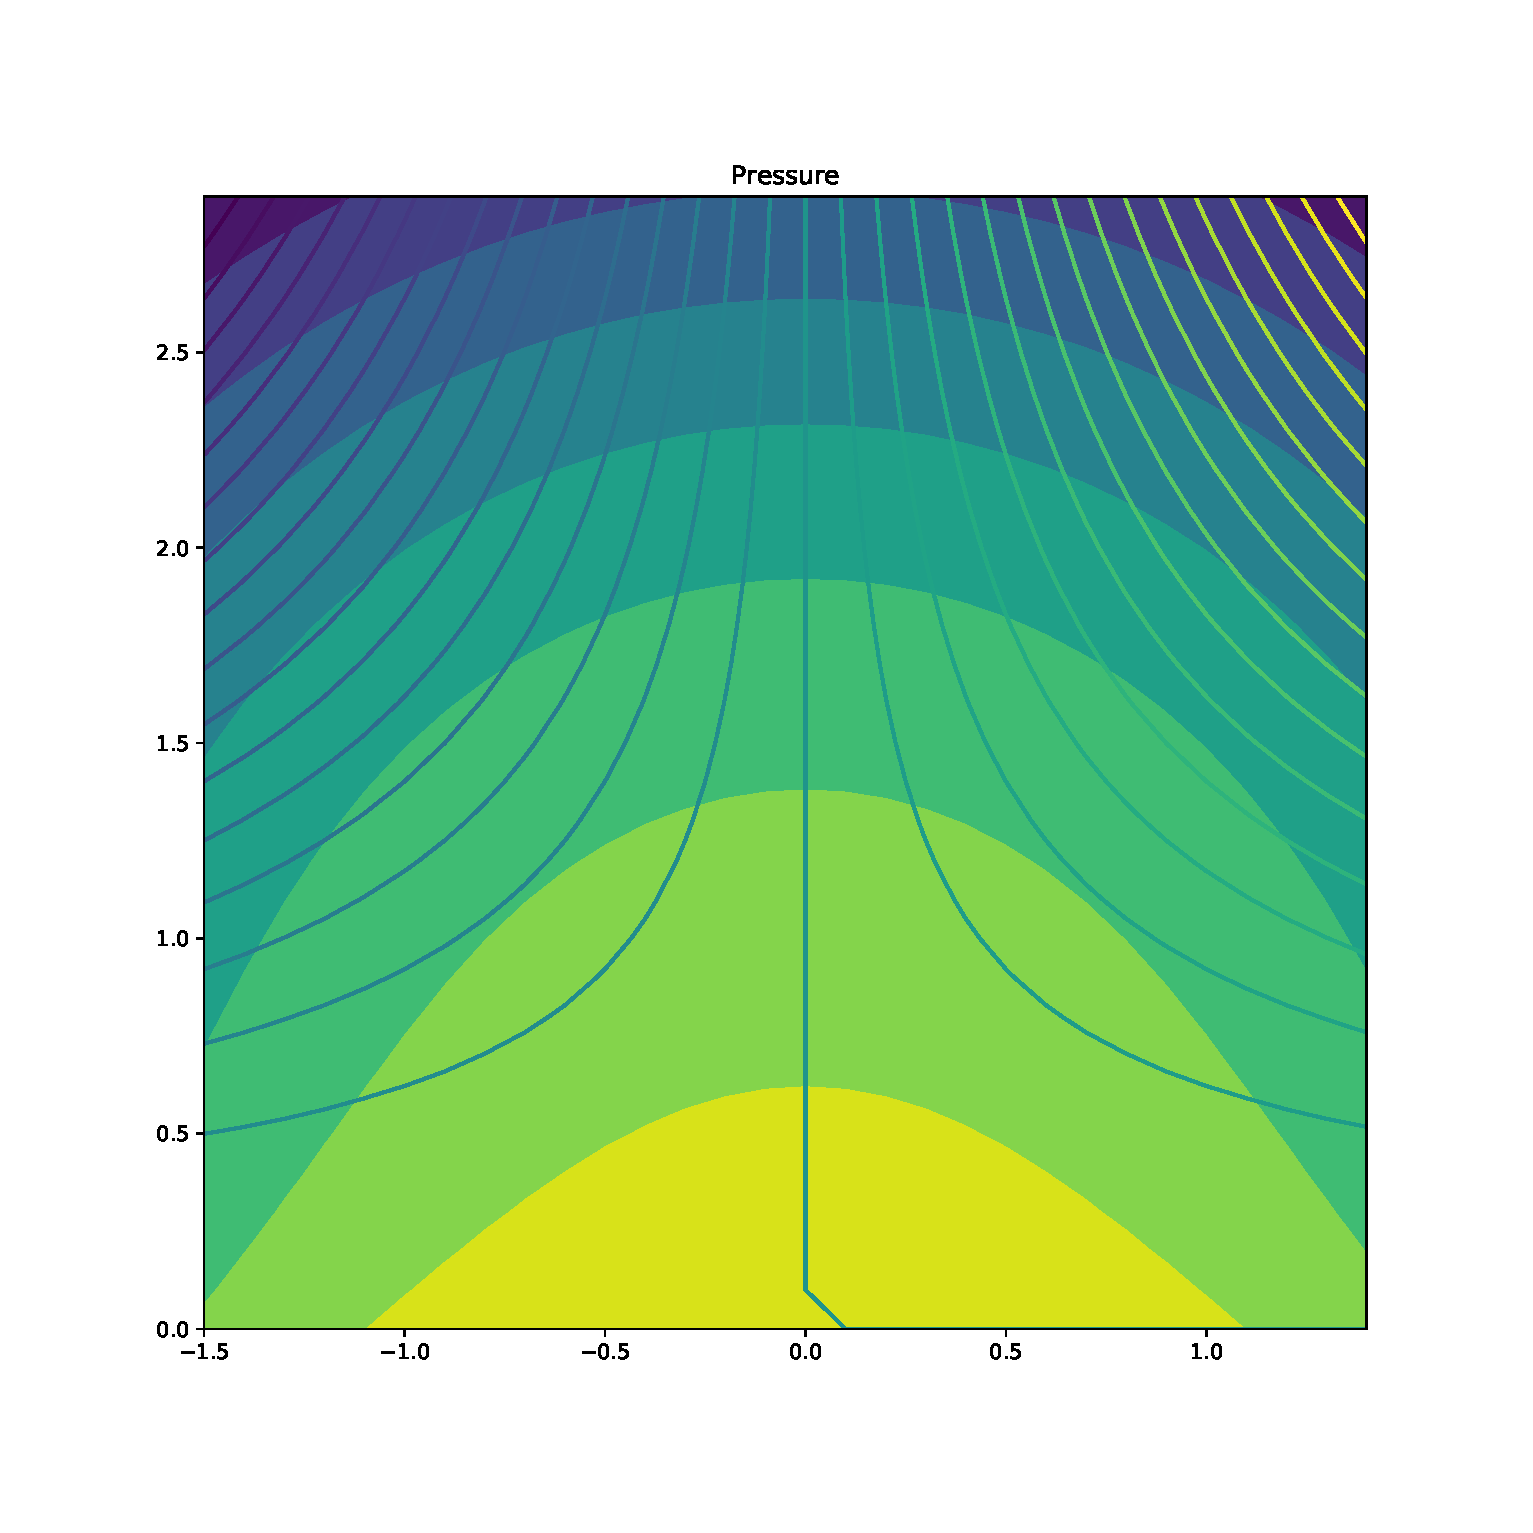
\includegraphics[width=0.4\linewidth]{figures/stagnation_viscous_streamlines}
  \caption{\label{fig:stagnation_streamlines}}
\end{figure}

But of course, at the wall ($y=0$) the fluid flows freely along the
wall. This means the boundary conditions are of the ``slip'' kind,
instead of the more realistic ``no-slip'' kind.

In order to find a correct flow, let us us the ansatz, originally
investigated by Hiemenz in 1911\footnote{%
  Hiemenz was a student of Prandtl, the founder of the theory of
  viscous boundary layers.
}.
  \[
\psi = B x f(y) ,
\]
where $f$ is a function of $y$ only. This is basically a separation of
variables, also guessing a linear dependence on $x$.

The velocity is now,
\[
\begin{cases}
  & u_x =   B x f' \\
  & u_y = - B f .
\end{cases}
\]
The correct no-slip condition then implies $f(0)=f'(0)=0$. We will
also require $f'(\infty)\to 1$ in order to recover our previous,
potential flow, solution.

Now, the steady 2D Navier-Stokes equations read
\begin{align}
  u_x  \frac{\partial u_x}{\partial x} +
  u_y  \frac{\partial u_x}{\partial y} 
  & =   - \frac{\partial p}{\partial x} +
  \nu
  \left(
  \frac{\partial^2 u_x}{\partial x^2} +
  \frac{\partial^2 u_x}{\partial y^2}
  \right) \\
  u_x  \frac{\partial u_y}{\partial x} +
  u_y  \frac{\partial u_y}{\partial y} 
  & =   - \frac{\partial p}{\partial y} +
  \nu
  \left(
  \frac{\partial^2 u_y}{\partial x^2} +
  \frac{\partial^2 u_y}{\partial y^2}
  \right) .
\end{align}
(Here, $p$ is not the true pressure, but the ``kinematic pressure'',
$p/\rho$. For convenience, a $\rho$ factor is assimilated into it, in
the same way that $\nu=\mu/\rho$.)

The $x$ equation is then reduced to
\[
 (B x f') (B f') + (-B f) B x f'' =  - \frac{\partial p}{\partial x} +
\nu B x f''' ,
\]
which may be written as
\[
B f f'' - B (f')^2 + \nu f''' = \frac{1}{B x} \frac{\partial
  p}{\partial x}  .
\]
Now, the left part of the equation is a function of $y$ only. This
means the pressure can only have this form:
\[
p(x,y) = C x^2 + h(y) ,
\]
with a constant $C$ and a function of $h$ to be determined later. Moreover,
as $y$ gets large we want to recover the potential solution. In this limit,
\[
f \to a + y \qquad f' \to 1 \qquad f'' \to 0 \qquad f'''\to 0 ,
\]
so the equation in this limit is
\[
- B \to  \frac{2 C x }{B x} ,
\]
which means $C =-B/2$, to be used later when solving for the pressure.

We must then solve
\[
 B \left(  f f'' + 1-  (f')^2 \right) + \nu f''' = 0 .
\]

Now, a lot may be learned from the shape of an equation without even
solving it. Let us look for a similarity transformation of the
form
\[
f(y) = b g(a y) ,
\]
so that equation for $f$ may be cast as an equation for $g$ with no
parameters. With this prescription,
\[
f' = ba g' \qquad f''=b a^2 g'' \qquad f'''= b a^3 g''' ,
\]
So then the equation reads
\[
 B \left(  b^2 a^2 g g'' + 1-  b^2 a^2 (g')^2 \right) + \nu b a^3  g''' = 0 .
\]
Because of the ``$1$'' in the parenthesis, it is clear $b=1/a$, so then,
\[
 B \left(  g g'' + 1-  (g')^2 \right) + \nu  a^2  g''' = 0 .
\]
Therefore, if $a=\sqrt{B/\nu}$,
\begin{equation}
  \label{eq:Z_ode}
  g g'' + 1-  (g')^2  +  g''' = 0 ,
\end{equation}
with no parameters, as we wanted. This means that, whichever solution
we find, our $f$ is going to be given by
\[
f(y) = \sqrt{\frac{\nu}{B}} g\left(\sqrt{\frac{B}{\nu}}  y  \right) =
\sqrt{\frac{\nu}{B}} g\left(\frac{y}{ \sqrt{\nu/B} } \right) =
 \ell g\left(\frac{y}{ \ell } \right) .
\]
Clearly, $\ell = \sqrt{\nu/B} $ sets the scale of variation of the
flow away from its potential solution.

Notice that the velocities will be
\[
\begin{cases}
  & u_x =   B x g'(y/\ell) = B\ell \frac{x}{\ell} g'(y/\ell)  \\
  & u_y = - B \ell g(y/\ell)  ,
\end{cases}
\]
so that the velocity scale is set by $B\ell=\sqrt{B\nu}$.


%The $y$ equation reduces, with our velocities, to
%\[
%B^2 f f' = - \frac{\partial p}{\partial y} - B\nu f'' .
%\]
%This means that $\frac{\partial p}{\partial y}$ is a function of $y$
%only.



Our task is then to integrate the non-linear ODE \ref{eq:Z_ode}, subject
to these boundary conditions:
\[
g(0)=0 \qquad g'(0)=0 \qquad g''(x\to \infty) \to 0 .
\]
If we had a condition on $g''(0)$, the problem would be a
straight-forward exercise in integration. However, we have instead a
condition on the other side of the integration domain, which makes
this problem somewhat harder. The technique should then be a
``shooting method'', in which $g''(0)$ is adjusted until a vanishing
small of $g''$ far away is found. The procedure may be made
systematic, but we can also fiddle a bit with the parameters in order
to find a reasoable approach. It is quite easy to arrive at
$g''(0)\approx 1.234$, as in the jupyter python notebook at
Supplementary Material.

%How far is far away may be again estimated from the equation.


\begin{figure}
  \centering
  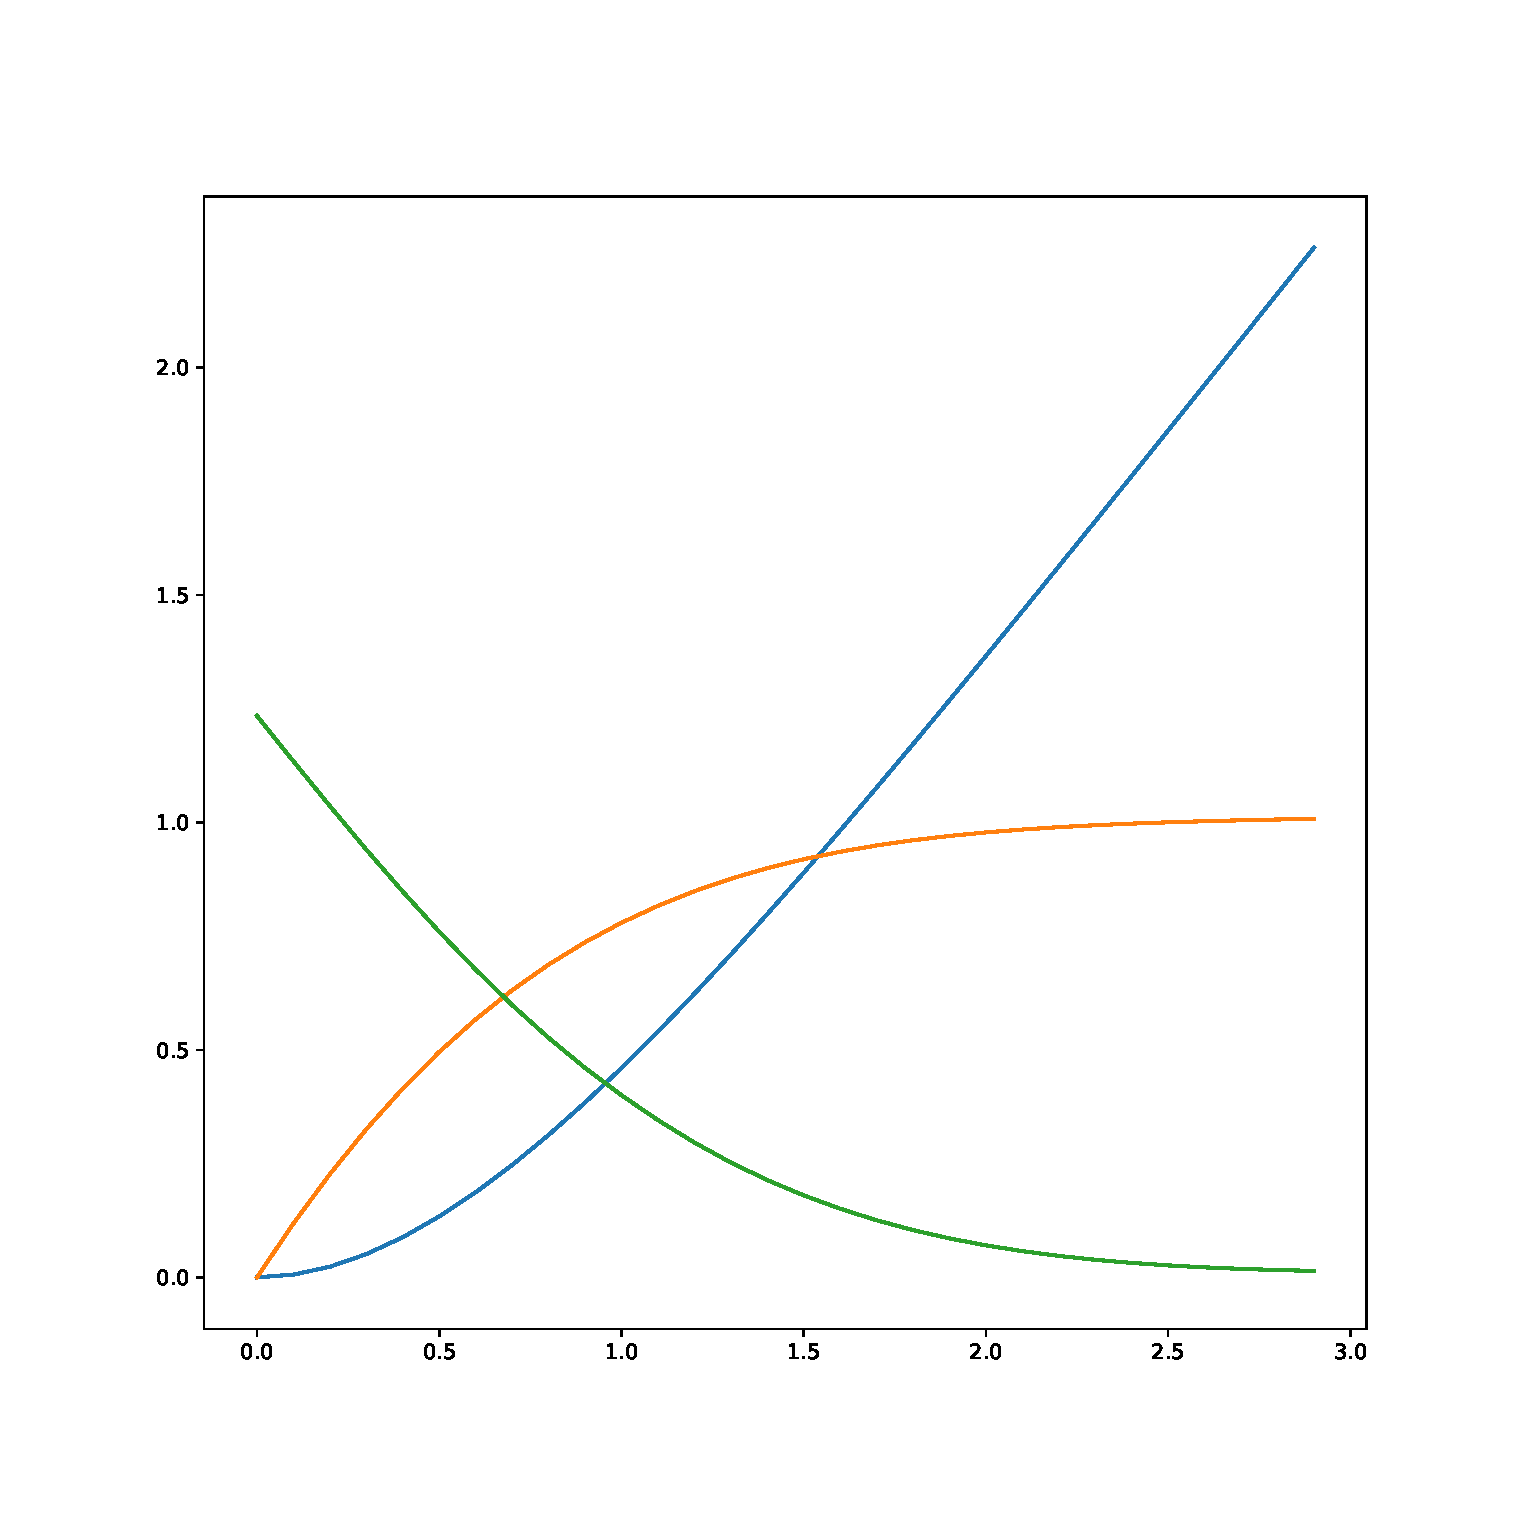
\includegraphics[width=0.4\linewidth]{figures/stagnation_functions}
    \includegraphics[width=0.4\linewidth]{figures/stagnation_function_disp}
  \caption{\label{fig:stagnation_functions}}
\end{figure}


In Figure \ref{fig:stagnation_functions} left, the function $g$ and
its first and second derivatives are plotted. With these, it is easy
to plot the resulting streamlines, Figure
\ref{fig:stagnation_streamlines} right. In the latter, the potential
streamlines are shown in the left. It is apparent how the flow is
``moved upwards'' due to viscous effects near the wall. This
displacement is readily quanfified by the asympotic behavour of $g$,
as shown in Figure \ref{fig:stagnation_functions} left. A reasonable
approximation is
\[
g(y) \approx -0.64 + y .
\]
This provides an estimate of the boundary layer thickness as given
by
\[
\delta = 0.64 \ell =  0.64 \sqrt{\nu/B} ,
\]
which then increases as the root square of $\nu$, and decreases as,
basically, the root square of the velocity far away from the wall
(through $B$).

To get some numbers, if air approaches a \SI{10}{\centi\meter} diameter
cylinder at $u_0=\SI{10}{\meter\per\second}$, then
$B = 4u_0/D =\SI{400}{\per\second}$ (there is a factor of $4$
involved, see \cite{white} \S 7.3 ). With
$\nu\approx\SI{1.5e-5}{\meter\squared\per\second}$, we get
$\delta = \SI{0.12}{\milli\meter}$, a very thin layer. The thickness of
the layer can be defined in other ways, for example as the distance at
which $f'(y) \approx 0.99 $ (so that the value of $u_x = B x f'$ is
$99\%$ its potential solution value, $B x$.) This yields
$\approx 2.4 \ell$, which is about $3.7$ times larger than
$\delta$. Still, only approximately $ \SI{0.44}{\milli\meter}$, beyond
which the effect of the wall is quite neglibible.

This fact is a blessing, since it restores our faith in
potential-based solutions: many flows look potential flows when viewed
at some distance from obstacles (indeed, away from any region that may
generate vorticity and involve shear, such as jets, wakes \ldots). It
also solves d'Alembert's paradox, since the velocity field can still
comply with the no-slip boundary condition and exert drag forces on
obstacles (in general, they will be due both to pressure and to wall
shear stress). It is also a curse mathematically: the details of a
proper matching between it the layer and the flow around it must be
worked out carefully. Also computationally, the fact that the boundary
layer is so thin compared with other dimensions of the problem leads
to prohibitively large simulation meshes, or the necessity to refine
the meshes close to surfaces. The latter fact favours methods such as
the finite element method, or the finite volume method, in which
refinement is easier, over other ones like finite differences.

The pressure was partly known already, $p=-(B^2/2) x^2 + h(y)$. The other
Navier-Stokes equation, which we have still not used, reads
\[
B f B f'  =  - \frac{\partial p}{\partial y} -
\nu B  f'' .
\]
This means
\[
h' = - B^2 f f' - \nu B f'' ,
\]
which may be easily integrated :
\[
h = -B^2 \frac12 f^2  - \nu B f' .
\]
So, finally:
\[
p = -\frac{1}{2} \left[
  (B x)^2 +
  (B f)^2
  \right]  - \nu B f' =
 -\frac{1}{2} \left[
  (u_x / f' )^2 +
  u_y^2
  \right]  - \nu B f' ,
 \]
 where in the last equality it is shown how the pressure is not so
 different from the potential solution, Eq. \ref{eq:}.
%
 Notice it is not $u_X$ which features, but rather $u_x/f'$, which
 does tend to the $u_x$ away from the wall. An additional, viscous
 term appears, which makes the pressure have a constant offset
 $-\nu B$ with respect to its potential counterpart, as we move
 away from the wall.

 Pressures are also included in Fig.
 \ref{fig:stagnation_streamlines}. To make a more quantitative
 comparison, isobars are plotted in
 Fig. \ref{fig:stagnation_pressures}. It is interesting that viscosity
 causes pressure to be ``pushed'' against the wall, flattening the
 isobars (and, interestingly, making them not normal to the
 wall). While, far away from the wall, they approach the same circular
 shape, but with a constant offset. In these figures, pressures are
 plotted in their reduced form. It is easy to check that the pressure
 scale is given by $B \nu$ (units of velocity squared --- remember this
 is the dynamic pressure).

\begin{figure}
  \centering
  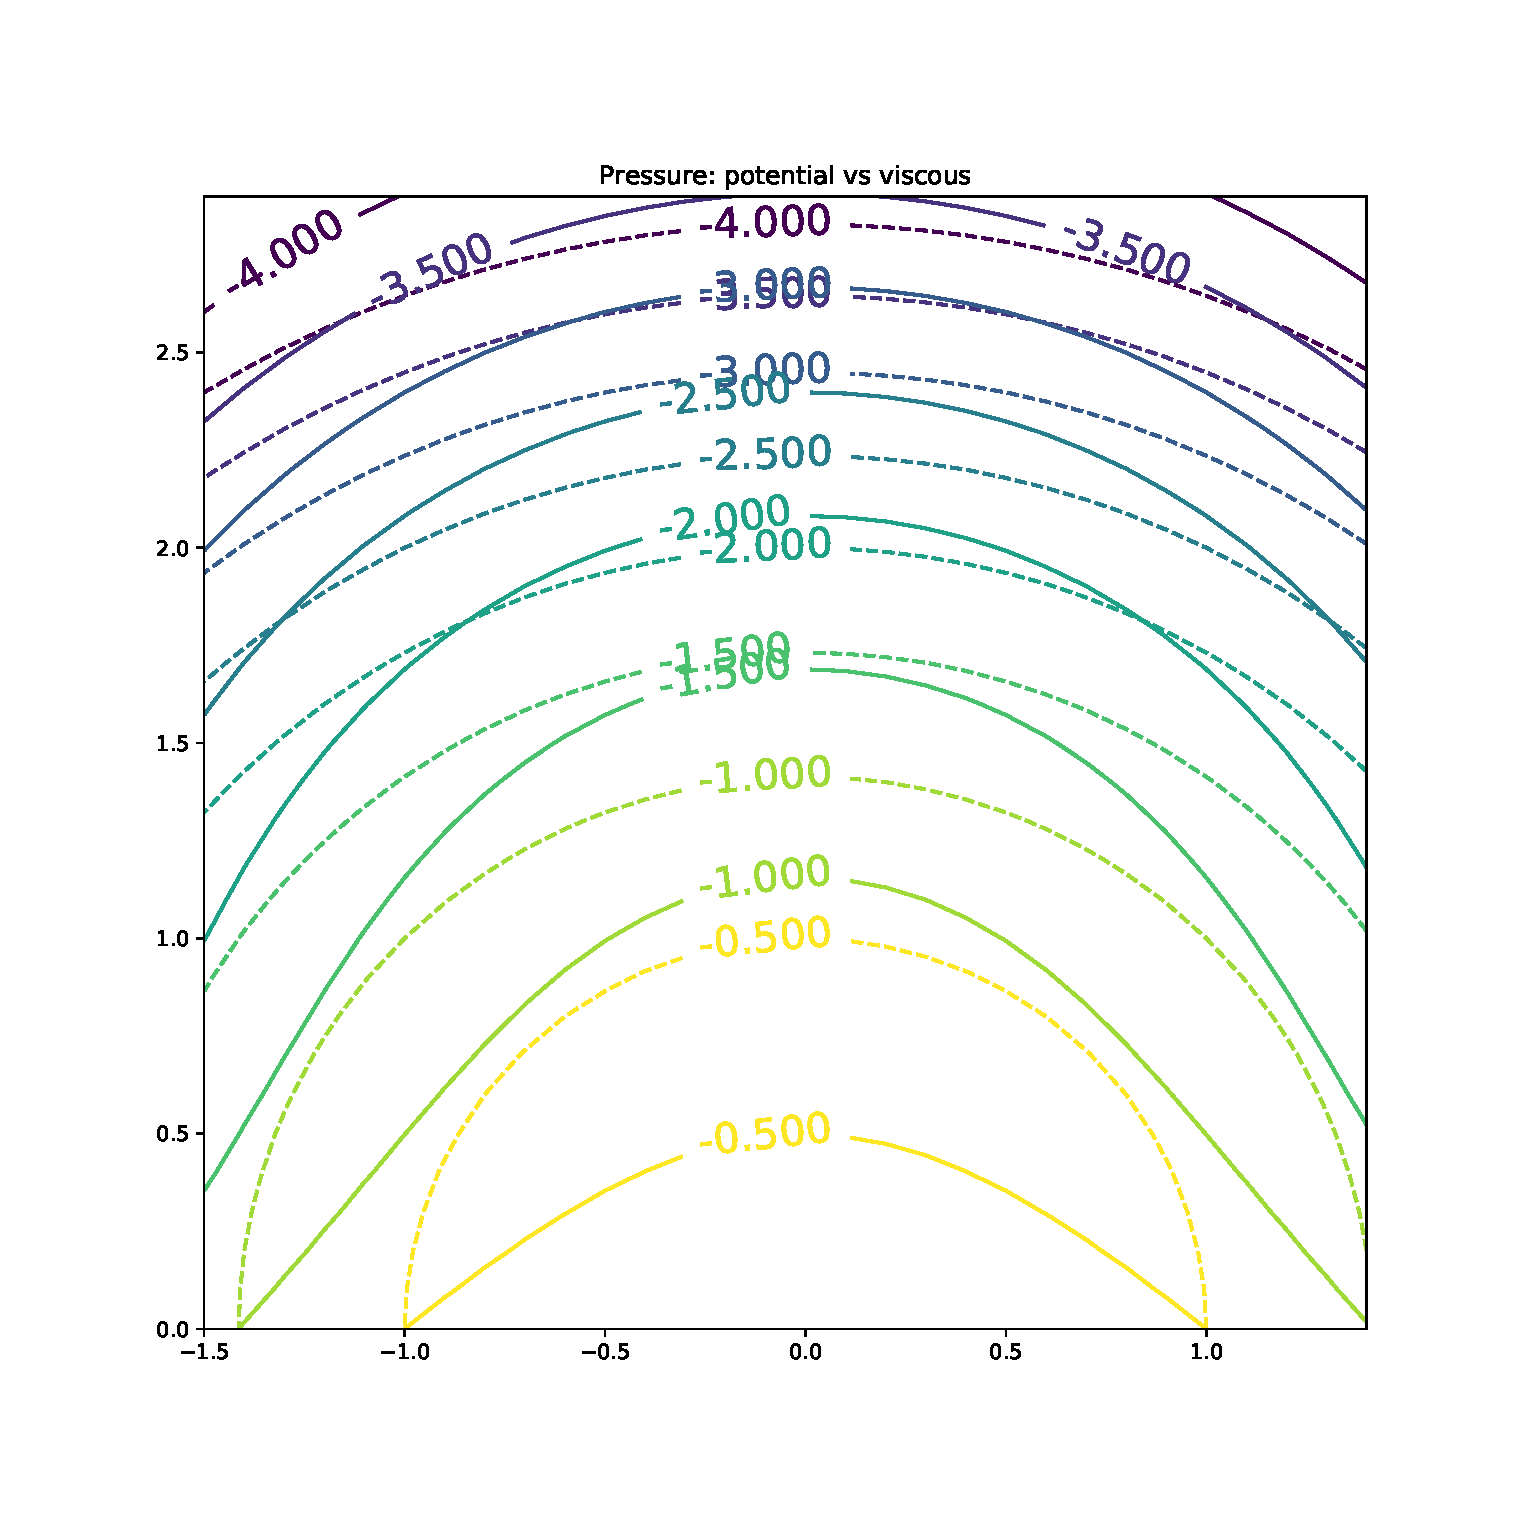
\includegraphics[width=0.6\linewidth]{figures/stagnation_potential_viscous_pressures}
  \caption{\label{fig:stagnation_pressures}}
\end{figure}

Another interesting feature of the flow is its vorticity, which is
readily computed from
\[
\omega_z =
\frac{\partial u_y}{\partial x} -
\frac{\partial u_x}{\partial y} =
0 - B x f''(y)  = - B x^* g''(y^*) .
\]
Hence the wall is seen to induce vorticity close to it, with a sign change
on both sides on the $x=0$ symmetry plane. The shear stress is given by a
similar expression,
\[
\tau_{xy}= \mu
\left(
\frac{\partial u_y}{\partial x} +
\frac{\partial u_x}{\partial y}
\right)
 =  \mu B  x f''(y)  = \mu B x^* g''(y^*) .
 \]

 In particular, the wall stress is
 \[
 \tau_\mathrm{w}:=\tau_{xy}(y=0) = \mu B x^* g''(0)
 \approx 1.234 \mu B x^*
 \]

 The (horizontal) skin friction coefficient may be defined, for this problem,
 as
 \[
 C_\mathrm{f} := \frac{2 \tau_\mathrm{w} }{ \rho (B x)^2 } .
 \]
 The denominator features the horizontal velocity away from the wall,
 $B x$. Then,
 \[
 C_\mathrm{f} := \frac{2 \sqrt{B\nu}  g''(0) }{ B x } =:
 \frac{2   g''(0) }{\sqrt{ \mathrm{Re}_x} } ,
 \]
 where the local Reynolds number is defined as
 \[
 \mathrm{Re}_x = \frac{(Bx) x}{\nu} .
 \]
 I.e. a Reynolds number where the typical velocity is the horizontal
 velocity far from the wall, $Bx$, and the distance is that to the
 impact point, $x$. A dependence of the friction coefficient with the
 inverse square root of a local Reynolds number is a common feature of
 laminar boundary layers.
 


%\chapter{Turbulence}

%% to be merged onto creeping.tex

If we try $\psi=r^2 \sin^2\theta$ we find
\[
  {\cal L} \psi = \left[ a(a-1) - 2 \right] r^{a-2} \sin^2\theta ,
\]
so the possible exponent values for ${\cal L} \psi = 0$ are $a=2$ and
$a=-1$ (this basically solves the potential flow problem.)

Notice that, once again, the outcome contains a function that is very
similar to the input. This means that, applying twice the differential
operator we will get
\[
  {\cal L}^2 \psi =
  \left[   a  (a-1) - 2 \right]
  \left[ (a-2)(a-3) - 2 \right]
  r^{a-4} \sin^2\theta ,
\]
so  the possible exponent values for ${\cal L}^2 \psi = 0$ are $a=2$ and
$a=-1$, as before, plus $a=4$ and $a=1$.

The solution we try will be a combination of all four posibilities --- but
the $a=4$ we can discard right away because it is too high a divergence. Let
us write
\[
  \psi = u_0 \left[ \frac12 r^2 + \frac{A}{r} + B r \right] \sin^2\theta .
\]
Then our boundary conditions at $r=R$ imply
\begin{align*}
  \left.\frac{\partial \psi}{\partial r}\right|_{r=R} = 0 &\implies
                                                            R-\frac{A}{R^2} + B  =0 \\
  \left.\frac{\partial \psi}{\partial \theta}\right|_{r=R} = 0 &\implies
                                                            \frac12 R^2-\frac{A}{R} + BR  =0 ,
\end{align*}
from which we may obtain $A$ and $B$, and finally write the solution
\[
  \psi = \frac12 u_0 R^2
  \left[\left(  \frac{r}{R} \right)^2
    + \frac12 \frac{R}{r} - \frac32 \frac{r}{R} \right] \sin^2\theta .
\]
The components of the velocity are readily found from
\ref{eq:u_from_psi_spherical},
\begin{equation*}
  \begin{split}
    u_r     &=  u_0  \left[
      1+ \frac12 \left(\frac{R}{r}\right)^3 - \frac32 \frac{R}{r}
    \right] \cos \theta \\
    u_\theta &=
    - u_0  \left[
      1
      - \frac14 \left(\frac{R}{r}\right)^3 - \frac34 \frac{R}{r}
    \right] \sin \theta
  \end{split}
\end{equation*}

The pressure is found from \ref{eq:}, and found to have a simple expression,
\[
  p=p_0 - \frac32 \frac{\mu u_0}{R} \left(\frac{R}{r}\right)^2
  \cos\theta ,
\]
where $p_0$ is the pressure far from the sphere. Notice this pressure
is harmonic, as discussed above. At the sphere surface,
\[
  p(r=R) = p_0 - \frac32 \frac{\mu u_0}{R} \cos\theta,
\]
with a high-pressure zone at the fore of the sphere (the point facing
the upstream direction, $\theta=\pi$), and a lower pressure at the aft
($\theta=0$). This clearly asymmetric pressure distribution results in
a net drag on the sphere
\[
  D_p=  - \int_S  p \cos\theta dA =
  -2\pi R^2 \int_0^\pi d\theta \sin\theta  p(\theta) \cos\theta =
  + 3 \pi \mu u_0 R \int_0^\pi d\theta \sin\theta  \cos^2\theta .
\]
The minus sign comes from the fact that we want the pressure upon the
sphere, which by reaction is opposite the pressure upon the fluid.
The last integral is immediate: the primitive is $-(1/3)\cos^3\theta$,
so the definite integral provides a $2/3$ factor. Finally,
\[
  D_p=  2 \pi \mu u_0 R .
\]
This agrees with our guess of \ref{eq:drag_sphere_guess}.

However, this drag force is due to pressure only. There will be an
additiona shear drag, which may be calculated from the shear stress.
The relevant component of the tensor is (see \cite{white1991viscous},
Eq. B17, p. 584):
\[
  \tau_{r\theta} = \mu \left(
    \frac1r
    \frac{\partial u_r}{\partial \theta} +
    r \frac{\partial }{\partial r} \left( \frac{u_\theta}{r}\right) 
  \right) .
\]

This can be computed to obtain
\[
  \tau_{r\theta} = 
  - \frac32 \frac{\mu u_0}{r} \left(\frac{R}{r}\right)^3 \sin\theta ,
\]
hence at the sphere surface,
\[
  \tau_{r\theta} (r=R) =  - \frac32 \frac{\mu u_0}{R}  \sin\theta .
\]
This looks very similar to the pressure, with a $\sin$ instead of a
$\cos$, which means the stress is maximal at the equator, which seems
reasonable. However, the contribution to the drag force is higher ---
twice higher, to be precise. Indeed,
\[
  D_\tau =  - \int_S  \tau_{r\theta} \sin\theta dA ,
\]
with a minus sign for the same reason as the pressure, and a $\sin$
because this is a shear stress, resulting in a force that is
tangential to the surface of the sphere.  Then
\[
  D_\tau =
  - 2\pi R^2 \int_0^\pi d\theta   \tau_{r\theta} \sin^2\theta  =
  3 \pi \mu u_0 R  \int_0^\pi d\theta \sin^3\theta .
\]
The primitive of $\sin^3\theta$ is, through
$\cos^2\theta=1-\sin^2\theta$, equal to
$(1/3) \cos^3\theta - \cos\theta$. The definite integral is then $4/3$, and
\[
  D_\tau = 4 \pi \mu u_0 R .
\]

The final drag force is the celebrated Stokes drag law: \index{Stokes drag law}
\[
  D_\tau = 6 \pi \mu u_0 R ,
\]
where $1/3$ of the drag is due to pressure and $2/3$ to shear stress.

Despite the shear having a contribution that is twice that two
pressure, notice that by writing 
\begin{align*}
  - p(r=R) + p_0 &= \bar{p} \cos\theta,  
  -\tau_{r\theta} (r=R) &= \bar{p} \sin\theta,  
\end{align*}
where $\bar{p} := - (3/2) \frac{\mu u_0}{R}$, it is apparent that the
normal force, due to pressure, and the tangential one, due to shear
stress, result from a decomposition of a force upon the sphere surface:
\[
  \bff := \frac32 \frac{\mu u_0}{R} \bhe_z .
\]
It is remarkable that this force is equal for every point on the
sphere.




FOR POTENTIAL.TEX:




In axisymmetric flow,
\[
  \divu =
  {1 \over r^2}{\partial \left( r^2 u_r \right) \over  \partial r} +
  {1 \over r\sin\theta}{\partial \over \partial  \theta} \left( u_\theta\sin\theta \right) ,
\]
but an equivalent expression is
\[
  \divu =
  {\partial \left( r^2 u_r \sin\theta \right) \over  \partial r} +
  {\partial \left( r u_\theta\sin\theta \right)  \over \partial  \theta}
\]

so continuity is trivially satisfied with the choice
\ref{eq:u_from_psi_spherical}.


From the curl in spherical coordinates,
\begin{align}
  u_r     &= \frac {1}{r\sin \theta }
            \frac{ \left( \partial A  \sin \theta \right) }{\partial \theta }  \\
  u_\theta &= -\frac1{r} \frac{\partial (rA) }{\partial r} 
\end{align}
and we find
\begin{equation}
%  \label{eq:u_from_psi_spherical}
  \begin{split}
    u_r     &=  \frac1{r^2 \sin\theta} \frac{\partial \psi}{\partial \theta} \\
    u_\theta &= -\frac1{r   \sin\theta} \frac{\partial \psi}{\partial r}
  \end{split}
\end{equation}



Notice $A=\psi / \rho $ also in spherical coordinates !

% \input{etc}

\nocite{*}

\bibliographystyle{plainnat}

\bibliography{fluid_mechanics}

\printindex

\begin{appendix}
   \listoffigures
   \listoftables
\end{appendix}




\end{document}
